%\RequirePackage{lineno}

\documentclass[aps,prc,preprint,superscriptaddress,showpacs,showkeys,amsmath]{revtex4-1}
%\documentclass[article,showpacs,preprintnumbers,amsmath,amssymb]{revtex4}
\usepackage{graphicx}
\usepackage[usenames,dvipsnames,svgnames,table]{xcolor}
\usepackage{rotating}
\usepackage{graphicx}% Include  files
\usepackage{dcolumn}% Align table columns on decimal point
\usepackage{bm}% bold math
\usepackage{epsfig}
\usepackage{hyperref}
\usepackage{ulem}
\usepackage{appendix}
\begin{document}

\newcommand{\Jpsi}{J/\psi}
\newcommand{\pT}{p_{T}}
\newcommand{\calO}{{\cal{O}}}
\newcommand{\barQ}{{\bar{Q}}}
\newcommand{\barq}{{\bar{q}}}
\newcommand{\barc}{{\bar{c}}}
\newcommand{\barb}{{\bar{b}}}
\newcommand{\baru}{\bar{u}}
\newcommand{\barv}{\bar{v}}
\newcommand{\barup}{\bar{u}_{+}}
\newcommand{\barum}{\bar{u}_{-}}
\newcommand{\barvp}{\bar{v}_{+}}
\newcommand{\barvm}{\bar{v}_{-}}
\newcommand{\charm}{{\rm{charm}}}
\newcommand{\bottom}{{\rm{bottom}}}

\newcommand{\cs}{{\hat{s}}}
\newcommand{\ct}{{\hat{t}}}
\newcommand{\cu}{{\hat{u}}}
\newcommand{\alphas}{{\alpha_{s}}}

%\newcommand{}{{}}

\newcommand{\shat}{\hat{\rm s}}
\newcommand{\that}{\hat{\rm t}}
\newcommand{\uhat}{\hat{\rm u}}
\newcommand{\zhat}{\hat{\rm z}}

\newcommand{\CA}{{\cal A}}
\newcommand{\Qbar}{{\overline Q}}
\newcommand{\QQbaroctetgen}{{Q\Qbar[ ^{2S+1}L_J^{(8)}]}}
\newcommand{\QQbaroctetsingS}{{Q\Qbar[ ^1S_0^{(8)}]}}
\newcommand{\QQbaroctettripP}{{Q\Qbar[ ^3P_J^{(8)}]}}
\newcommand{\QQbaroctettripPone}{{Q\Qbar[ ^3P_1^{(8)}]}}

\def\QQbaroctettripS{Q\Qbar[ ^3S_1^{(8)}]}
\def\QQbaroctetPzero{Q\Qbar[ ^3P_0^{(8)}]}
\def\QQbaroctetPone{Q\Qbar[ ^3P_1^{(8)}]}
\def\QQbaroctetPtwo{Q\Qbar[ ^3P_2^{(8)}]}

%\newcommand{\hatt}{\hat{t}}
%\newcommand{\hatu}{\hat{u}}
%\newcommand{\hats}{\hat{s}}


%\linenumbers
\title{{\Large Charmonia production in p+p collisions under NRQCD formalism}} 
\author{\large Vineet Kumar}
\affiliation{Nuclear Physics Division, Bhabha Atomic Research Center, Mumbai, India}
\author{\large Prashant Shukla}
\email{pshukla@barc.gov.in}
\affiliation{Nuclear Physics Division, Bhabha Atomic Research Center, Mumbai, India}
\affiliation{Homi Bhabha National Institute, Anushakti Nagar, Mumbai, India}
%\author{\large Ramona Vogt}
%\affiliation{Nuclear and Chemical Sciences Division, Lawrence Livermore National Laboratory, Livermore, CA 94551, USA}
%\affiliation{Physics Department, University of California, Davis, CA 95616, USA}
\date{\today}

\begin{abstract}

  This work presents the differential charmonia production cross sections in high 
energy p+p collisions calculated  using NRQCD formalism. The NRQCD formalism, 
factorizes the quarkonia production cross sections in terms of short distance QCD 
cross sections and long distance matrix elements (LDMEs). The short distance cross
sections are calculated in terms of perturbative QCD and LDMEs are obtained by 
fitting the experimental data. Measured transverse momentum distributions of 
$\chi_{\rm c}$, $\psi$(2S) and J/$\psi$ in p +{$\bar {\rm p}$} collisions at $\sqrt{s}=$ 1.8, 1.96 TeV 
and in p+p collisions at $\sqrt{s}=$  7, 8 and 13 TeV are used to constrain LDMEs. The feed-down 
contribution to each state from the higher states are taken into account.
  The formalism provides a very good description of the data in a wide energy range. 
The values of LDMEs are used to predict the charmonia cross sections in p+p collisions 
at 13 TeV in kinematic bins relevant for the LHC detectors. Charmonia ratios are
predicted at 1.8, 5 and 13 TeV  p+p collisions.

\end{abstract}

\pacs{12.38.Bx, 13.60.Le, 13.85.Ni, 14.40.Gx}
\keywords{quarkonia, NRQCD}

\maketitle

%%%%%%%%%%%%%%%%%%%%%%%%%%%%%%%%%%%%%%%%%%%%%%%%%%%%%%%%%%%%%%%%%%%%%%%%%%%%%%%%%

\section{Introduction}

 The quarkonia ($Q\bar Q$) have provided useful tools for probing both 
perturbative and nonperturbative aspects of Quantum Chromodynamics (QCD) 
eversince the discovery of J/$\psi$ resonance~\cite{Augustin:1974xw,Aubert:1974js}. 
 The Quarkonia states are qualitatively different from most other hadrons since 
the velocity $v$ of the heavy constituents is small allowing a 
non-relativistic treatment of bound states. 
  The quarkonia are the richest probes to study the bulk strongly interacting matter
produced in heavy ion collisions \cite{Kumar:2014kfa}. The ratios of excited to ground state 
quarkonia yields are considered as robust signals of Quark Gluon Plasma (QGP) and
measuring such ratios has become the most important goals of Pb+Pb experiments
at LHC \cite{Chatrchyan:2012lxa,Khachatryan:2014bva}.
%The quarkonia production process can be divided into two major parts
%\begin{enumerate}
%\item Production of a heavy quark pair in hard partonic collisions.
%\item Formation of quarkonia from the two heavy quarks.
%\end{enumerate}
  The heavy quarks due to their high mass 
($m_{\rm c}\,\sim$ 1.6 GeV/c$^2$, $m_{\rm b}\,\sim$ 4.5 GeV/c$^2$), 
are produced in initial partonic collisions with sufficiently high momentum 
transfers. Thus the heavy quark production can be treated 
perturbatively~\cite{Nason:1987xz,Nason:1989zy}.
  The formation of quarkonia out of the two heavy quarks is a nonperturbative 
process and is treated in terms of different 
models \cite{Bodwin:1994jh,Brambilla:2004wf}. 
  Most notable models for quarkonia production are the color-singlet
model (CSM), the color-evaporation model (CEM), the non-relativistic QCD
(NRQCD) factorization approach, and the fragmentation-function approach.

  In the CSM \cite{Einhorn:1975ua,Ellis:1976fj,Carlson:1976cd,Berger:1980ni},
it is assumed that the $Q\bar Q$ pair that evolves into
the quarkonium is in a color-singlet state and has the same spin
and angular-momentum as the quarkonium. 
 The production rate of quarkonium state is related to 
the absolute values of the color-singlet $Q\bar Q$ wave function and 
its derivatives, evaluated at zero $Q\bar Q$ separation. These quantities 
can be extracted by comparing calculated quarkonium decay
rates in the CSM with the experimental measurements. 
 The CSM was successful in predicting quarkonium production rates at
relatively low energy \cite{Schuler:1994hy} but, at high
energies, very large corrections appear at next-to-leading
order (NLO) and next-to-next-to-leading order (NNLO) in $\alpha_s$
\cite{Artoisenet:2007xi,Campbell:2007ws,Artoisenet:2008fc}.
  The NRQCD factorization approach comprise the color-singlet model, 
but also includes color-octet states.
    In the CEM~\cite{Fritzsch:1977ay,Amundson:1995em,Amundson:1996qr}, it
is assumed that the produced $Q\bar Q$ pair evolves into a quarkonium
if its invariant mass is less than the threshold for producing a 
pair of open-flavor heavy mesons. 
 The nonperturbative probability for the $Q\bar Q$ pair to evolve into 
a quarkonium state is fixed by comparison with the measured production
cross section of that quarkonium state.
 The CEM calculations provide good descriptions of the CDF data for J/$\psi$,
$\psi$(2S), and $\chi_{\rm c}$ production at $\sqrt{s}=1.8$~TeV
\cite{Amundson:1996qr} but it fails to predict the quarkonium 
polarization.

%In the fragmentation-function approach the inclusive
%quarkonium production cross sections is written  
%in terms of convolutions of parton production cross sections 
%with light-cone fragmentation functions~\cite{Nayak:2005rw,Nayak:2005rt}.
%This procedure provides a convenient way to organize the contributions
%to the cross section in terms of powers of $m_Q/p$.
%The contribution to the cross section at the
%leading power in $m_Q/p_T$ is given by the production of a single parton
%({\it e.g.}, a gluon), at a distance scale of order $1/p_T$, which
%subsequently fragments into a heavy quarkonium
%\cite{Braaten:1996pv}.  The contribution to the cross section at the
%first sub-leading power in $m_Q/p_T$ is given by the production of a
%$Q\bar Q$ pair in a vector- or axial-vector state, at a distance scale of
%order $1/p_T$, which then fragments into a heavy quarkonium.

  In the NRQCD factorization approach \cite{Bodwin:1994jh},
the probability for a $Q\bar Q$ pair to evolve into a quarkonium is expressed
as matrix elements of NRQCD operators in terms of the heavy-quark velocity 
$v$ in the limit $v\,\ll\,1$. This approach takes into account the complete structure of 
the $Q\bar Q$ Fock space, which is spanned by the state $n\,=\,^{2S+1}L_{J}^{[a]}$ 
with spin $S$, orbital angular momentum $L$, total angular momentum $J$, 
and color multiplicity $a$ = 1 (color-singlet), 8 (color-octet). 
 The $Q\bar Q$ pairs which are produced at short distances in color-octet (CO) states, 
evolve into physical, color-singlet (CS) quarkonia by emitting soft gluons 
nonperturbatively.
 In the limit $v\rightarrow0$, the CSM is recovered in the case of S-wave quarkonia.
 The short distance cross sections can be calculated within the 
framework of perturbative QCD (pQCD). The long distance matrix elements (LDME) 
corresponding to the probability of the $Q\barQ$ state to convert to the quarkonium 
can be estimated by comparison with the experimental measurements. 
  The leading order (LO) NRQCD gives a good description of J/$\psi$ yields at 
RHIC, Tevatron and LHC energies~\cite{Sharma:2012dy}.

  The NLO corrections to color-singlet J/$\psi$ production have been investigated 
in Refs.~\cite{Campbell:2007ws,Gong:2008sn}. The color-singlet J/$\psi$ 
production is found to be enhanced by 2-3 order of magnitude in high 
$p_T$ region~\cite{Gong:2008sn}.
% and its polarization changes from transverse into longitudinal at NLO~\cite{Gong:2008sn}. 
 The NLO corrections to J/$\psi$ production via S-wave 
color octet (CO) states ($^1S_{0}^{[8]}\,^3S_{1}^{[8]}$) are studied in 
Ref.~\cite{Gong:2008ft} and the corrections to $p_{T}$ distributions of both 
J/$\psi$ yield and polarization are found to be small. In Refs.~\cite{Ma:2010vd}, 
NLO corrections for $\chi_{cJ}$ hadroproduction are also studied. 

  Several NLO calculations are performed to obtain the polarization and yield of
J/$\psi$. The J/$\psi$ polarization presents a rather confusing 
pattern~\cite{Butenschoen:2012px,Chao:2012iv,Gong:2012ug}.
  The works of Ref.~\cite{Butenschoen:2010rq} and  Ref.~\cite{Ma:2010jj} present
NLO-NRQCD calculations of J/$\psi$ yields.
  In both the works, the set of CO LDMEs fitted to $p_{T}$ distributions measured 
at HERA and CDF are used to describe the $p_{T}$ distributions from RHIC and 
the LHC.
 The fitted LDMEs of Ref.~\cite{Butenschoen:2010rq} and  Ref.~\cite{Ma:2010jj}
are incompatible with each other. A recent work~\cite{Shao:2014yta} gives 
calculations for both the yields and polarizations of charmonia at the Tevatron 
and the LHC where the LDMEs are obtained by fitting the Tevatron data only.
  With the LHC running for several years we now have very high quality quarkonia 
production data in several kinematic regions up to very high transverse momentum 
which could be used to constrain the LDMEs. In this paper, we use CDF data
\cite{Abe:1997yz,Abe:1997jz,Acosta:2004yw,Abulencia:2007bra} along with new LHC data 
\cite{Chatrchyan:2011kc,Khachatryan:2015rra,Chatrchyan:2012ub,Aad:2015duc,ATLAS:2014ala},
\cite{Aaij:2012ag,Aaij:2011jh,Aaij:2015rla,Aaij:2013dja} to constrain 
the LDMEs. 
 The feed-down contribution to each state from the higher states are taken into account.
These new LDMEs are then used to predict the J/$\psi$ and $\psi$(2S)
cross-section at 13 TeV for the kinematical bins relevant to LHC detectors.
 The NLO calculations are still evolving and thus we use LO calculations in 
this work. The values of fitted LDMEs with LO formulations are always useful 
for straightforward predictions of quarkonia cross section and for the 
purpose of a comparison with those obtained using NLO formulations.
 The uncertainties in the LDMEs due to NLO are quantified. We also give predictions
for the $\psi$(2S) to J/$\psi$ ratios at $\sqrt{s}=$ 5 TeV which has 
become important due to the recent Pb+Pb collisions at $\sqrt{s_{NN}}=$ 5 TeV. 



%%%%%%%%%%%%%%%%%%%%%%%%%%%%%%%%%%%%%%%%%%%%%%%%%%%%%%%%%%%%%%%%%%%%%%%%%%%%%%%%%%%%%%%
\section{Quarkonia Production in p$+$p collisions}
\label{section:ppProduction}
 The NRQCD formalism provides a theoretical framework for studying the heavy 
quarkonium production. The dominant processes in the production of heavy 
mesons $\psi$ are $g+q\rightarrow \psi+q$, $q+\bar{q}\rightarrow \psi+g$ and 
$g+g\rightarrow \psi+g$. We represent these processes by $a+b\rightarrow \psi+X$, 
where $a$ and $b$ are the light incident partons. The invariant cross-section 
for the production of $\psi$ can be written in a factorized form as 
\begin{equation}
  %\begin{split}
    E\frac{d^{3}\sigma^{\psi}}{d^{3}p} = \sum_{a,b}\int \int dx_a\,dx_b \, 
    G_{a/p}(x_a,\mu_{F}^{2}) \, G_{b/p}(x_b,\mu_{F}^{2}) \, \frac{\hat s}{\pi}\frac{d\sigma}{d\hat t}
    \otimes \delta(\hat s + \hat t + \hat u -M^{2}), 
%\end{split}
\label{eqn:cross}
\end{equation}
where $G_{a/p}(G_{b/p})$ is the distribution function (PDF) of the incoming parton 
$a(b)$ in the incident proton, which depends on the momentum fraction $x_a(x_b)$, 
the factorization scale $\mu_F$ and on the renormalization scale $\mu_R$. 
We take $\mu_F$ = $\mu_R$.
 The parton level  Mandelstam variables ${\hat s}$, ${\hat t}$, and ${\hat u}$
can be expressed in terms of $x_a$, $x_b$ as 
\begin{equation}
\begin{split}
\cs = \,& x_{a}\,x_{b}\,s \\
\ct = \,& M^{2} - x_{a}\,\sqrt{s}\,m_{T}\,e^{-y}\\
\cu = \,& M^{2} - x_{b}\,\sqrt{s}\,m_{T}\,e^{y} ,
\end{split}  
\end{equation}
 where $\sqrt{s}$ being the total energy in the centre-of-mass, $y$ is the rapidity 
and $p_{T}$ is the transverse momentum of the $Q\bar Q$ pair. Writing 
down $ \hat s + \hat t + \hat u -M^{2} = 0$ and solving for $x_{b}$ we obtain
\begin{equation}
x_b = \frac{1}{\sqrt{s}}\frac{x_a\,\sqrt{s}\,m_T\,e^{-y}-m^2_H}{x_a\,\sqrt{s}-m_T\,e^y}.
\end{equation}
 The double differential cross-section upon $p_{T}$ and $y$ then is obtained as
\begin{equation}
\frac{{d^{2}\sigma}^{\psi}}{dp_T\,dy} = \sum_{a,b}\int_{x_{a}^{min}}^{1} dx_a\, 
           G_{a/A}(x_a,\,\mu^{2}_{F})\, G_{b/B}(x_b,\,\mu^{2}_{F})\times 
            2p_T \frac{x_a\,x_b}{x_a-\frac{m_T}{\sqrt{s}}e^y}\frac{d\sigma}{d\hat t},
\end{equation}
where the minimum value of $x_a$ is given by
\begin{equation}
x_{a\rm min} = \frac{1}{\sqrt{s}}\frac{\sqrt{s}\,m_T\,e^{y}-m^2_H}{\sqrt{s}-m_T\,e^{-y}}.
\end{equation}












 The parton level cross-section $d\sigma/d\hat{t}$ is defined as~\cite{Bodwin:1994jh}
\begin{equation}
\frac{d\sigma}{d\hat t} = \frac{d\sigma}{d\hat t}(ab\rightarrow Q\overline{Q}(^{2S+1}L_{J})+X)
               \, M_{L}(Q\overline{Q}(^{2S+1}L_{J})\rightarrow\psi).
\end{equation}
  The short distance contribution 
$d\sigma/d\hat t (ab\rightarrow Q\overline{Q}(^{2S+1}L_{J})+X)$ 
corresponds to the production of a $Q\barQ$ pair in a particular
color and spin configuration can be calculated within the framework of 
perturbative QCD (pQCD). The long distance matrix elements (LDME) 
$M_{L}(Q\overline{Q}(^{2S+1}L_{J})\rightarrow\psi)$ corresponds to the 
probability of the $Q\barQ$ state to convert to the quarkonium wavefunction
and can be estimated by comparison with experimental measurements. 
 The short distance invariant differential cross-section is given by
\begin{equation}
  \frac{d\sigma}{d\hat t}(ab\rightarrow Q\overline{Q}(^{2S+1}L_{J})+X) 
                = \frac{|\mathcal{M}|^2}{16\pi{\hat s}^2},
\end{equation}
where $|\mathcal{M}|^2$ is the Feynman squared amplitude. We use the expressions for the 
short distance CS cross-sections given in 
Refs.~\cite{Baier:1983va,Humpert:1986cy,Gastmans:1987be} and the CO 
cross-sections given in Refs.~\cite{Cho:1995vh,Cho:1995ce,Braaten:2000cm} which
we reproduce in the Appendix A. 
  The CTEQ6M~\cite{Lai:2010vv} parametrization is used for parton 
distribution functions. 




   The LDMEs scale with a definite power of the relative velocity $v$ of the 
heavy quarks inside $Q\bar Q$ bound states. In the limit $v<<1$, the production of 
quarkonium is based on the $^3S_1^{[1]}$ and $^3P_J^{[1]}$ ($J$ = 0,1,2) CS states 
and $^1S_0^{[8]}$, $^3S_1^{[8]}$ and $^3P_J^{[8]}$ CO states. The differential 
cross section for the direct production of $J/\psi$ can be written as the 
sum of these contributions,
\begin{equation}
\begin{split}
d\sigma(J/\psi) &= d\sigma(Q\barQ([^3S_1]_{1}))
                   \,M_{L}(Q\barQ([^3S_1]_{1})\rightarrow J/\psi) 
                +  d\sigma(Q\barQ([^1S_0]_{8}))
                   \,M_{L}(Q\barQ([^1S_0]_{8})\rightarrow J/\psi)\\ 
                &+  d\sigma(Q\barQ([^3S_1]_{8}))
                   \,M_{L}(Q\barQ([^3S_1]_{8})\rightarrow J/\psi) 
                +  d\sigma(Q\barQ([^3P_0]_{8}))
                   \,M_{L}(Q\barQ([^3P_0]_{8})\rightarrow J/\psi)\\ 
                &+  d\sigma(Q\barQ([^3P_1]_{8}))
                   \,M_{L}(Q\barQ([^3P_1]_{8})\rightarrow J/\psi)
                +  d\sigma(Q\barQ([^3P_2]_{8}))
                   \,M_{L}(Q\barQ([^3P_2]_{8})\rightarrow J/\psi)\\
                &+ \cdot\cdot\cdot  
\label{eq:dsigmaJ}
\end{split}
\end{equation}
  The dots represent contribution of terms at higher powers of $v$. The 
contributions from the CO matrix elements in Eq.~\ref{eq:dsigmaJ} are suppressed 
by $v^4$ compared to the CS matrix elements.


  For the case of the $p$-wave bound states $\chi_{cJ}$ ($\chi_{c0}$, $\chi_{c1}$ 
and $\chi_{c2}$), the color-singlet state $Q\barQ[^3P_J]_{1}$ and the color-octet 
state $Q\barQ[^3S_1]_{8}$ contribute to the same order in $v$ ($v^{5}$) because of 
the angular momentum barrier for the $p-$wave states, and hence both need to be included. 
The $\chi_{c}$ differential cross section thus can be written as 
\begin{equation}
\begin{split}
d\sigma(\chi_{cJ}) =\,&d\sigma(Q\barQ([^3P_J]_{1}))
                   \,M_{L}(Q\barQ([^3P_J]_{1})\rightarrow \chi_{cJ}) 
                +  d\sigma(Q\barQ([^3S_1]_{8}))
                   \,M_{L}(Q\barQ([^3S_1]_{8})\rightarrow \chi_{cJ})\\
                &+ \cdot\cdot\cdot  
\label{eq:dsigmachi}
\end{split}
\end{equation}
%Similar expressions hold for the $\chi_b(1P)$, $\chi_b(2P)$ and $\chi_b(3P)$ mesons.  
  The prompt $J/\psi$ production at LHC energies consists of direct $J/\psi$ 
production from the initial parton-parton hard scattering and the feed-down contributions 
to the $J/\psi$ from the decay of heavier charmonium states $\psi(2S)$, 
$\chi_{c0}$, $\chi_{c1}$ and $\chi_{c2}$.  The relevant branching fractions are given 
in the Table~\ref{table:CharmoniaBFs} \cite{Nakamura:2010zzi}. 
The prompt $\psi(2S)$ has no significant feed-down contributions from the higher mass states. 

\begin{table*}[h]
\caption{Relevant branching fractions for charmonia~\cite{Nakamura:2010zzi}}.
\begin{tabular}{c|cccc}
Meson From &to $\chi_{c0}$ &to $\chi_{c1}$ &to $\chi_{c2}$ &to $J/\psi$\\ 
\hline
$\psi(2S)$ & 0.0962 & 0.092 & 0.0874 & 0.595   \\
$\chi_{c0}$& &  &  & 0.0116           \\
$\chi_{c1}$& &  &  & 0.344           \\
$\chi_{c2}$& &  &  & 0.195           \\
\hline
\end{tabular}
\label{table:CharmoniaBFs}
\end{table*}

  The expressions and the values for the color-singlet operators can be found 
in~\cite{Cho:1995ce,Cho:1995vh,Eichten:1994gt} which are obtained by solving the 
non-relativistic wavefunctions.
 The CO operators can not be related to the non-relativistic
wavefunctions of $Q\barQ$ since it involves a higher Fock state and thus
measured data is used to constrain them.
  The color-singlet contributions along with their calculated values 
and color-octet contributions to be fitted are written below for the prompt
$J/\psi$.

%\begin{equation}
%\begin{split}
% &M_{L}(c\barc([^3S_1]_{1})\rightarrow J/\psi) = 3 \,M_{L}(c\barc([^1S_0]_{1})\rightarrow J/\ps%i) 
%           = 3N_c\frac{|R_{n=1}(0)|^2}{2\pi} = 1.2\;{\rm GeV^3} \;, \\
% &M_{L}(c\barc([^3S_1]_{1})\rightarrow \psi(2S))=3 \,M_{L}(c\barc([^1S_0]_{1})\rightarrow \psi(2S)) 
%                = 3N_c\frac{|R_{n=2}(0)|^2}{2\pi}=0.76\;{\rm GeV^3} \;, \\
% &\frac{1}{5} M_{L}(c\barc([^3P_2]_{1})\rightarrow \chi_{c2}(1P)) 
%        = \frac{1}{3} \,M_{L}(c\barc([^3P_1]_{1})\rightarrow \chi_{c1}(1P)) 
%         =\,M_{L}(c\barc([^3P_0]_{1})\rightarrow \chi_{c0}(1P)) \\
% & = 3N_c\frac{|R^\prime_{n=1}(0)|^2}{2\pi} =0.054 \, m_{\charm}^2\;{\rm GeV^3}. 
%\label{eq:charmsinglet}
%\end{split}
%\end{equation}
%  Here $R(0)$ is the radial wavefunction and $R^\prime(0)$ is its first derivative 
%at the origin, and $n$ refers to the radial quantum 
%number. 
% We use measured data from LHC~\cite{Chatrchyan:2011kc,Khachatryan:2015rra,Aad:2015duc} 
%and TeVatron~\cite{Acosta:2004yw} to constrain these  CO Matrix elements.
% Yields of $\psi(2S)$ have been measured at TeVatron~\cite{Abe:1997yz} and 
%LHC~\cite{Chatrchyan:2011kc}. Data for $\chi_{cJ}$ are available from 
%TeVatron~\cite{Abe:1997yz}.  






\begin{enumerate}
\item{Direct contributions
\begin{equation}
\begin{split}
&M_{L}(c\barc([^3S_1]_{1})\rightarrow J/\psi) = 1.2\,{\rm GeV}^{3}\\
&M_{L}(c\barc([^3S_1]_{8})\rightarrow J/\psi) \\
&M_{L}(c\barc([^1S_0]_{8})\rightarrow J/\psi) \\
&M_{L}(c\barc([^3P_0]_{8})\rightarrow J/\psi) = M_{L}(c\barc([^3S_1]_{8})\rightarrow J/\psi) \, m_c^2
~\label{eq:Mpsi1}
\end{split}
\end{equation}
    }
\item{Feed-down contribution from $\psi(2S)$
\begin{equation}
\begin{split}
&M_{L}(c\barc([^3S_1]_{1})\rightarrow \psi(2S)) = 0.76\,{\rm GeV}^{3}\\
&M_{L}(c\barc([^3S_1]_{8})\rightarrow \psi(2S)) \\
&M_{L}(c\barc([^1S_0]_{8})\rightarrow \psi(2S)) \\
&M_{L}(c\barc([^3P_0]_{8})\rightarrow \psi(2S)) = M_{L}(c\barc([^3S_1]_{8})\rightarrow \psi(2S))\, m_c^2 
~\label{eq:Mpsi2}
\end{split}
\end{equation}
  }
\item{Feed-down contribution from $\chi_{cJ}$
\begin{equation}
\begin{split}
&M_{L}(c\barc([^3P_0]_{1})\rightarrow \chi_{c0}) = 0.054\,m_{c}^{2}\,{\rm GeV}^{3}\\ 
&M_{L}(c\barc([^3S_1]_{8})\rightarrow \chi_{c0})
~\label{eq:Mchi}
\end{split}
\end{equation}
    }
\end{enumerate}
   The mass of the charm quark is taken as $m_{c}=1.6$ GeV. 




%\begin{figure}
%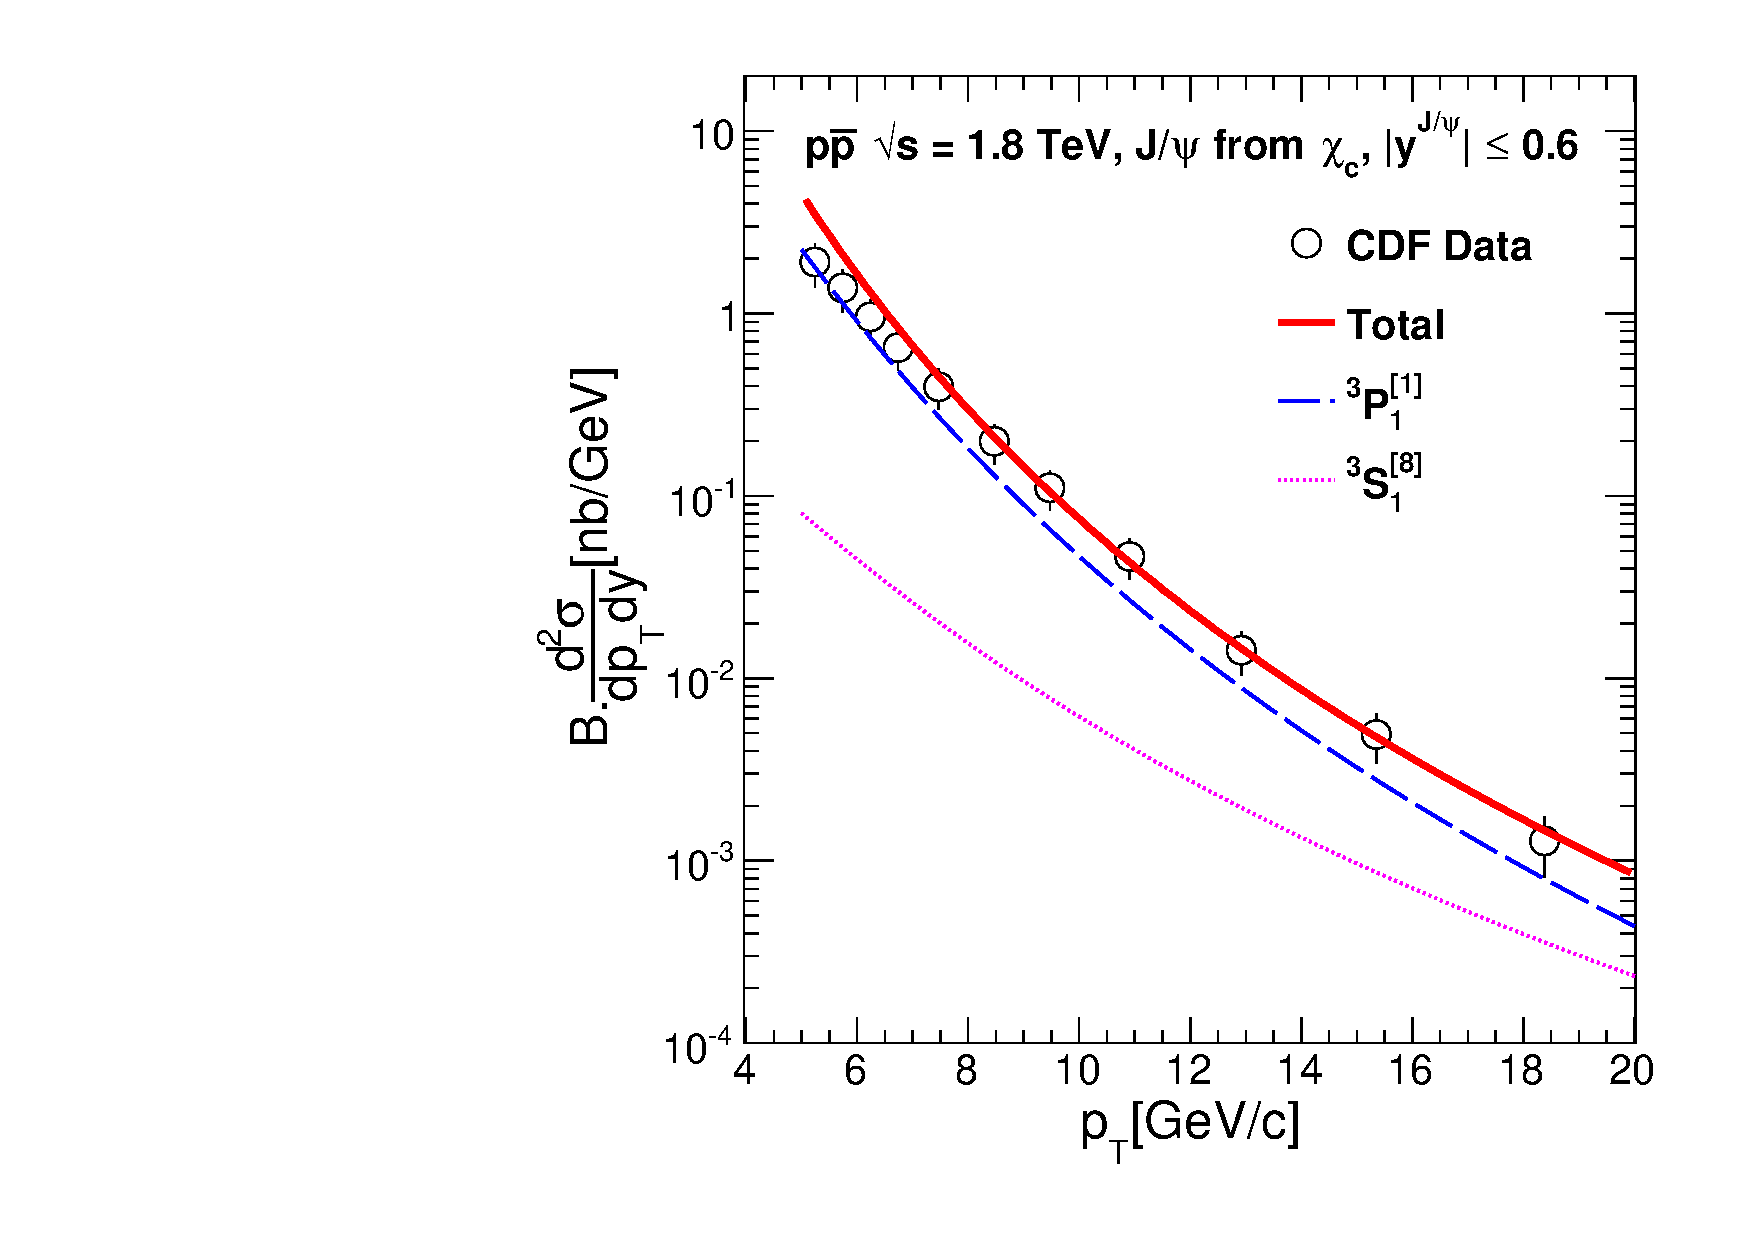
\includegraphics[width=0.49\textwidth]{Fig1_Chic1_CDF_Fit.pdf}
%\caption{(Color online) The NRQCD calculations of production cross section 
%of  $J/\psi$ from $\chi_{c1}$ and $\chi_{c2}$ decays in p+${\bar {\rm p}}$ collisions at
%$\sqrt{s}$ = 1.8 TeV as a function of transverse momentum. 
%The calculations are compared with the measured data by
%CDF experiment at Tevatron~\cite{Abe:1997yz}. The $\chi_{c}$
%color octet LDMEs are obtained by fitting this data. 
%}
%\label{Fig:LDMEChicCDF}
%\end{figure}

%CDF Abulencia:2007bra
%CMS Chatrchyan:2012ub
%ATLAS ATLAS:2014ala
%LHCb LHCb:2012af
%LHCb Aaij:2013dja


\begin{figure}
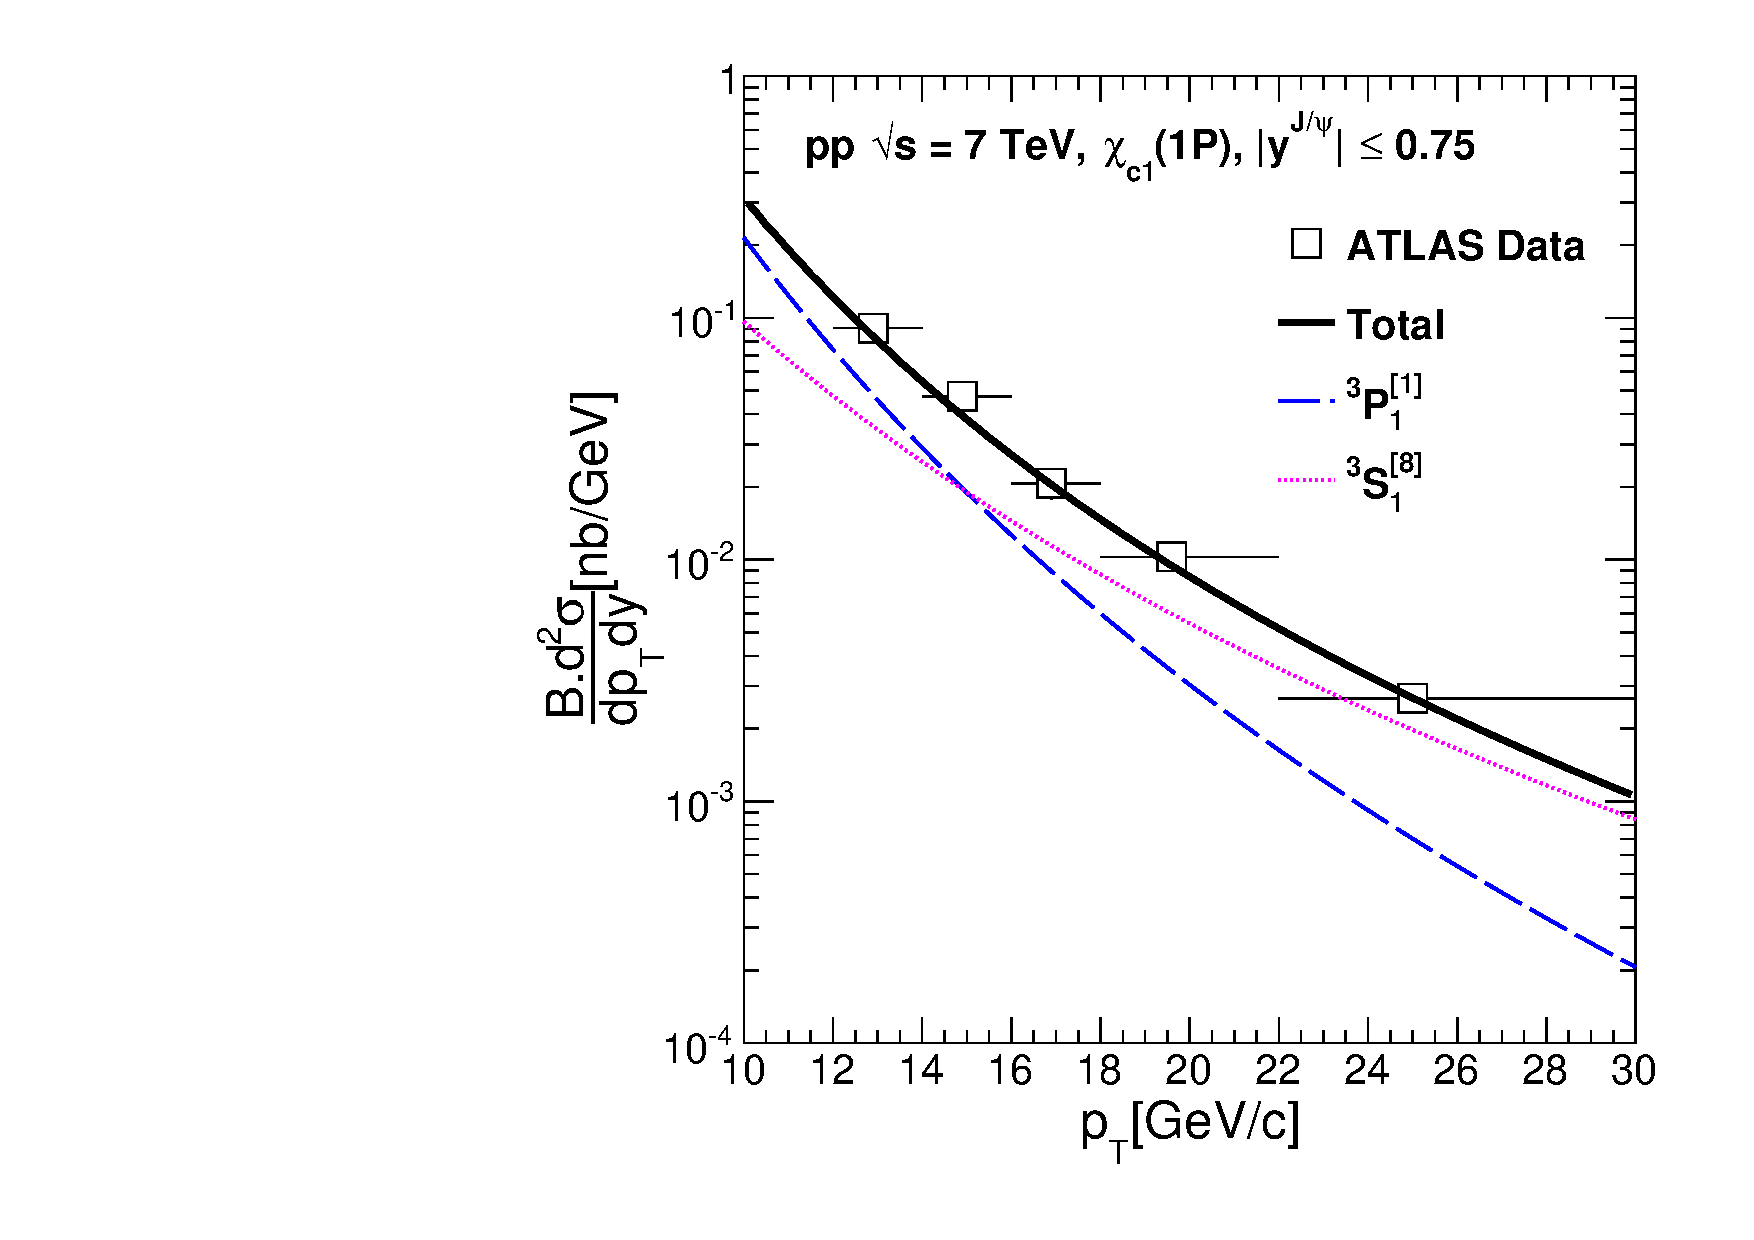
\includegraphics[width=0.49\textwidth]{Chic1_ATLAS_Fit.pdf}
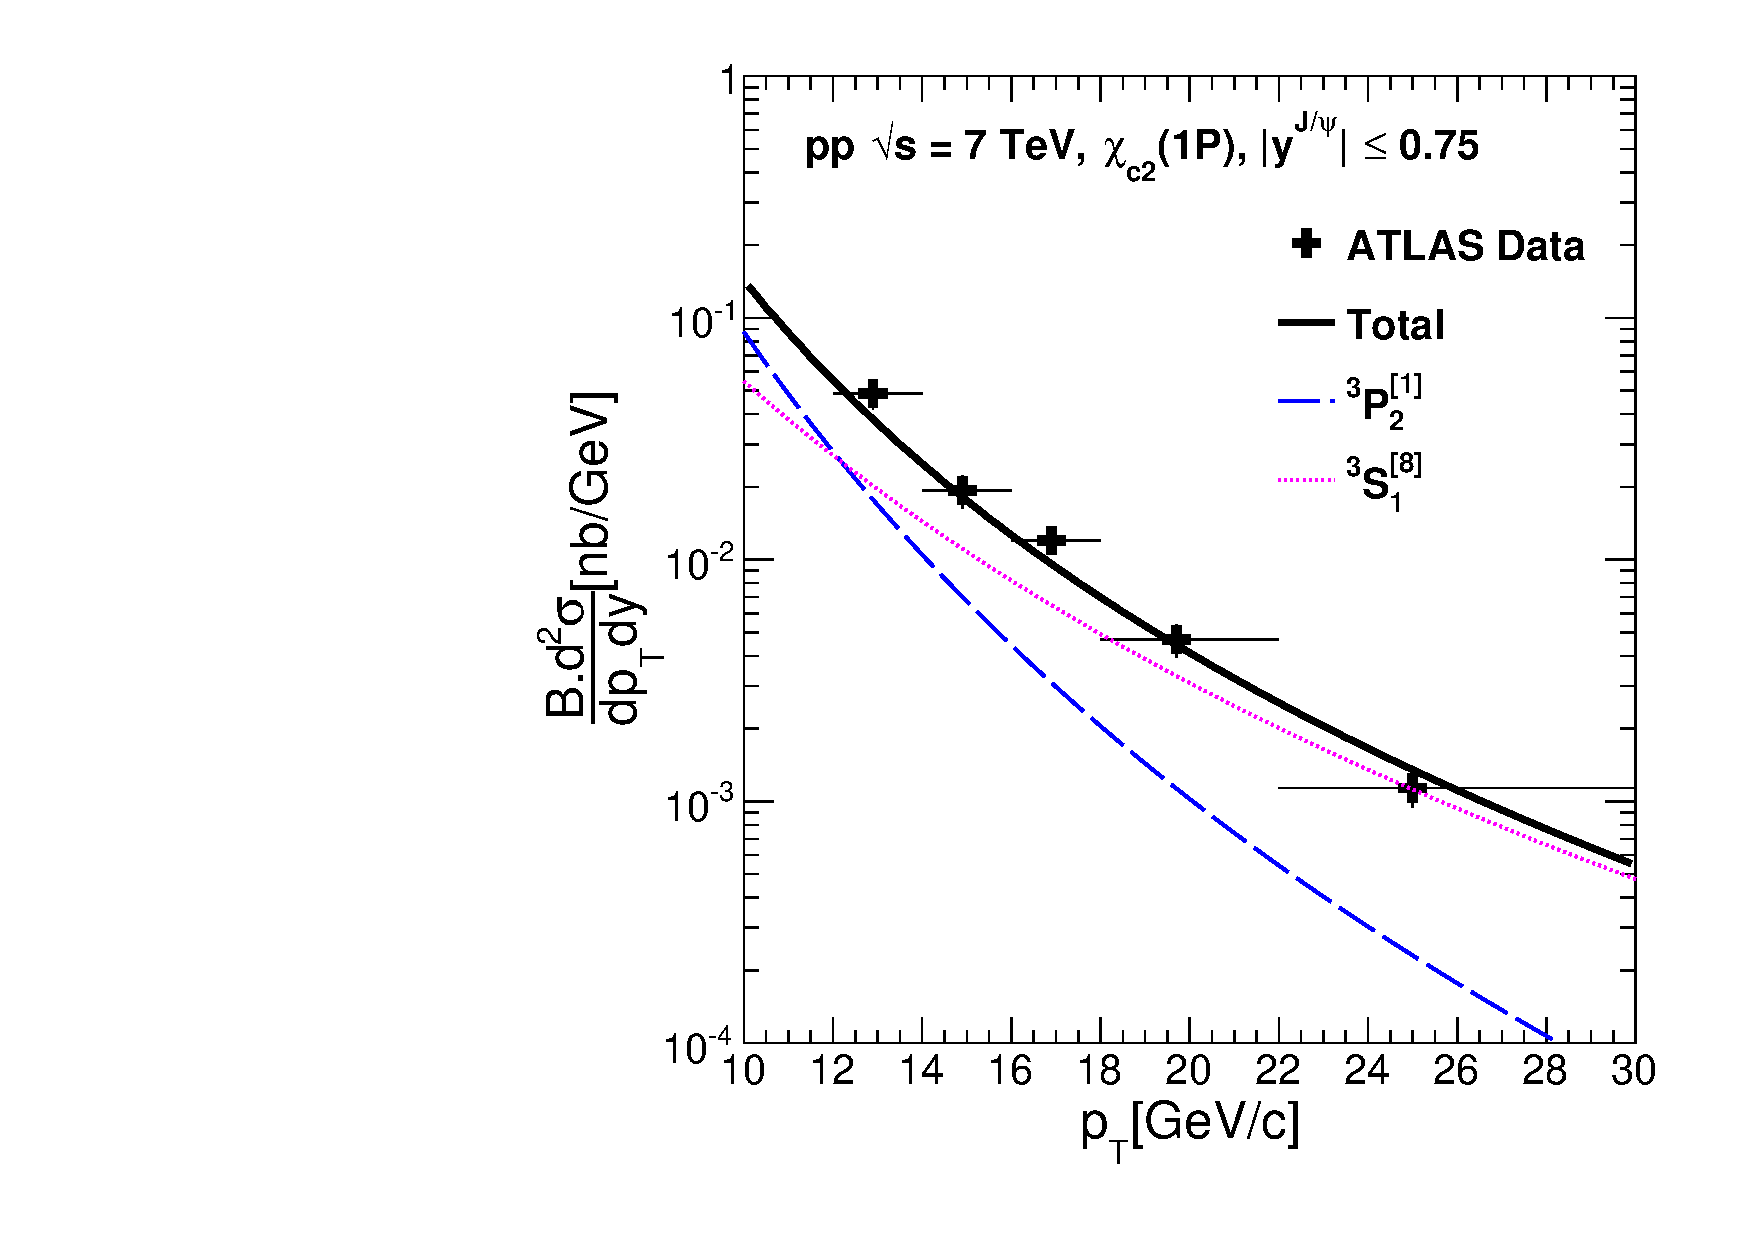
\includegraphics[width=0.49\textwidth]{Chic2_ATLAS_Fit.pdf}
\caption{(Color online) The NRQCD calculations of production cross section 
of  $\chi_{c1}$ and $\chi_{c2}$ in p+p collisions at
$\sqrt{s}$ = 7.0 TeV as a function of transverse momentum. 
The Calculations are compared with the measured data by
ATLAS experiment at LHC~\cite{ATLAS:2014ala}. The $\chi_{c}$
color octet LDMEs are obtained by fitting this data. 
}
\label{Fig:LDMEChicCDF}
\end{figure}

\begin{figure}
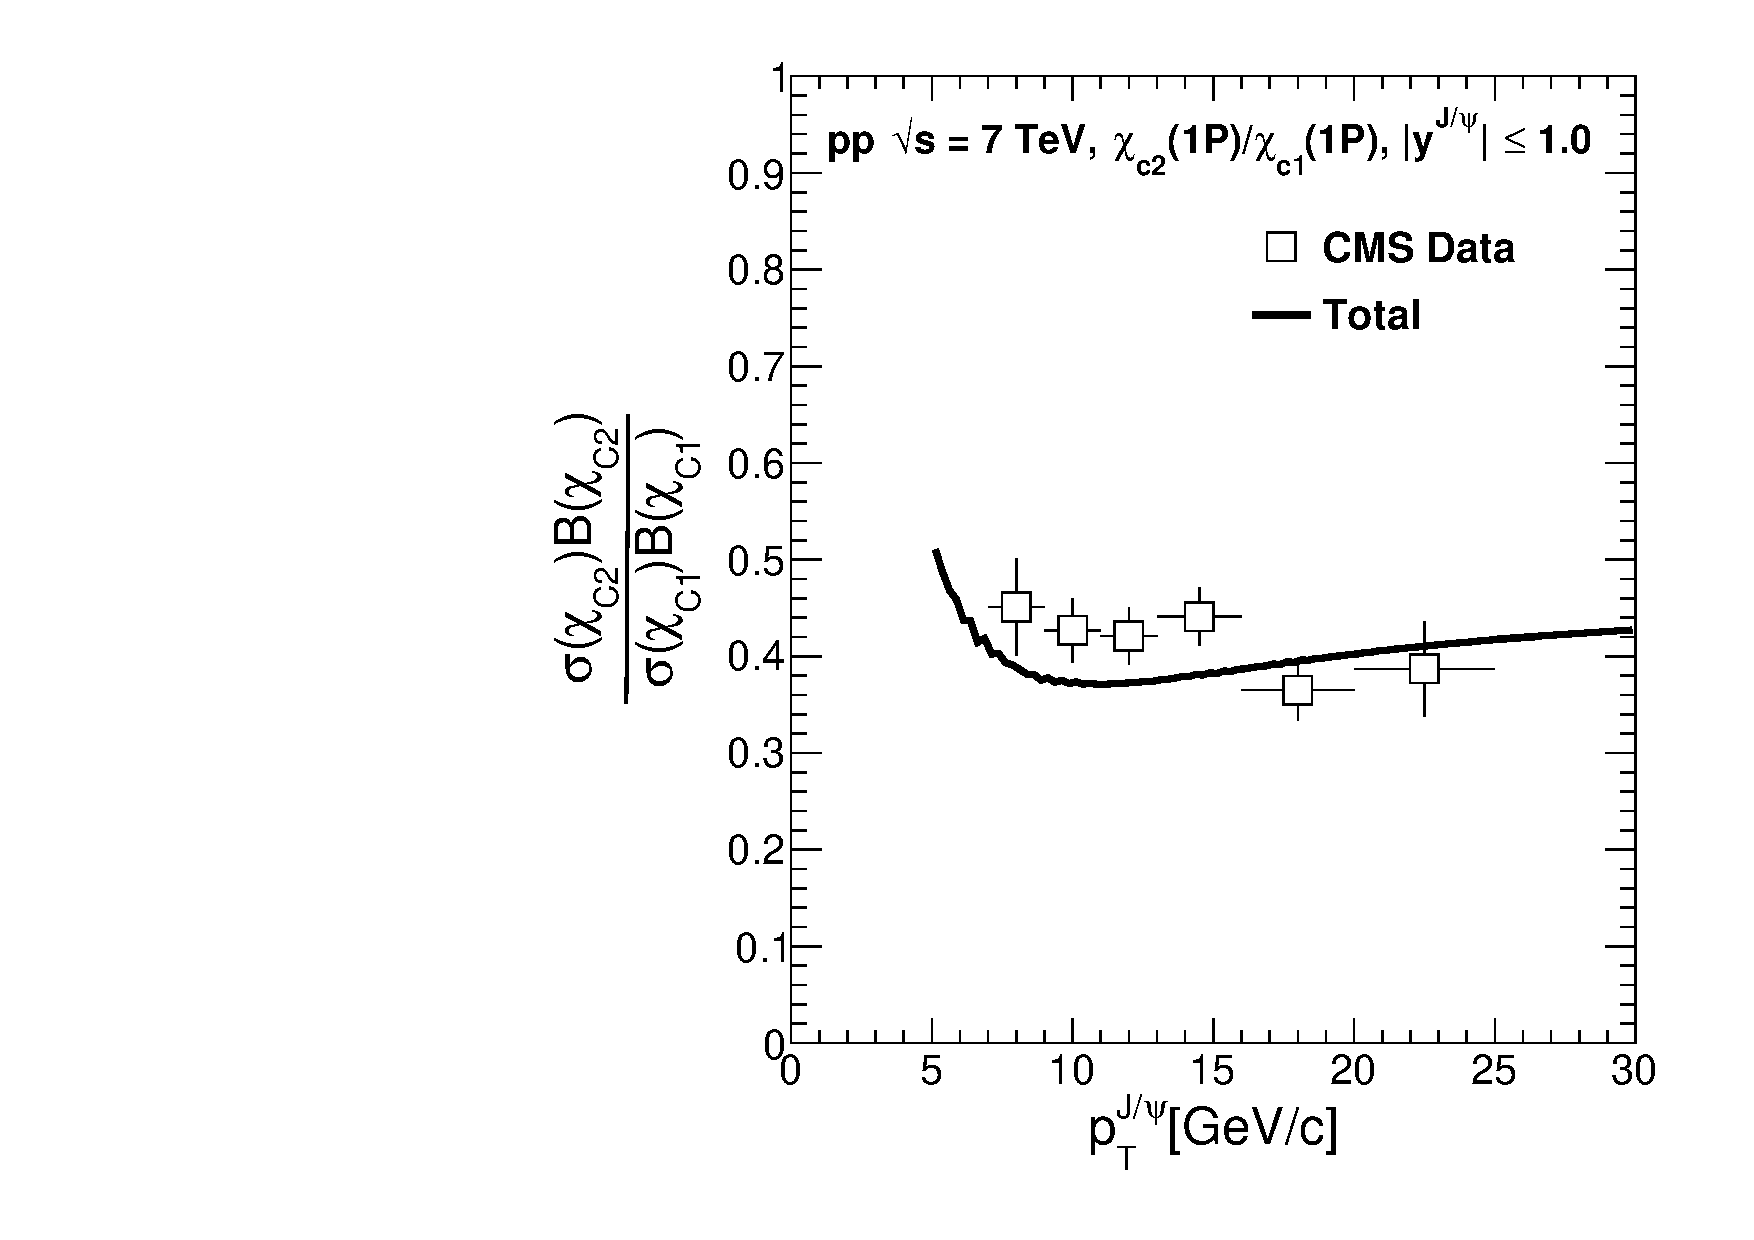
\includegraphics[width=0.49\textwidth]{Chic2Chic1_CMS_Fit.pdf}
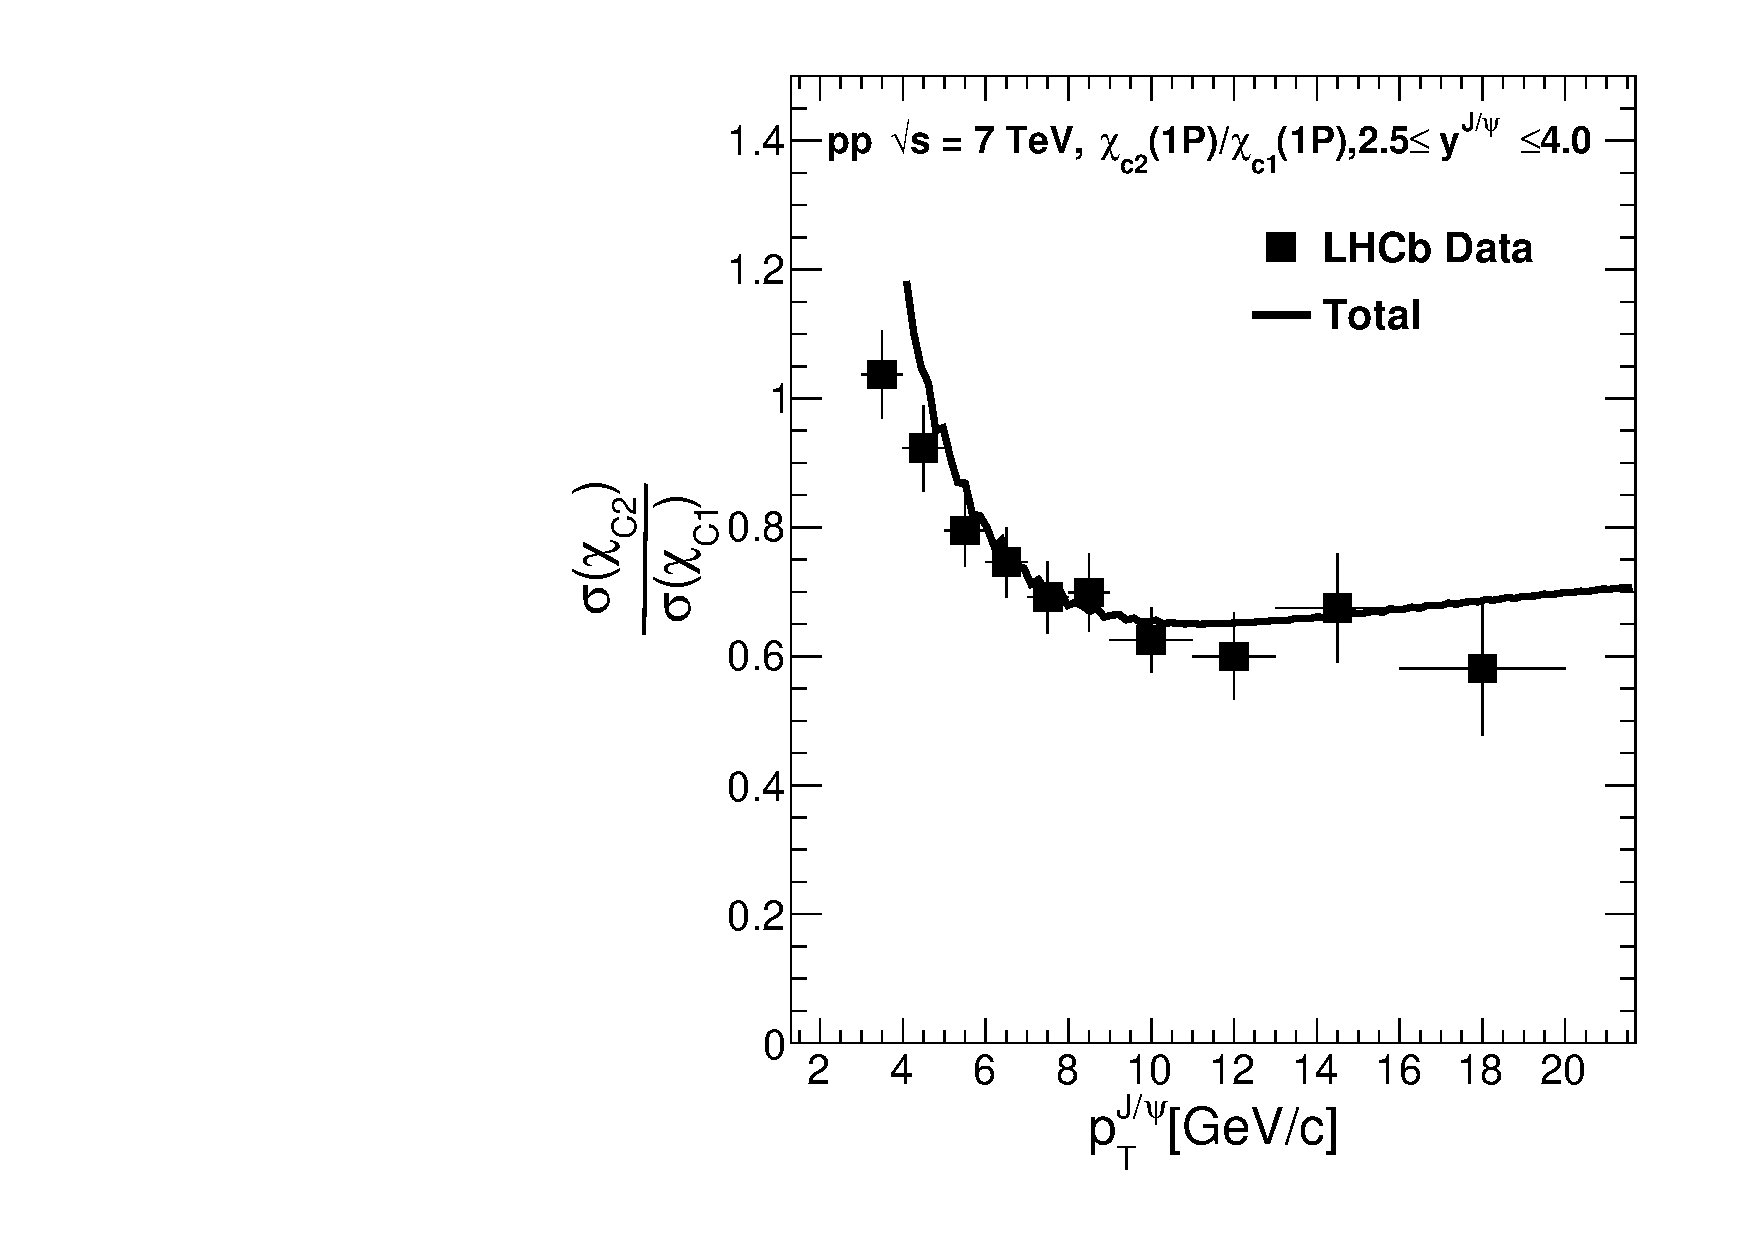
\includegraphics[width=0.49\textwidth]{Chic2Chic1_LHCb_Fit.pdf}
\caption{(Color online) The NRQCD calculations of production cross section ratios 
of  $\chi_{c2}$ and $\chi_{c1}$ in p+p collisions at
$\sqrt{s}$ = 7.0 TeV as a function of transverse momentum. 
The Calculations are compared with the measured data by
CMS and LHCb experiments at LHC~\cite{Chatrchyan:2012ub,Aaij:2013dja}. The $\chi_{c}$
color octet LDMEs are obtained by fitting this data. 
}
\label{Fig:LDMEChicCDF}
\end{figure}
















\begin{figure}
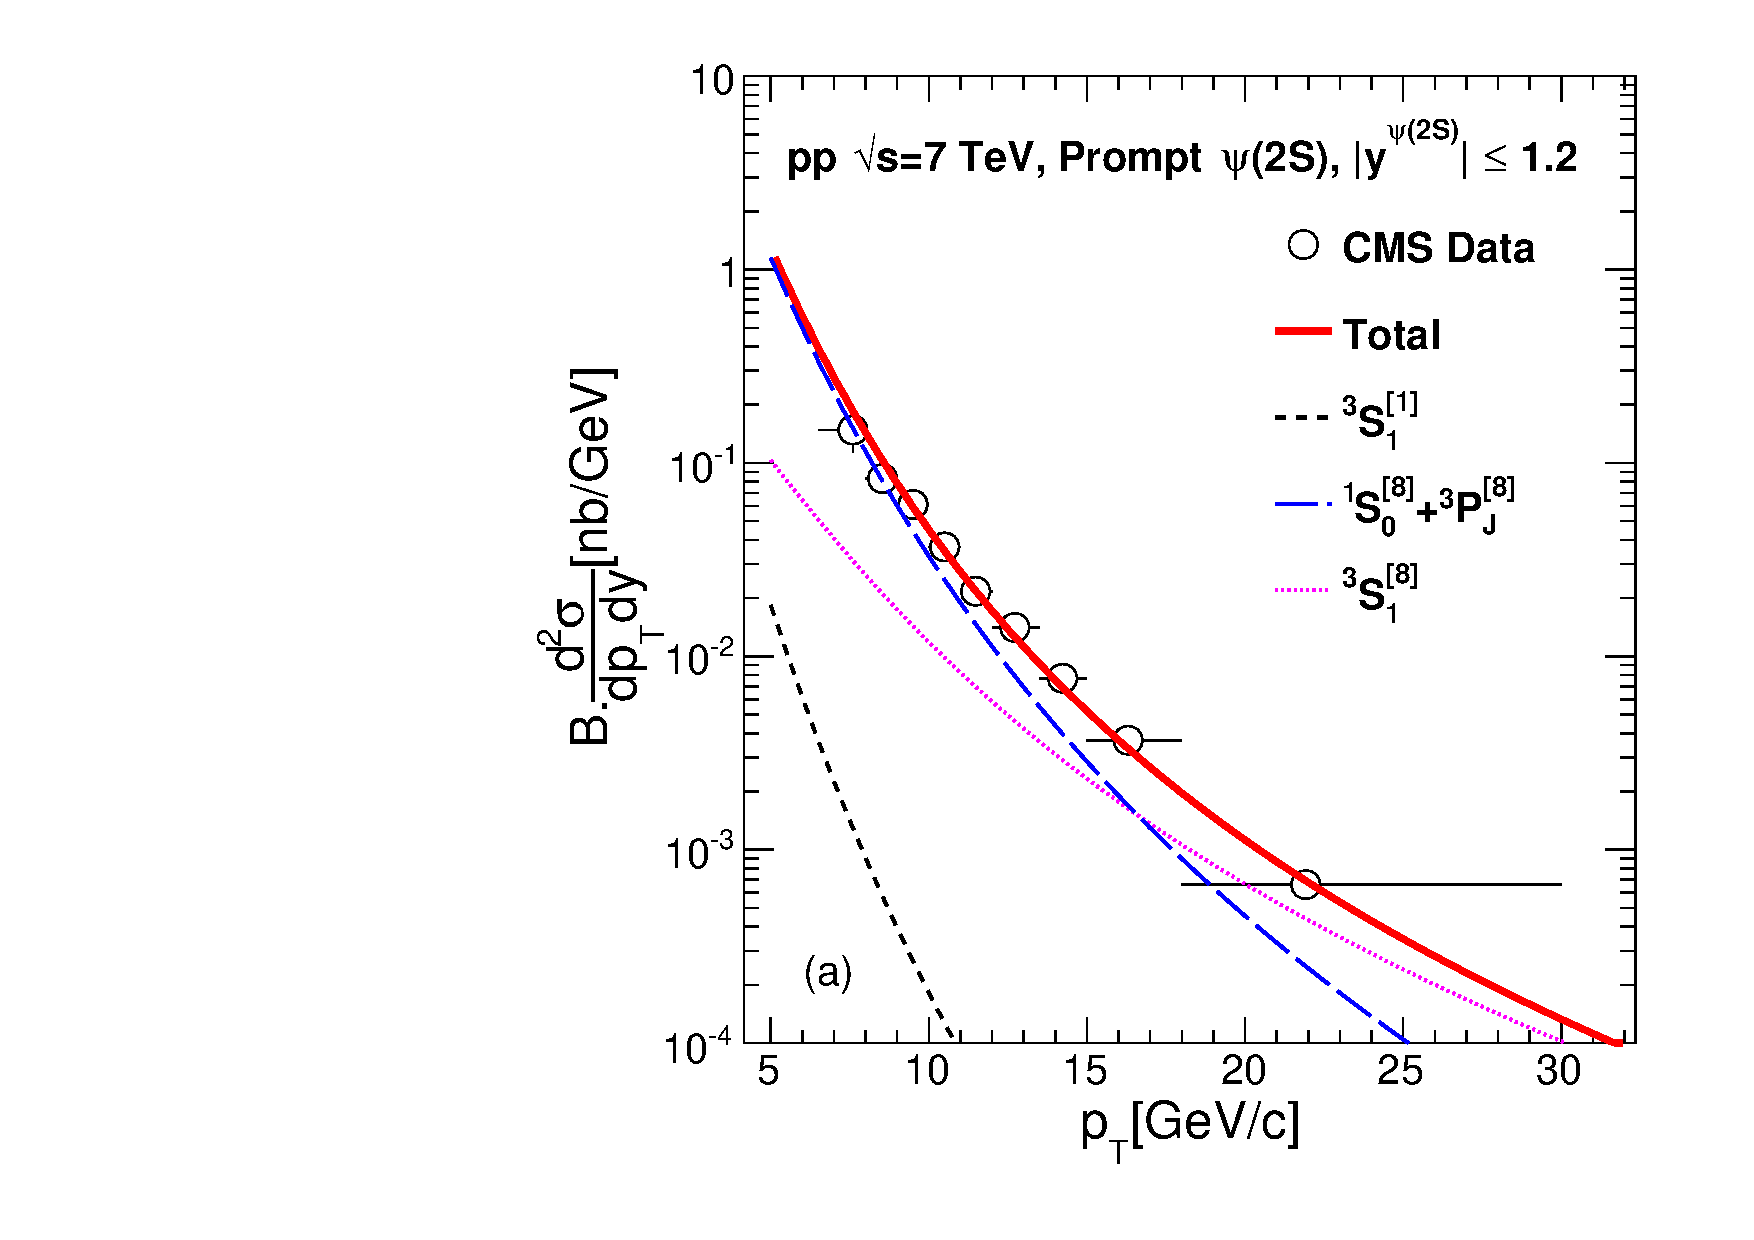
\includegraphics[width=0.49\textwidth]{Psi2S_CMS_LowPt.pdf}
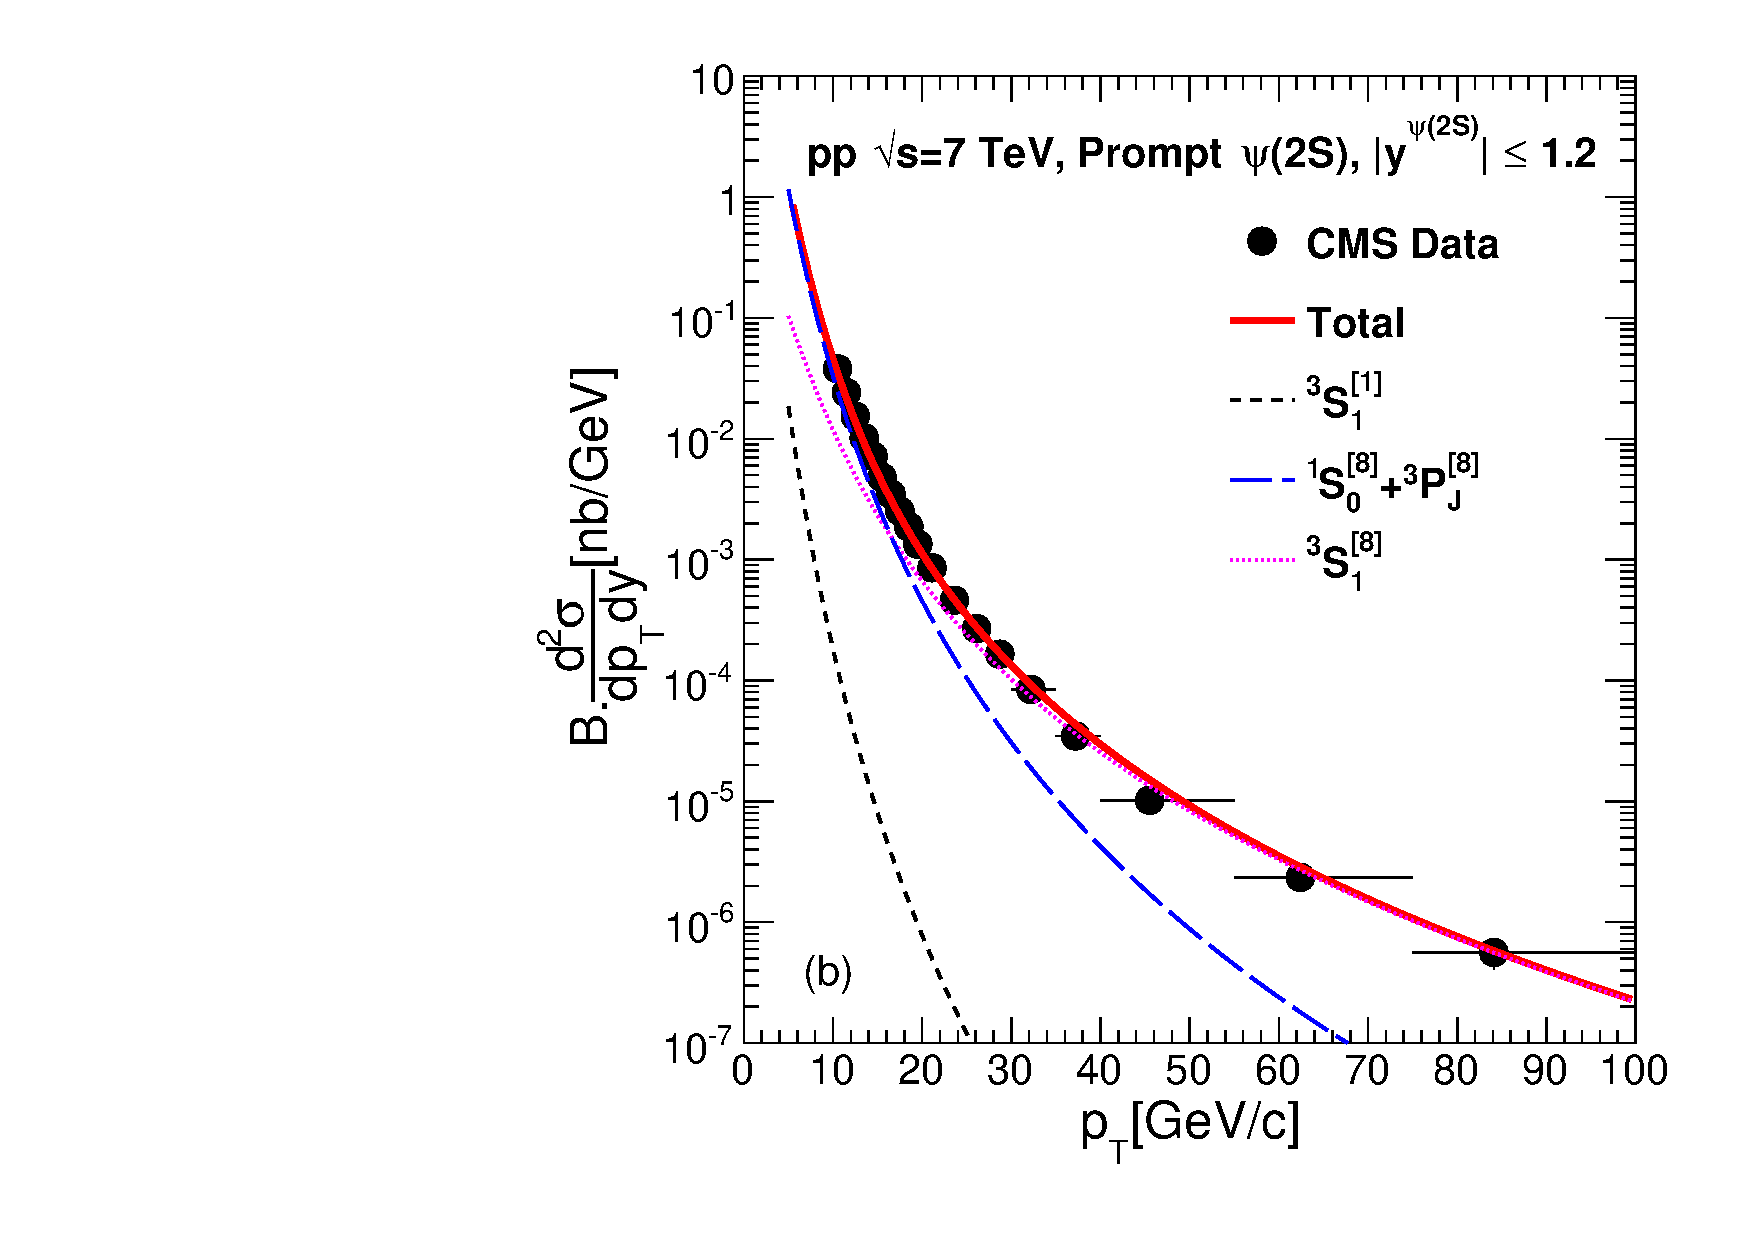
\includegraphics[width=0.49\textwidth]{Psi2S_CMS_HighPt.pdf}
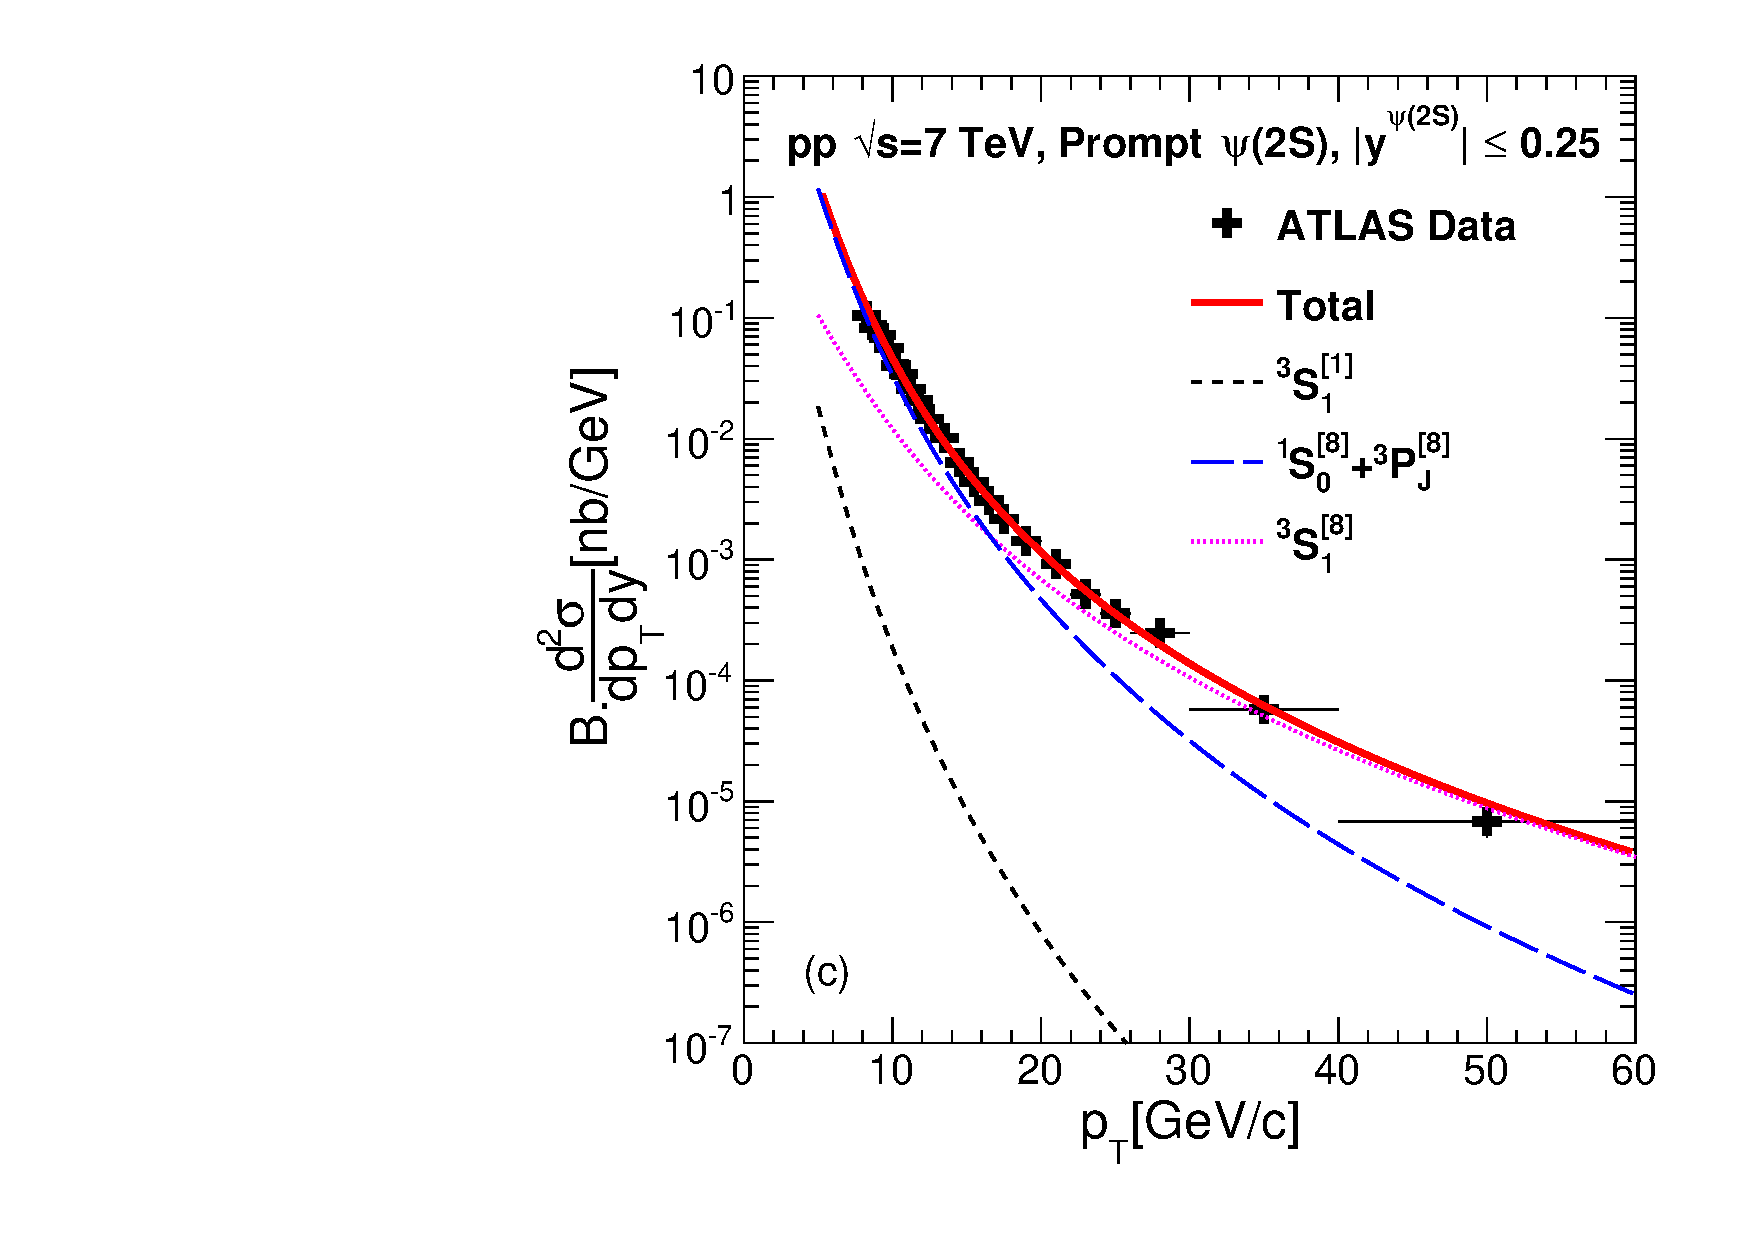
\includegraphics[width=0.49\textwidth]{Psi2S_ATLAS.pdf}
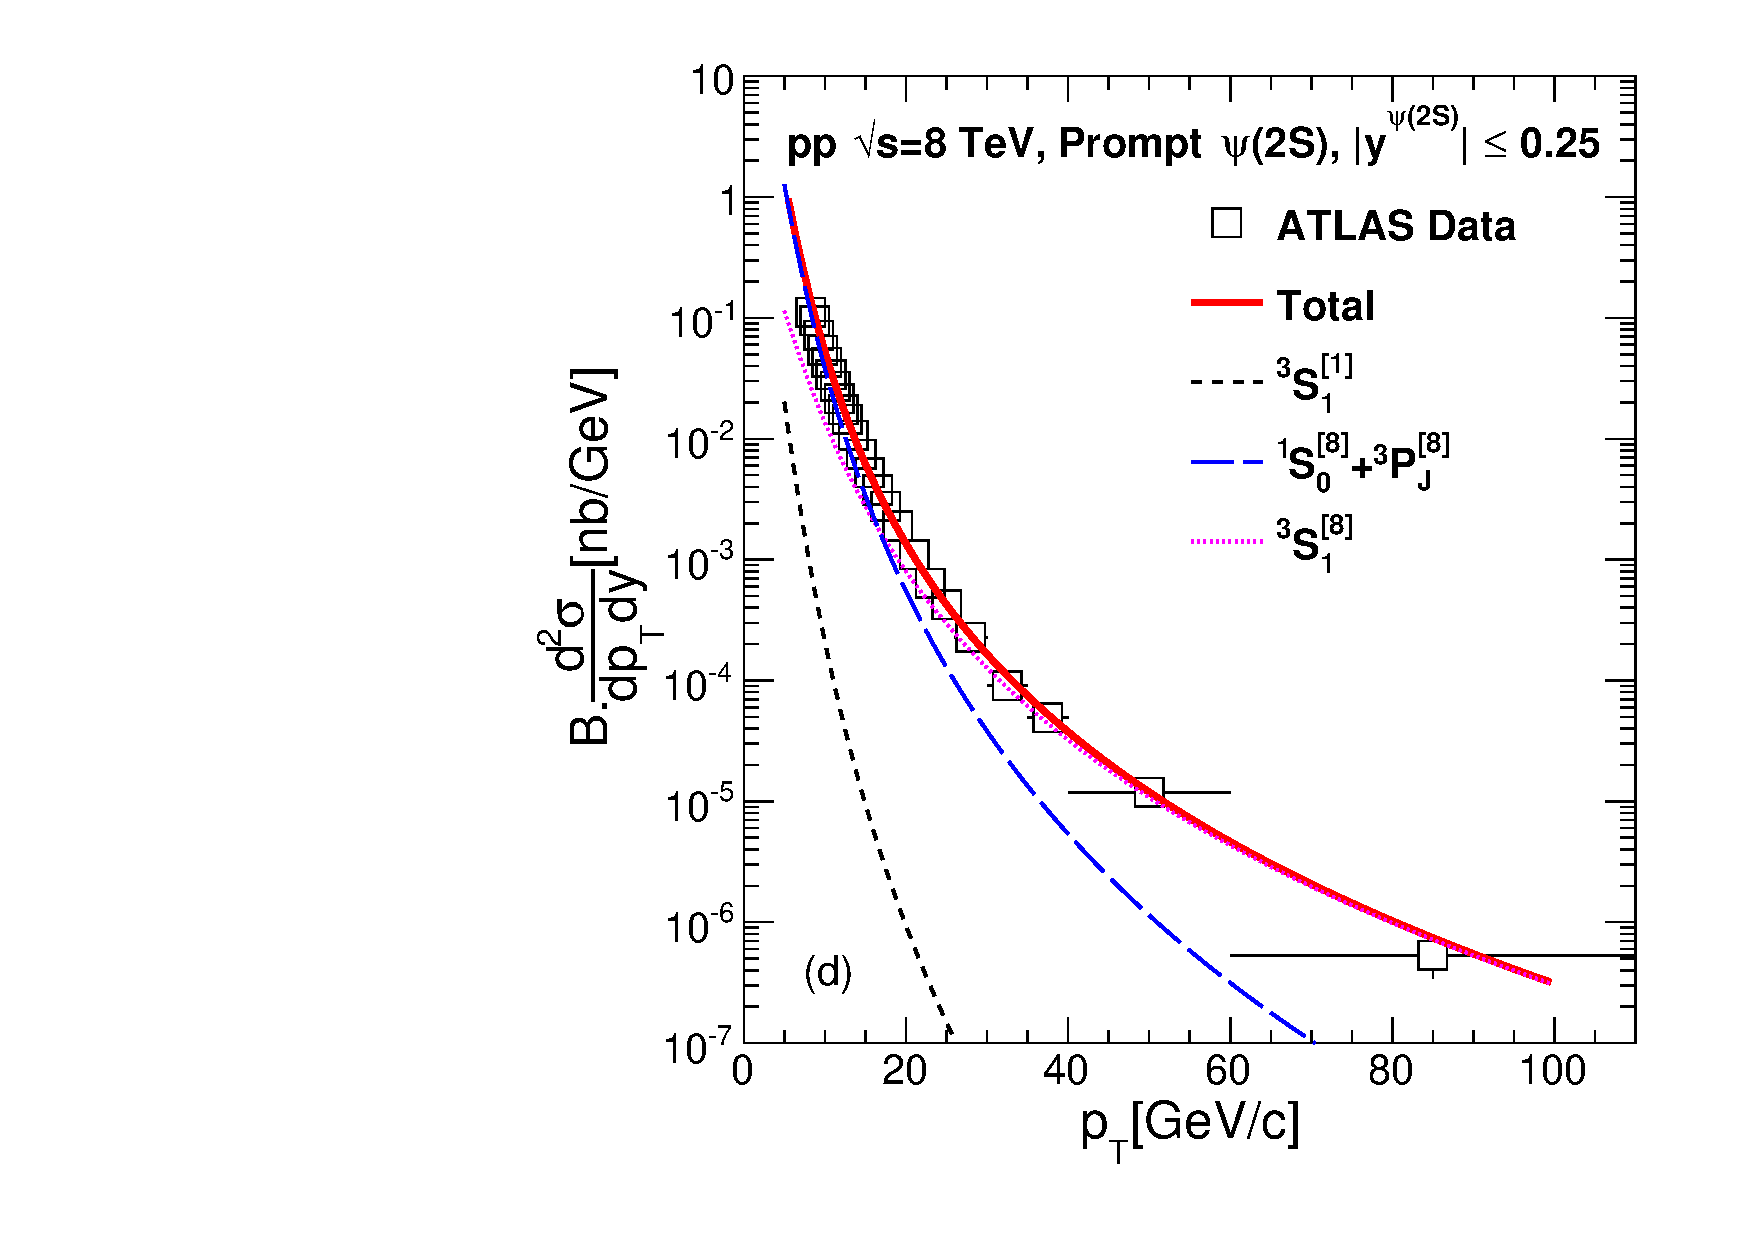
\includegraphics[width=0.49\textwidth]{Psi2S_ATLAS_8TeV.pdf}
\caption{(Color online) 
  The NRQCD calculations of production cross section of $\psi$(2S) in p+p collisions 
as a function of transverse momentum compared with the measured data at LHC 
 (a) CMS data at $\sqrt{s}$ = 7 TeV~\cite{Chatrchyan:2011kc} 
 (b) CMS data at $\sqrt{s}$ = 7 TeV~\cite{Khachatryan:2015rra} 
 (c) ATLAS data at $\sqrt{s}$ = 7 TeV and
 (d) ATLAS data at $\sqrt{s}$ = 8 TeV~\cite{Aad:2015duc}. 
 The LDMEs are obtained by a combined fit of the LHC and Tevatron data.
}
\label{Fig:LDMEPsi2S}
\end{figure}

\begin{figure}
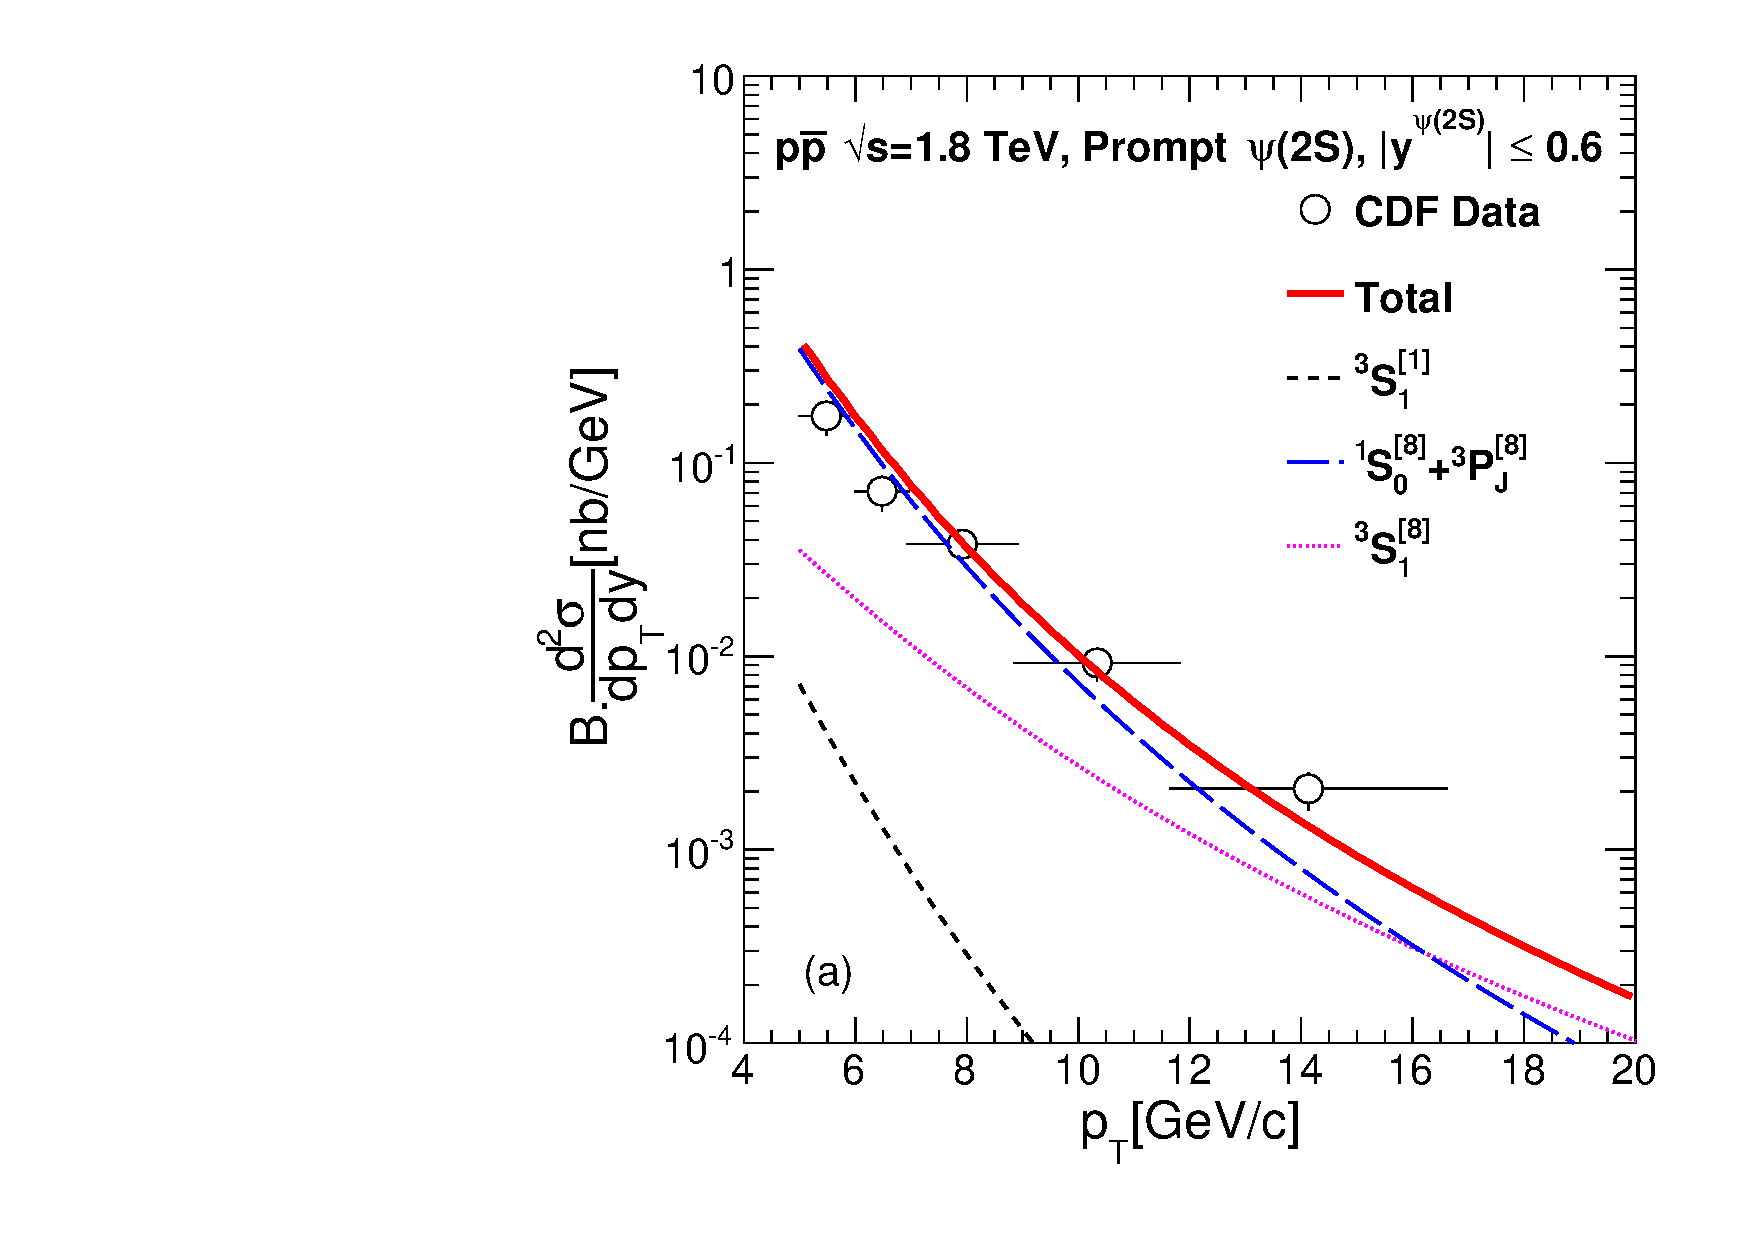
\includegraphics[width=0.49\textwidth]{Psi2S_CDF_180TeV.pdf}
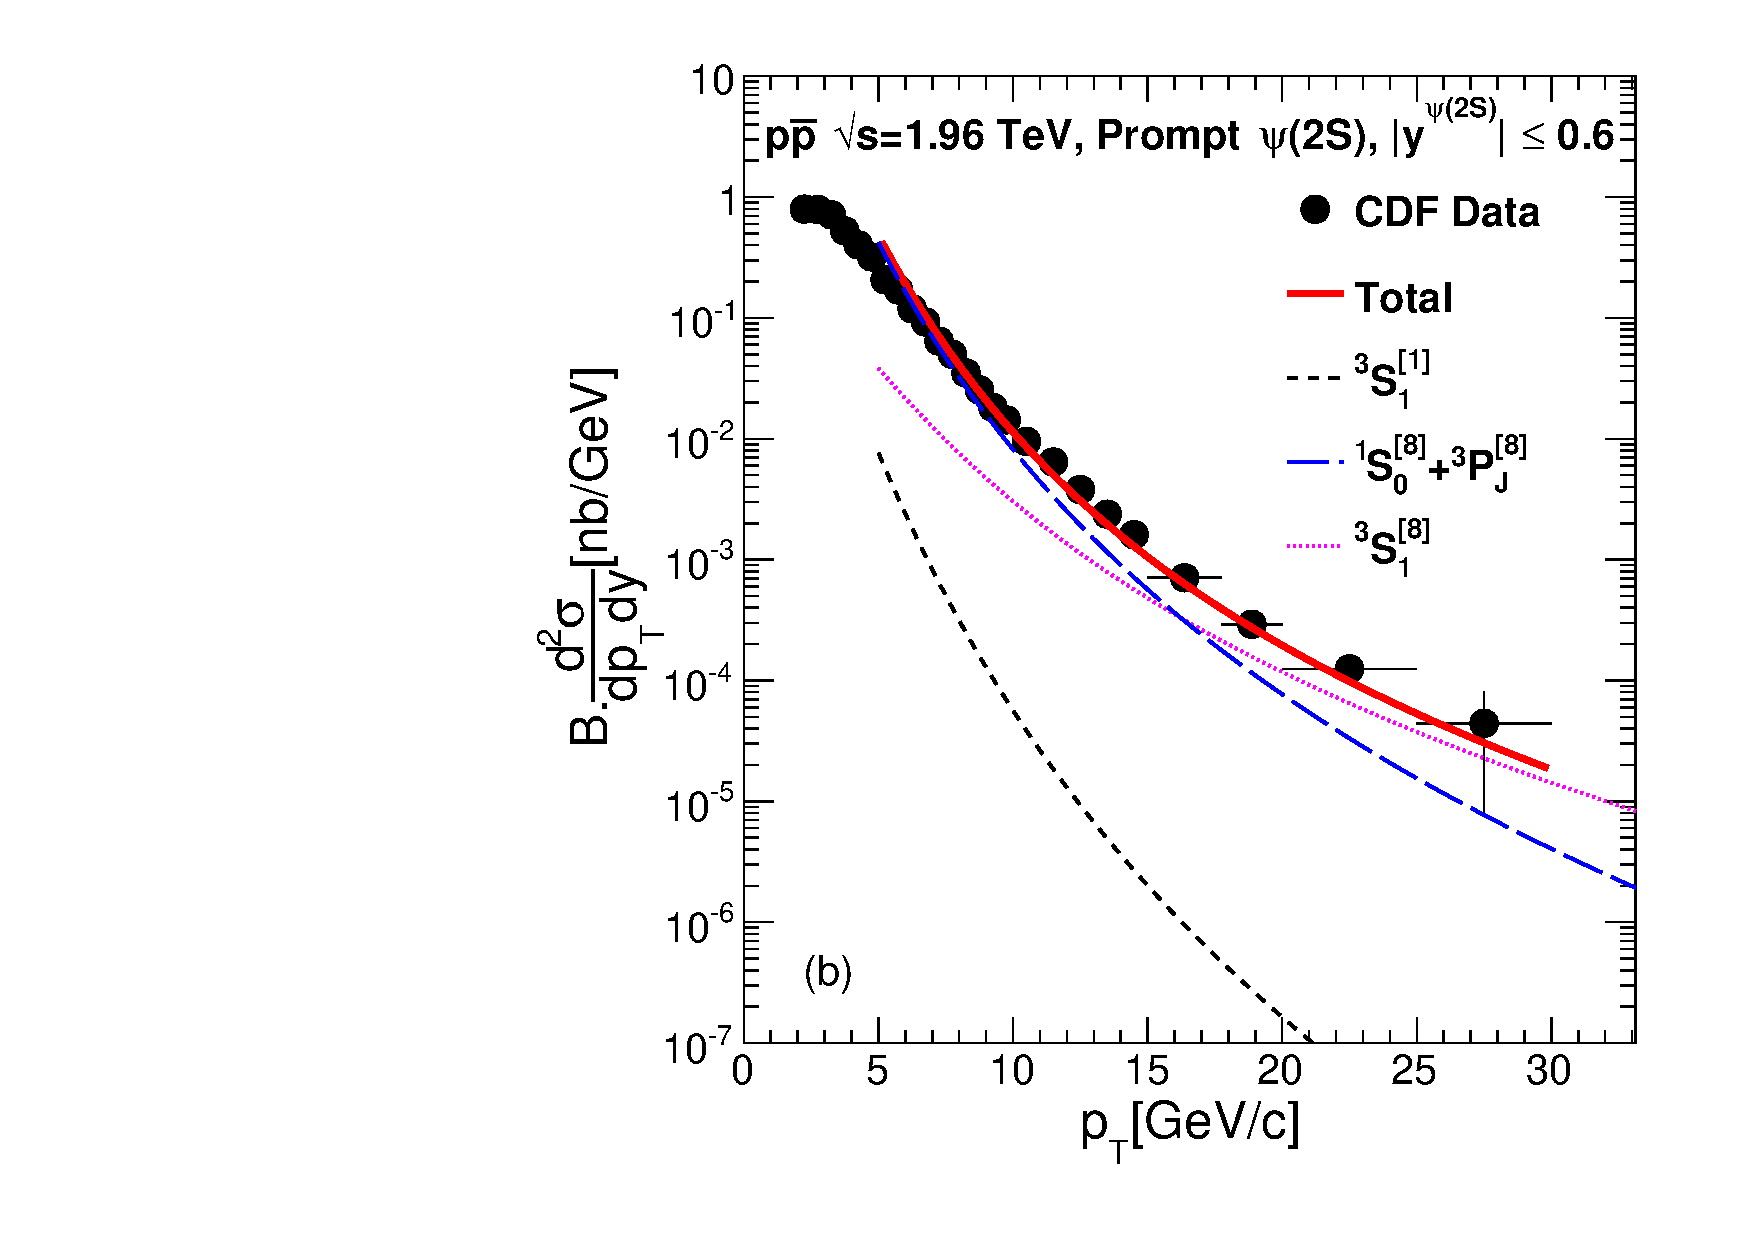
\includegraphics[width=0.49\textwidth]{Psi2S_CDF_196TeV.pdf}
\caption{(Color online) The NRQCD calculations of production cross section 
of $\psi$(2S) in p+${\bar {\rm p}}$ collisions as a function of transverse momentum compared 
with the measured data at Tevatron 
(a) CDF data at $\sqrt{s}$ = 1.8 TeV~\cite{Abe:1997jz} and
(b) CDF data at $\sqrt{s}$ = 1.96 TeV~\cite{Acosta:2004yw}. 
The LDMEs are obtained by a combined fit of the Tevatron and
LHC data.
}
\label{Fig:LDMEPsi2SCDF}
\end{figure}








\begin{figure}
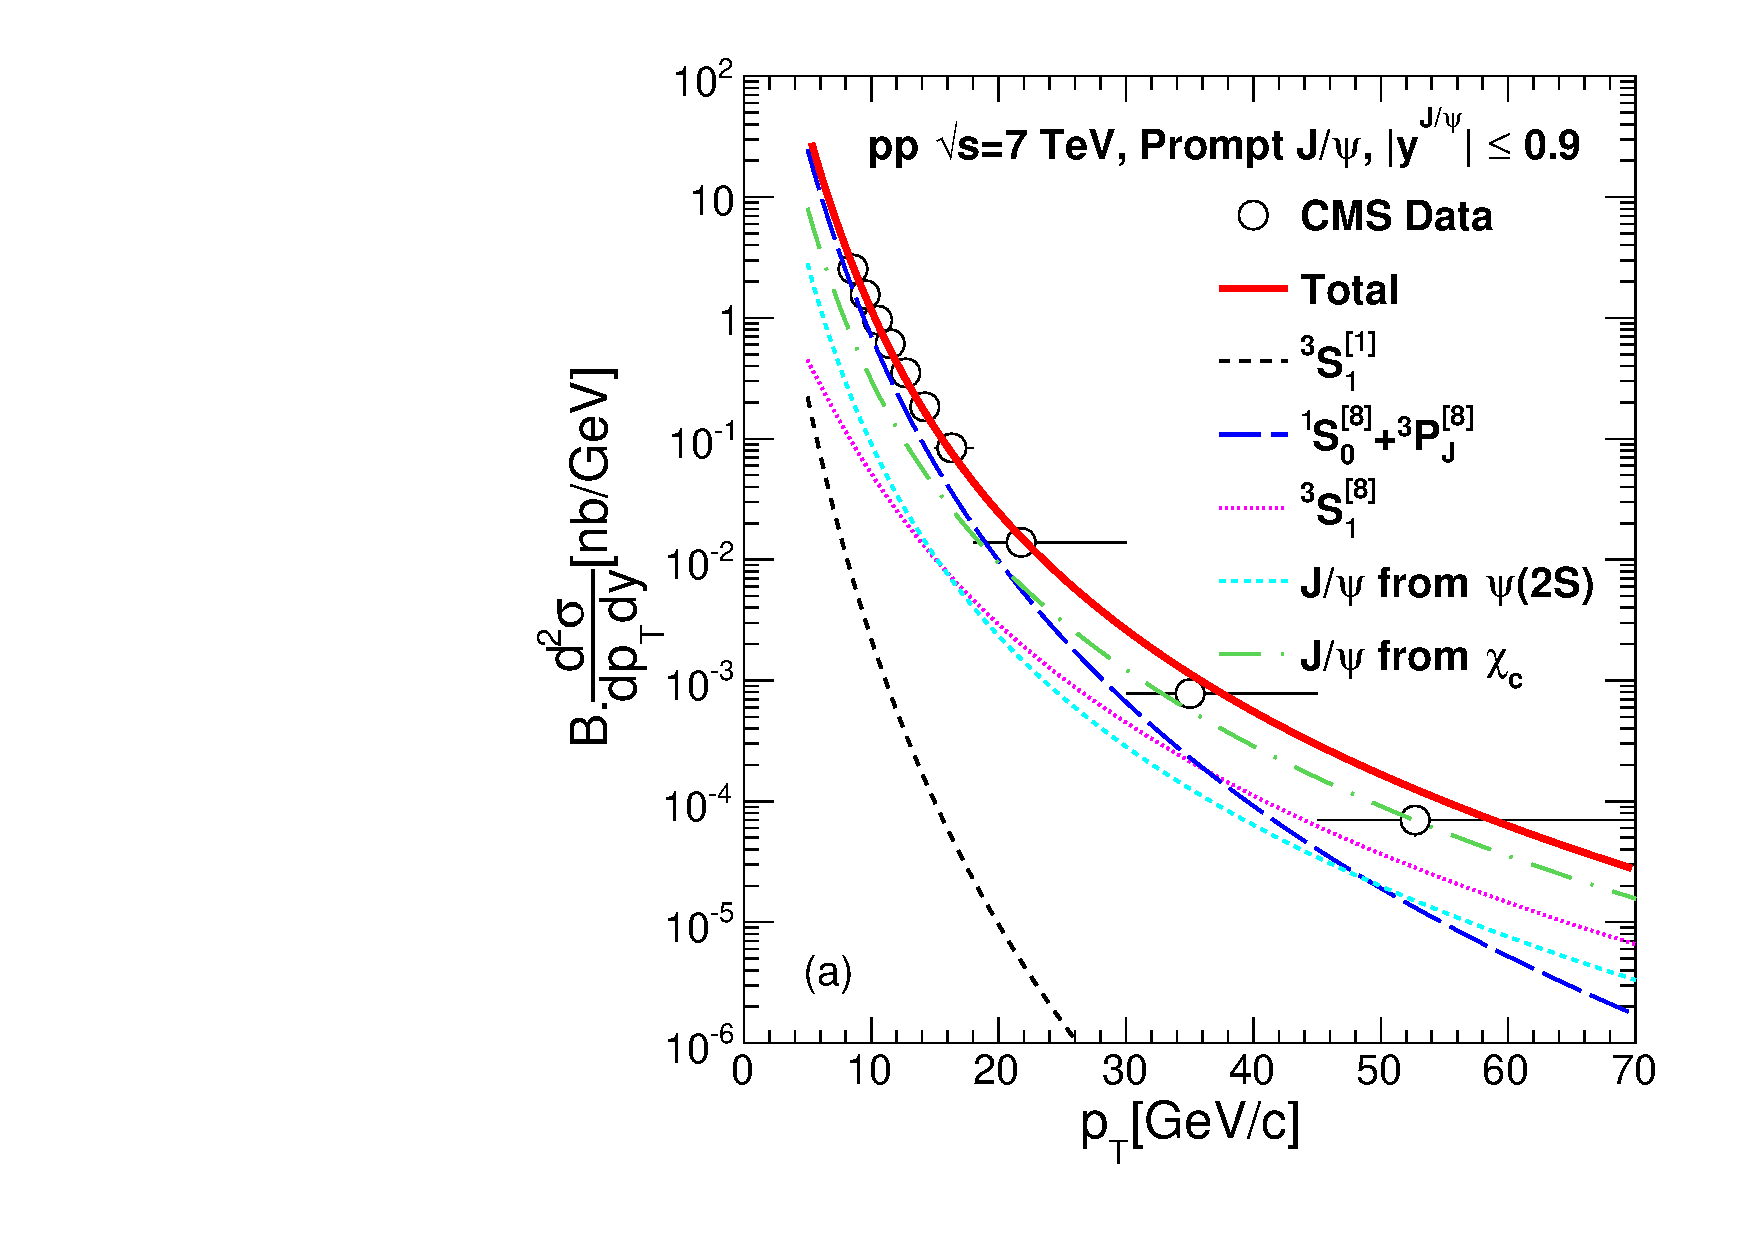
\includegraphics[width=0.49\textwidth]{CMS_New_D2NDPtDy_PromptJPsi_Y0009_Pt.pdf}
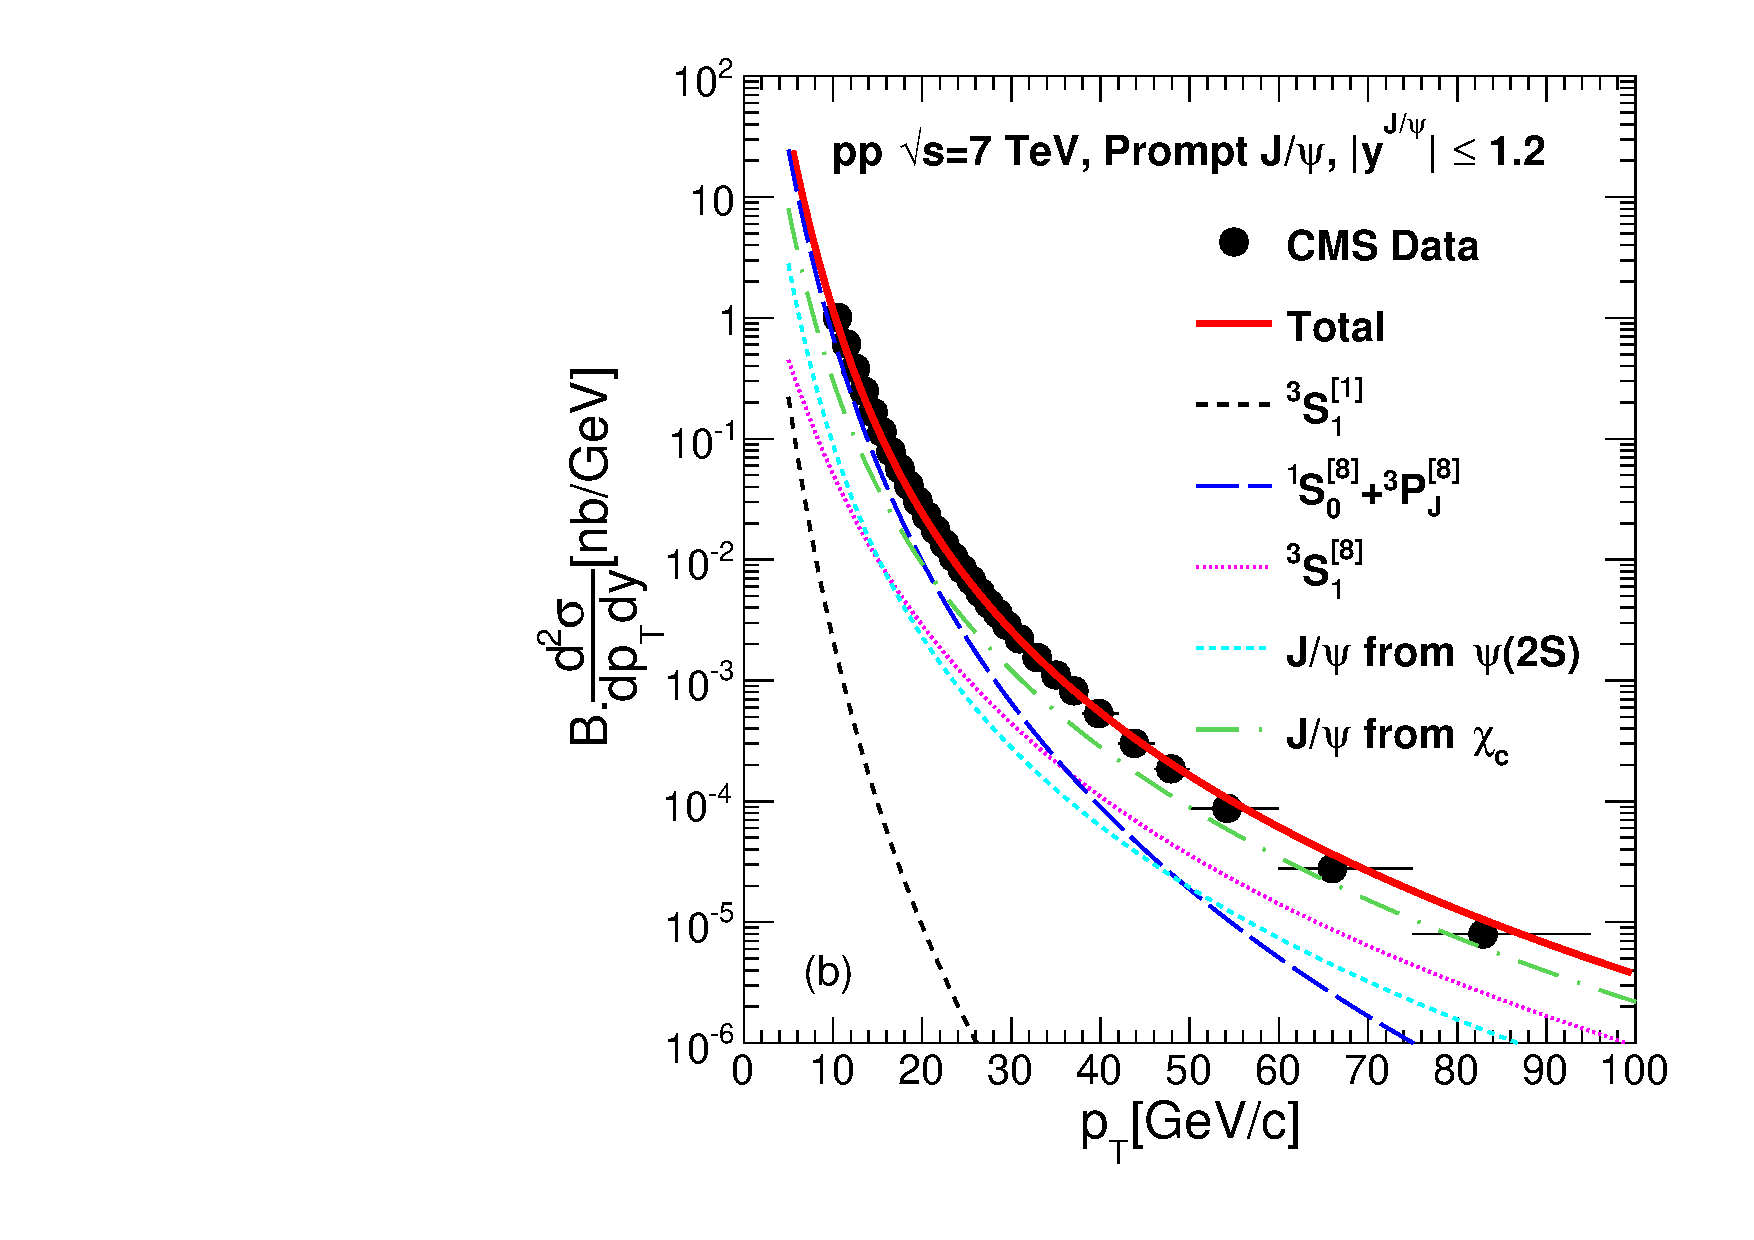
\includegraphics[width=0.49\textwidth]{CMS_Latest_D2NDPtDy_PromptJPsi_Y0012_Pt.pdf}
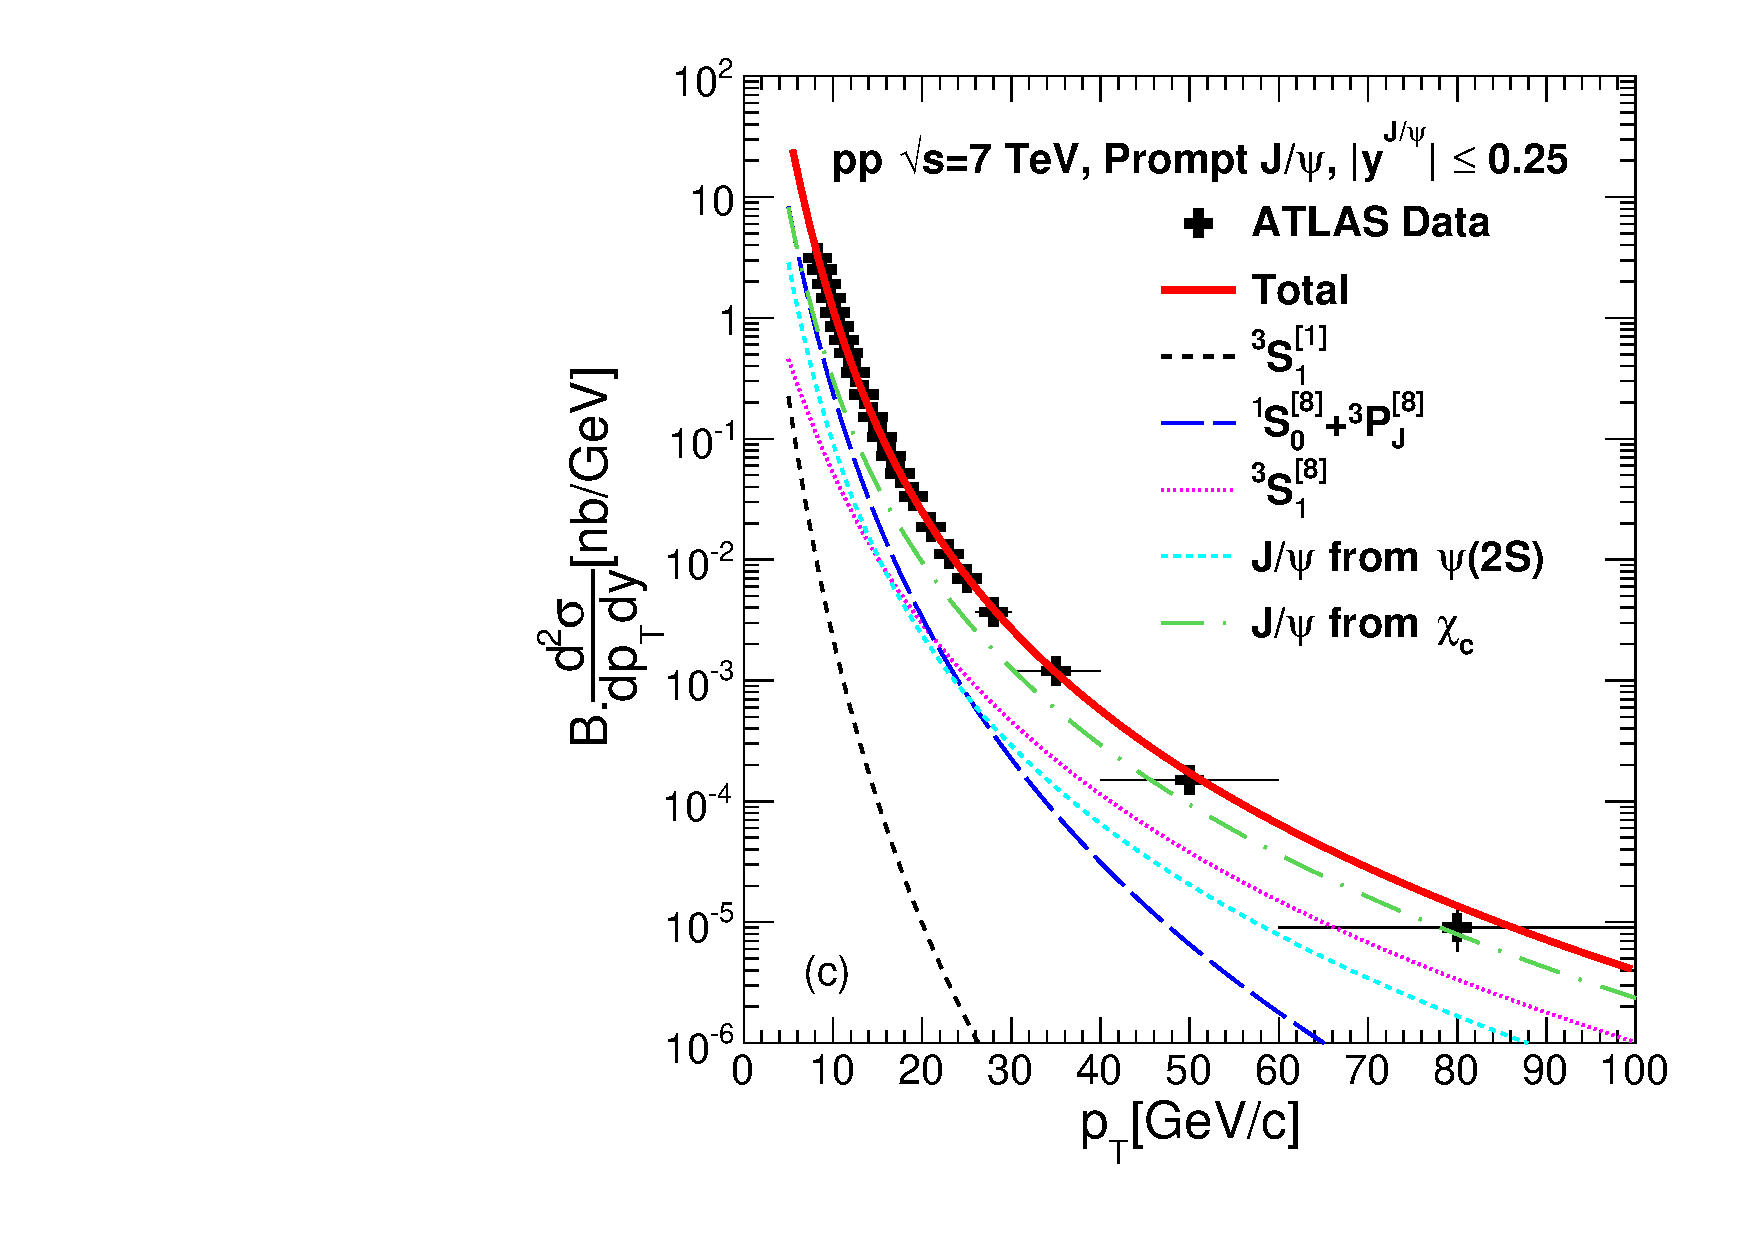
\includegraphics[width=0.49\textwidth]{ATLAS_7TeV_D2NDPtDy_PromptJPsi_Y0025_Pt.pdf}
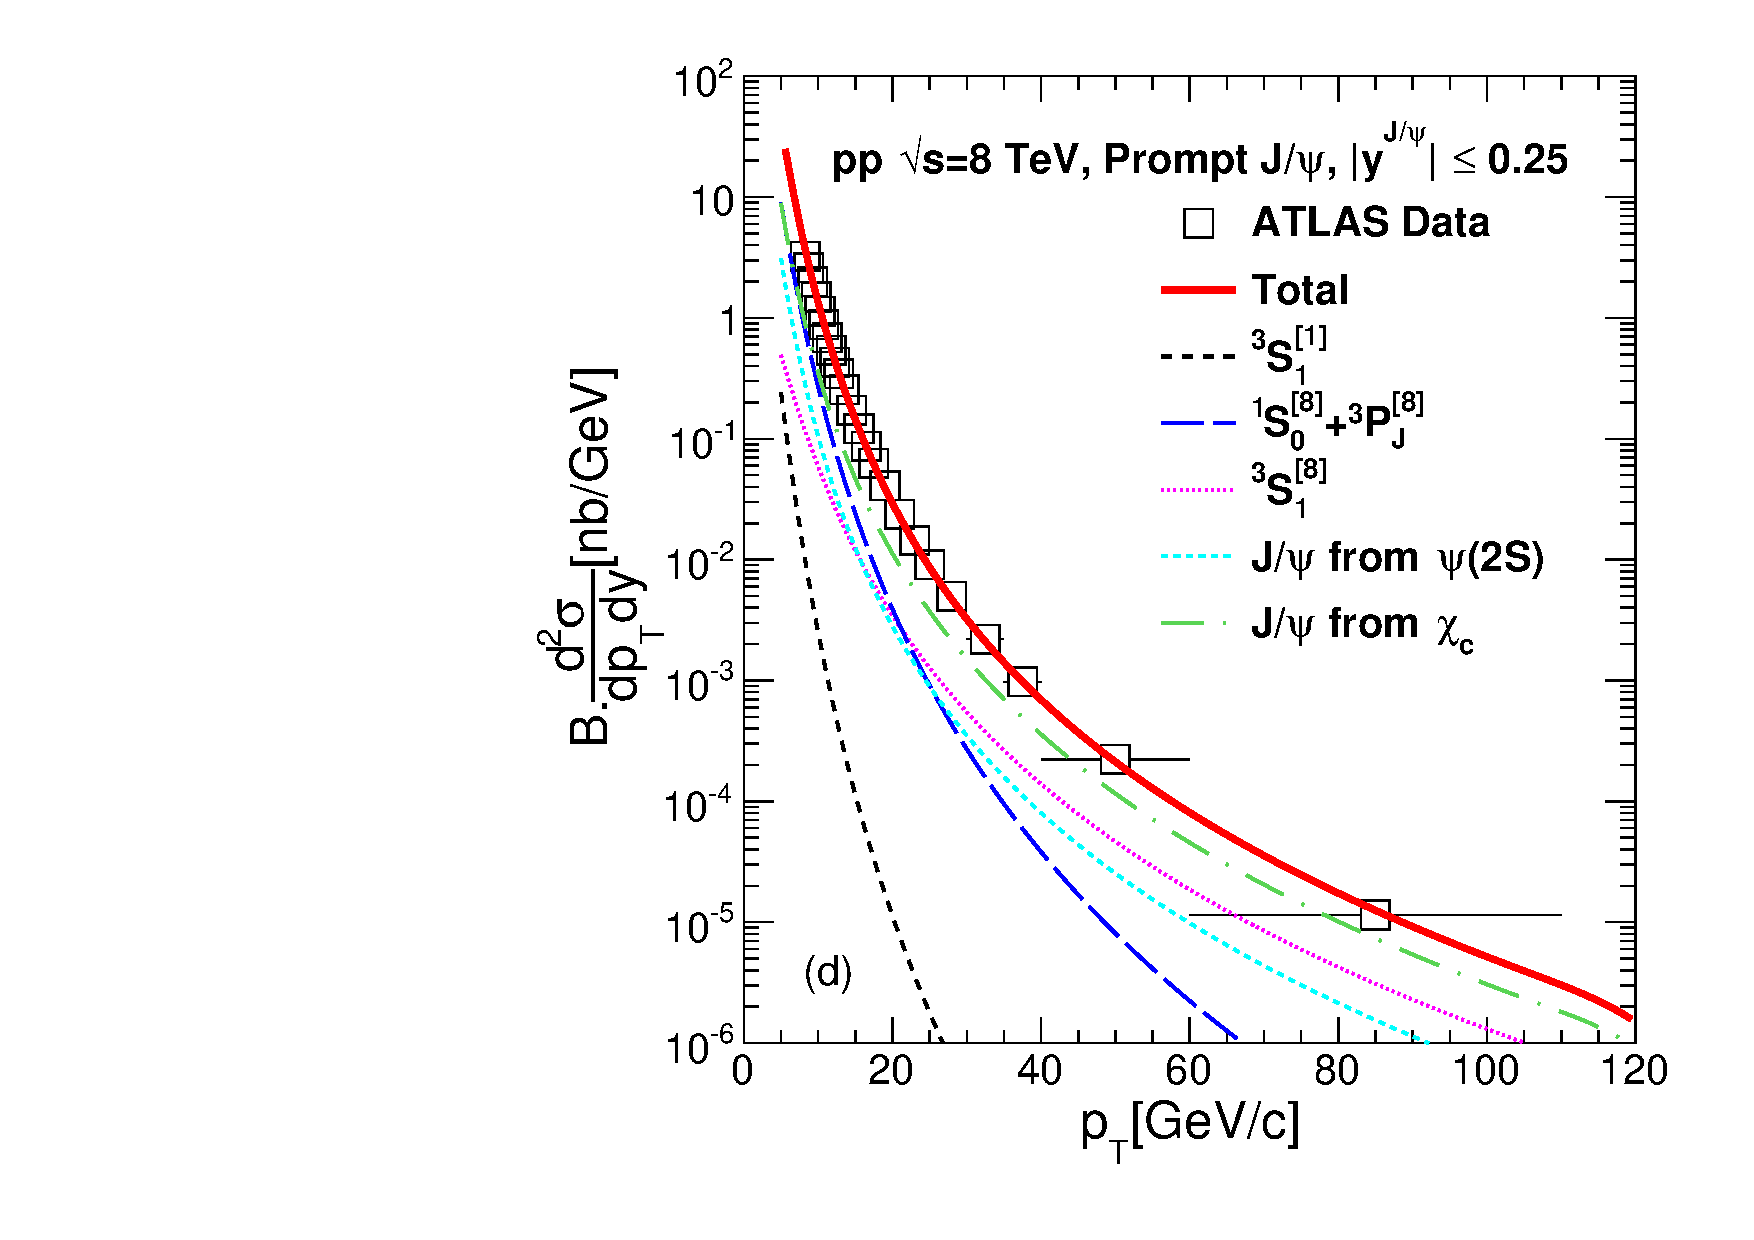
\includegraphics[width=0.49\textwidth]{ATLAS_8TeV_D2NDPtDy_PromptJPsi_Y0025_Pt.pdf}
\caption{(Color online) The NRQCD calculations of production cross section of $J/\psi$ in p+p collisions 
  as a function of transverse momentum compared with the measured data at LHC 
  (a) CMS data at $\sqrt{s}$ = 7 TeV~\cite{Chatrchyan:2011kc} 
  (b) CMS data at $\sqrt{s}$ = 7 TeV~\cite{Khachatryan:2015rra} 
  (c) ATLAS data at $\sqrt{s}$ = 7 TeV and
  (d) ATLAS data at $\sqrt{s}$ = 8 TeV~\cite{Aad:2015duc}. 
  The LDMEs are obtained by a combined fit of the LHC and Tevatron data.
}
\label{Fig:LDMEJPsi}
\end{figure}

\begin{figure}
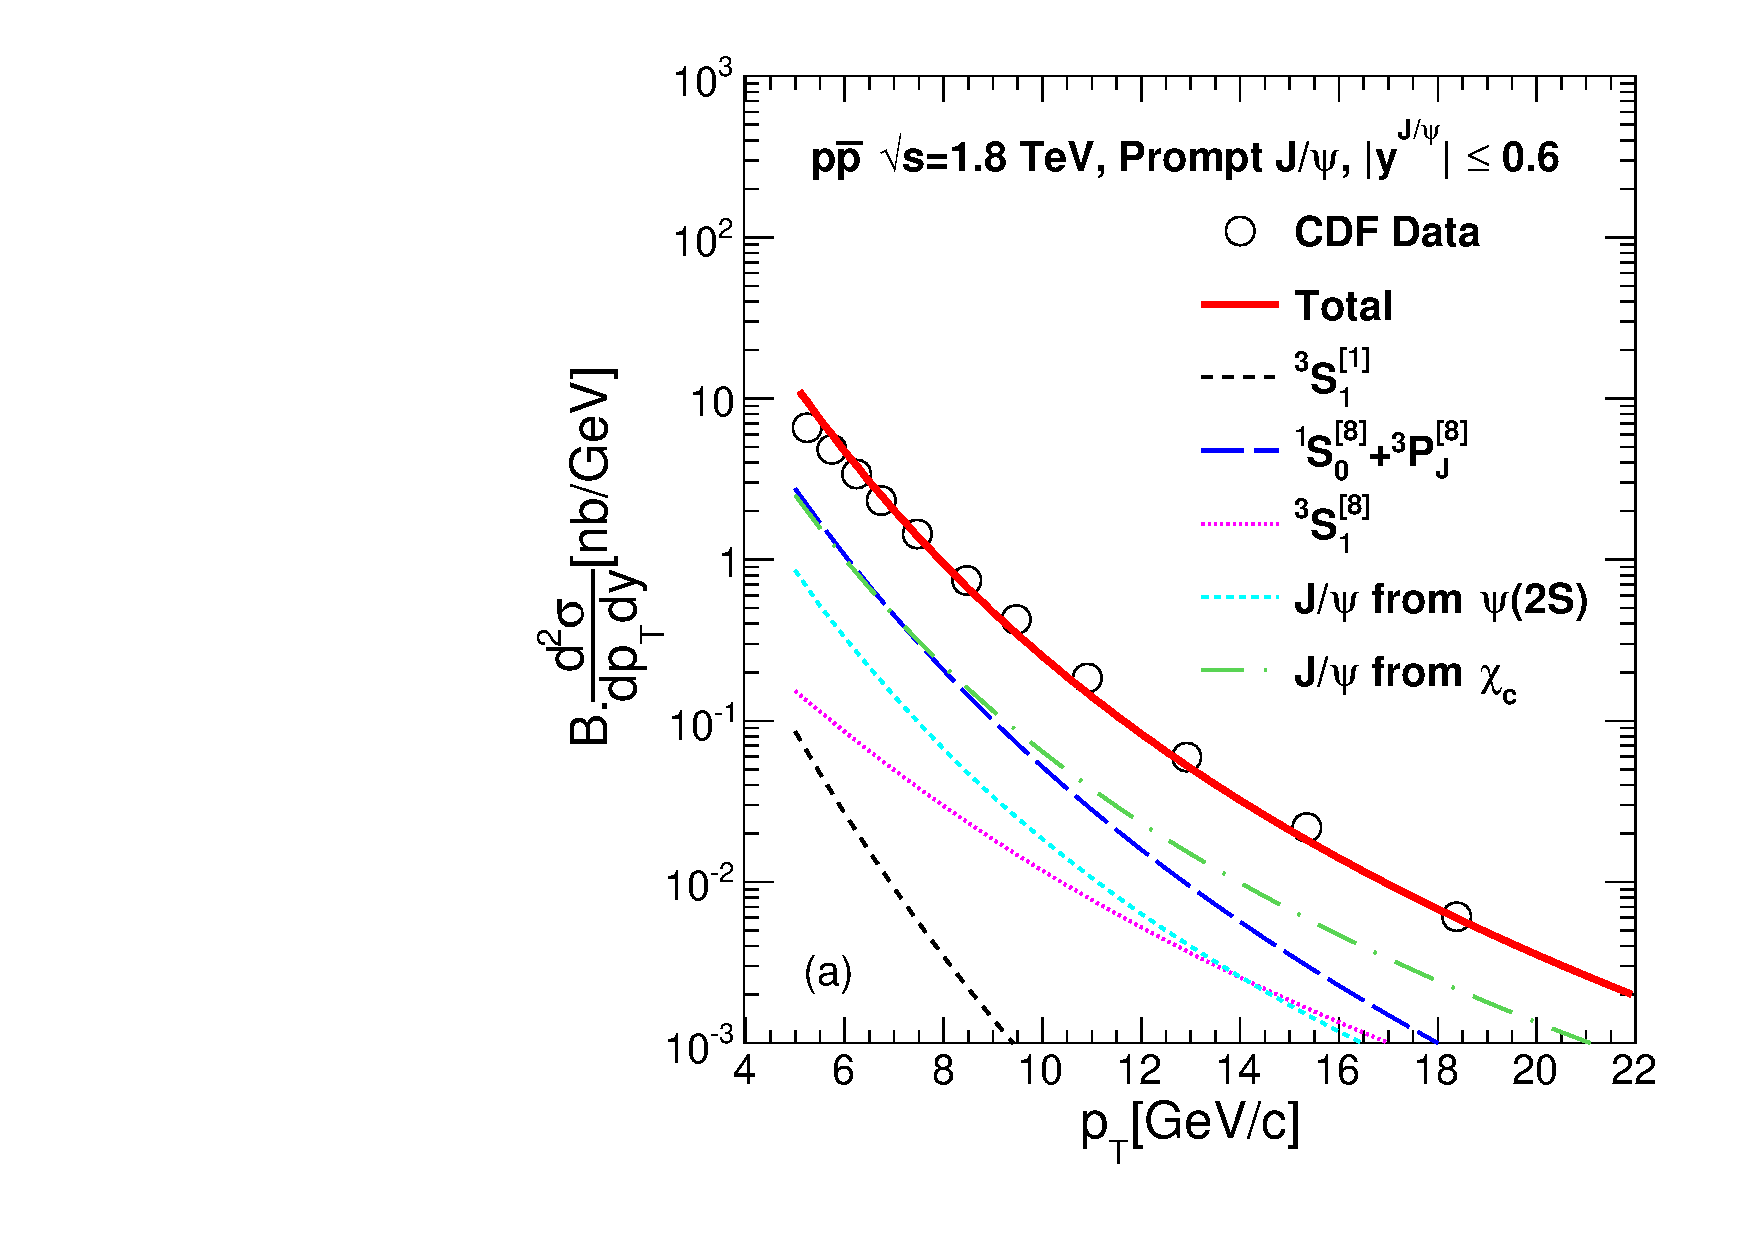
\includegraphics[width=0.49\textwidth]{CDF_RootS180TeV_D2NDPtDy_PromptJPsi_Y0006_Pt.pdf}
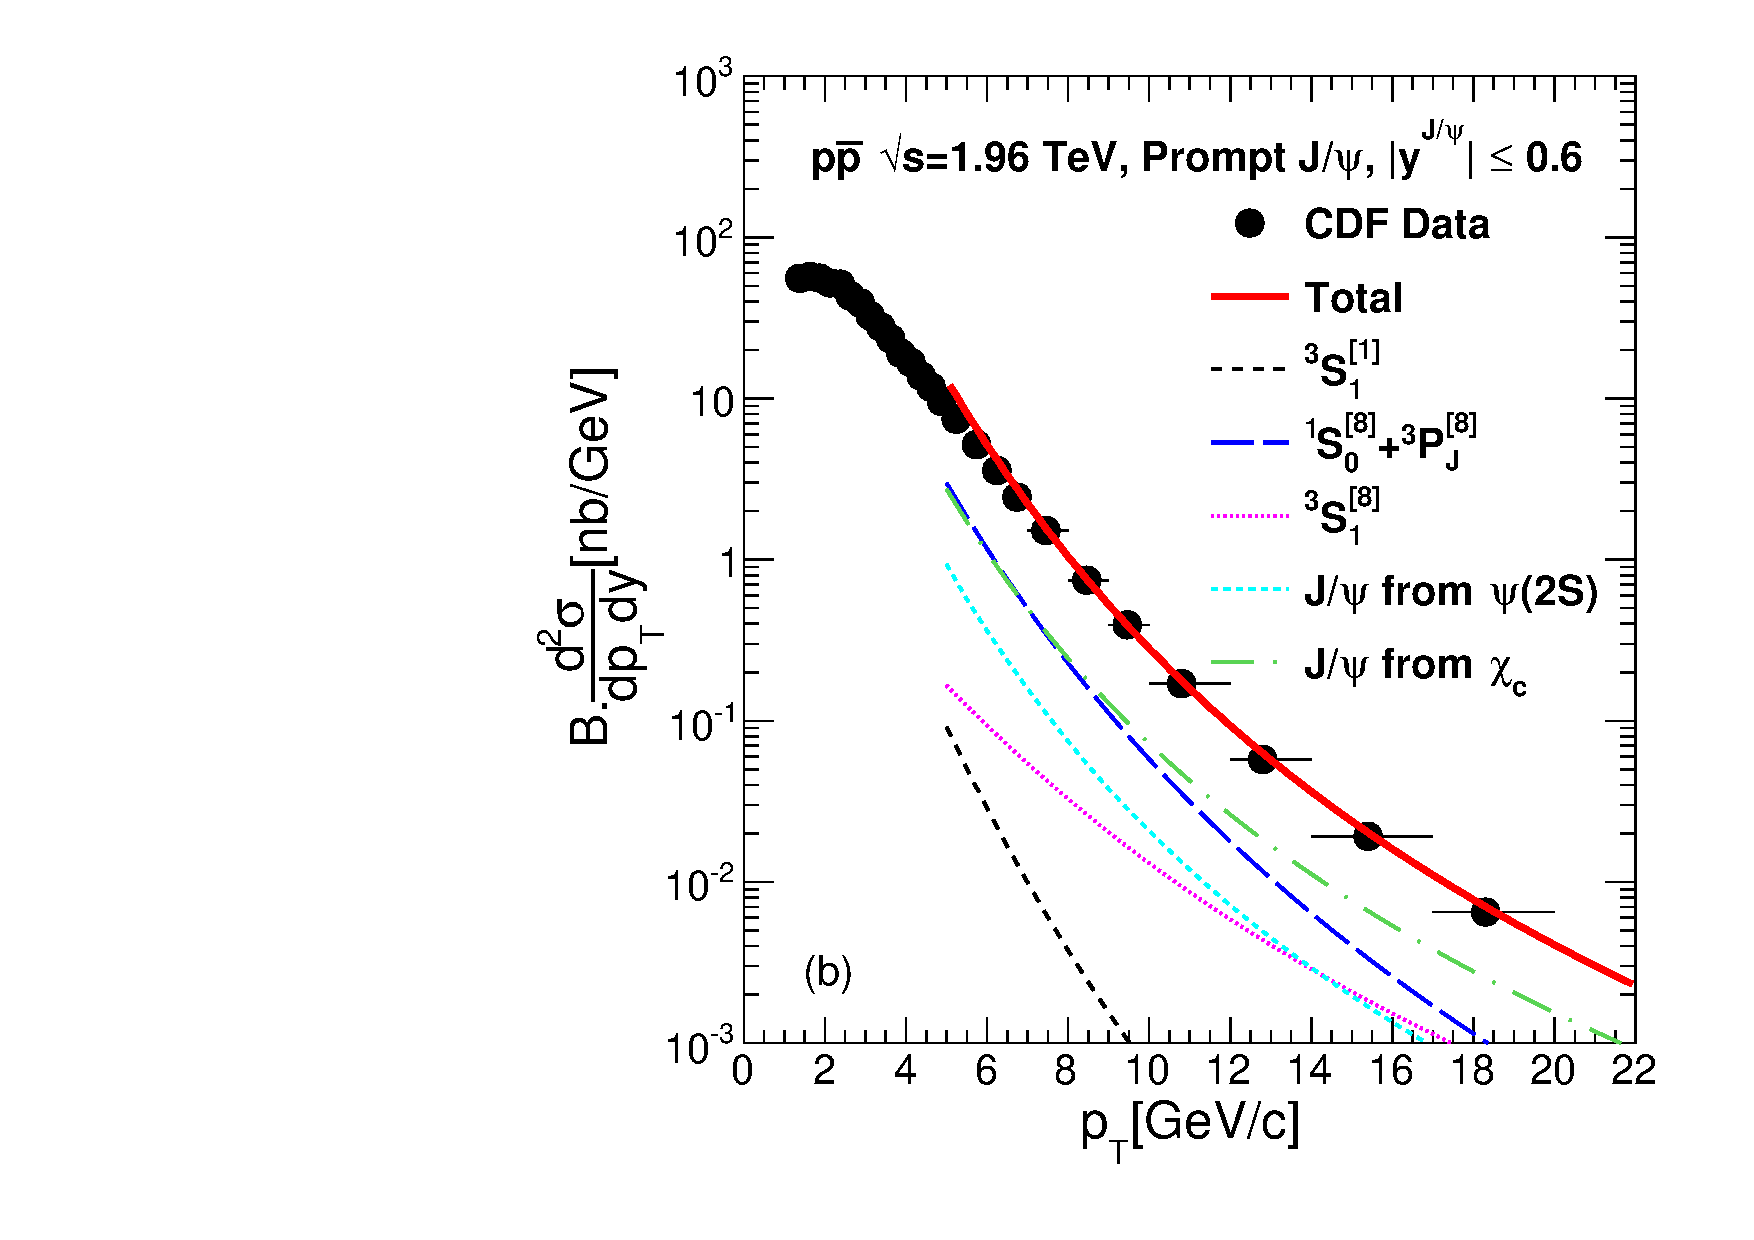
\includegraphics[width=0.49\textwidth]{CDF_196TeV_D2NDPtDy_PromptJPsi_Y0006_Pt.pdf}
\caption{(Color online) 
  The NRQCD calculations of production cross section of $J/\psi$ in p+${\bar {\rm p}}$ collisions 
  as a function of transverse momentum compared with the measured data at Tevatron 
  (a) CDF data at $\sqrt{s}$ = 1.8 TeV~\cite{Abe:1997jz} and
  (b) CDF data at $\sqrt{s}$ = 1.96 TeV~\cite{Acosta:2004yw}. 
  The LDMEs are obtained by a combined fit of the LHC and Tevatron data.
}
\label{Fig:LDMEJPsiCDF}
\end{figure}

\begin{figure}
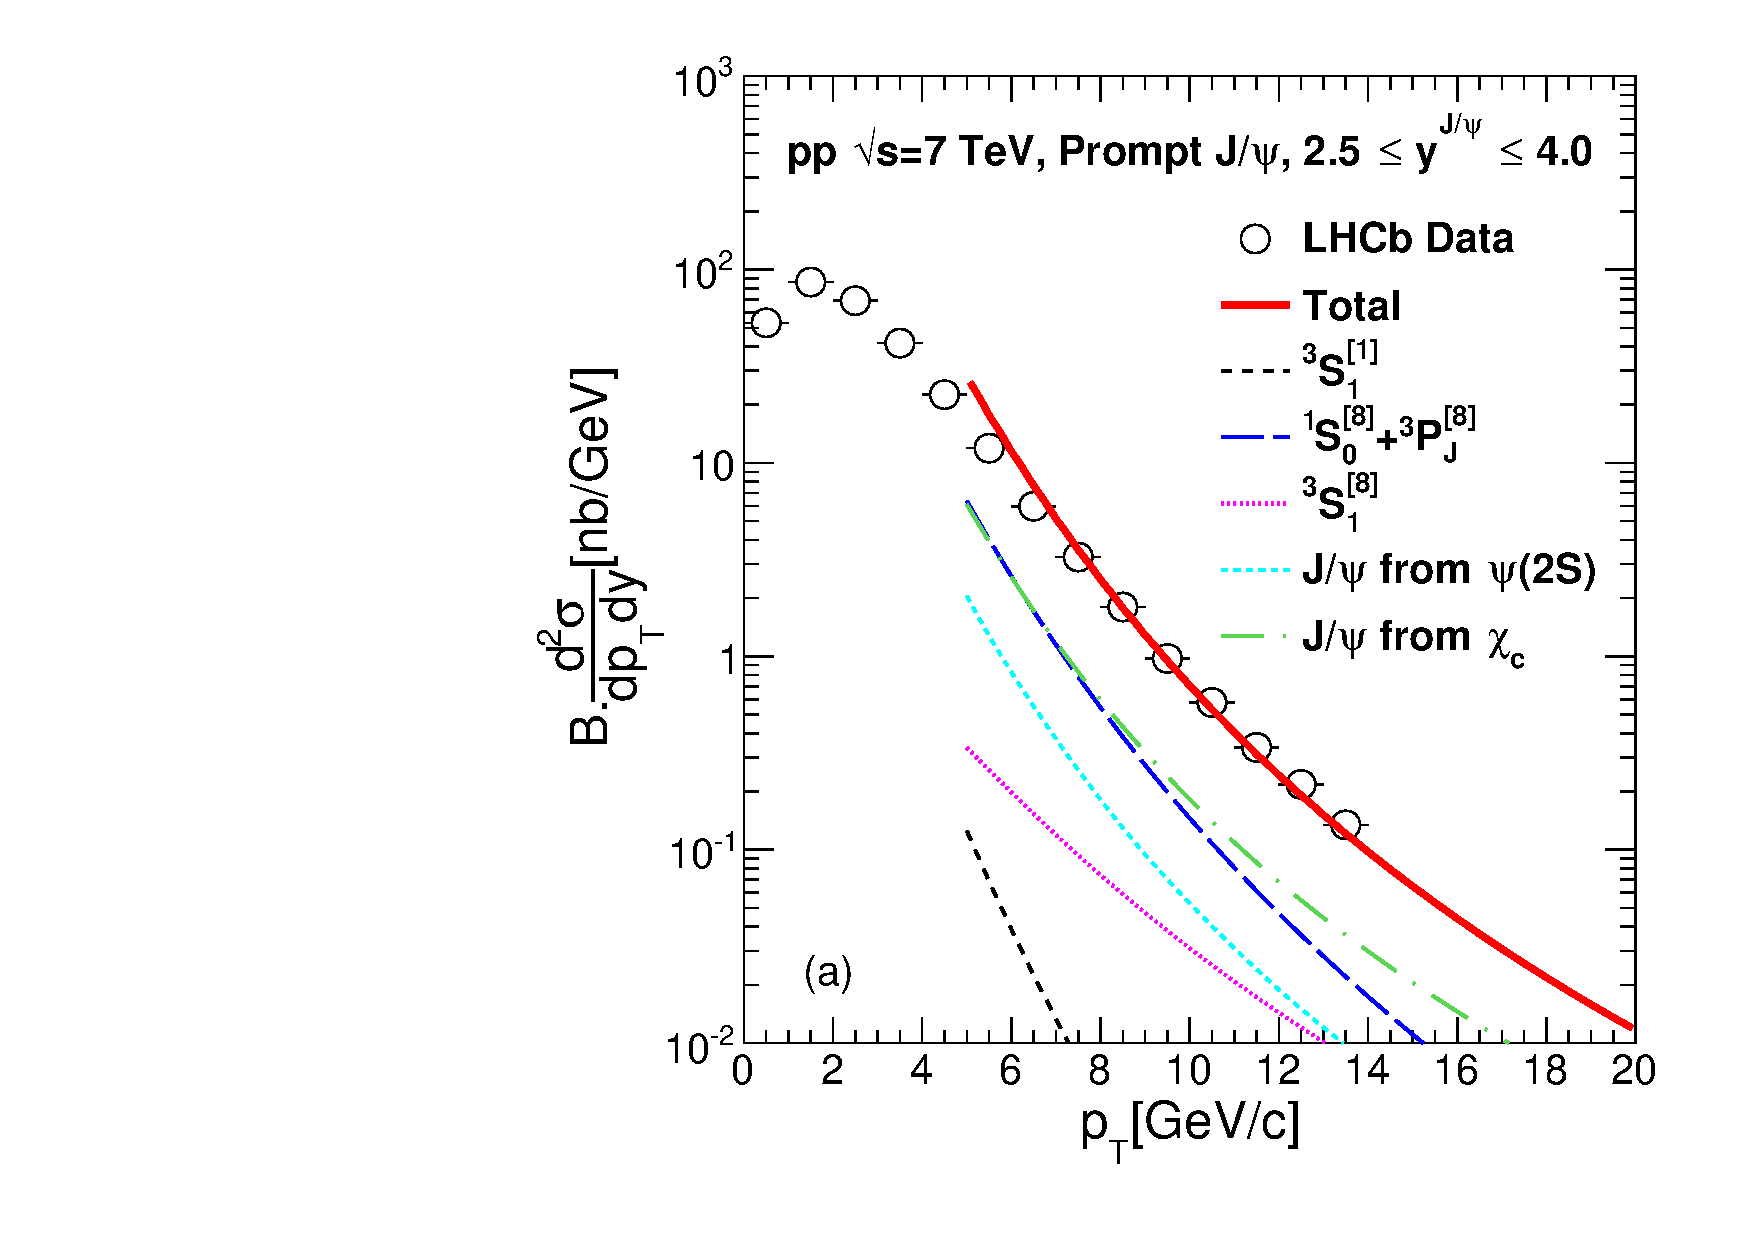
\includegraphics[width=0.49\textwidth]{LHCb_RootS7TeV_D2NDPtDy_PromptJPsi_Y2035_Pt.pdf}
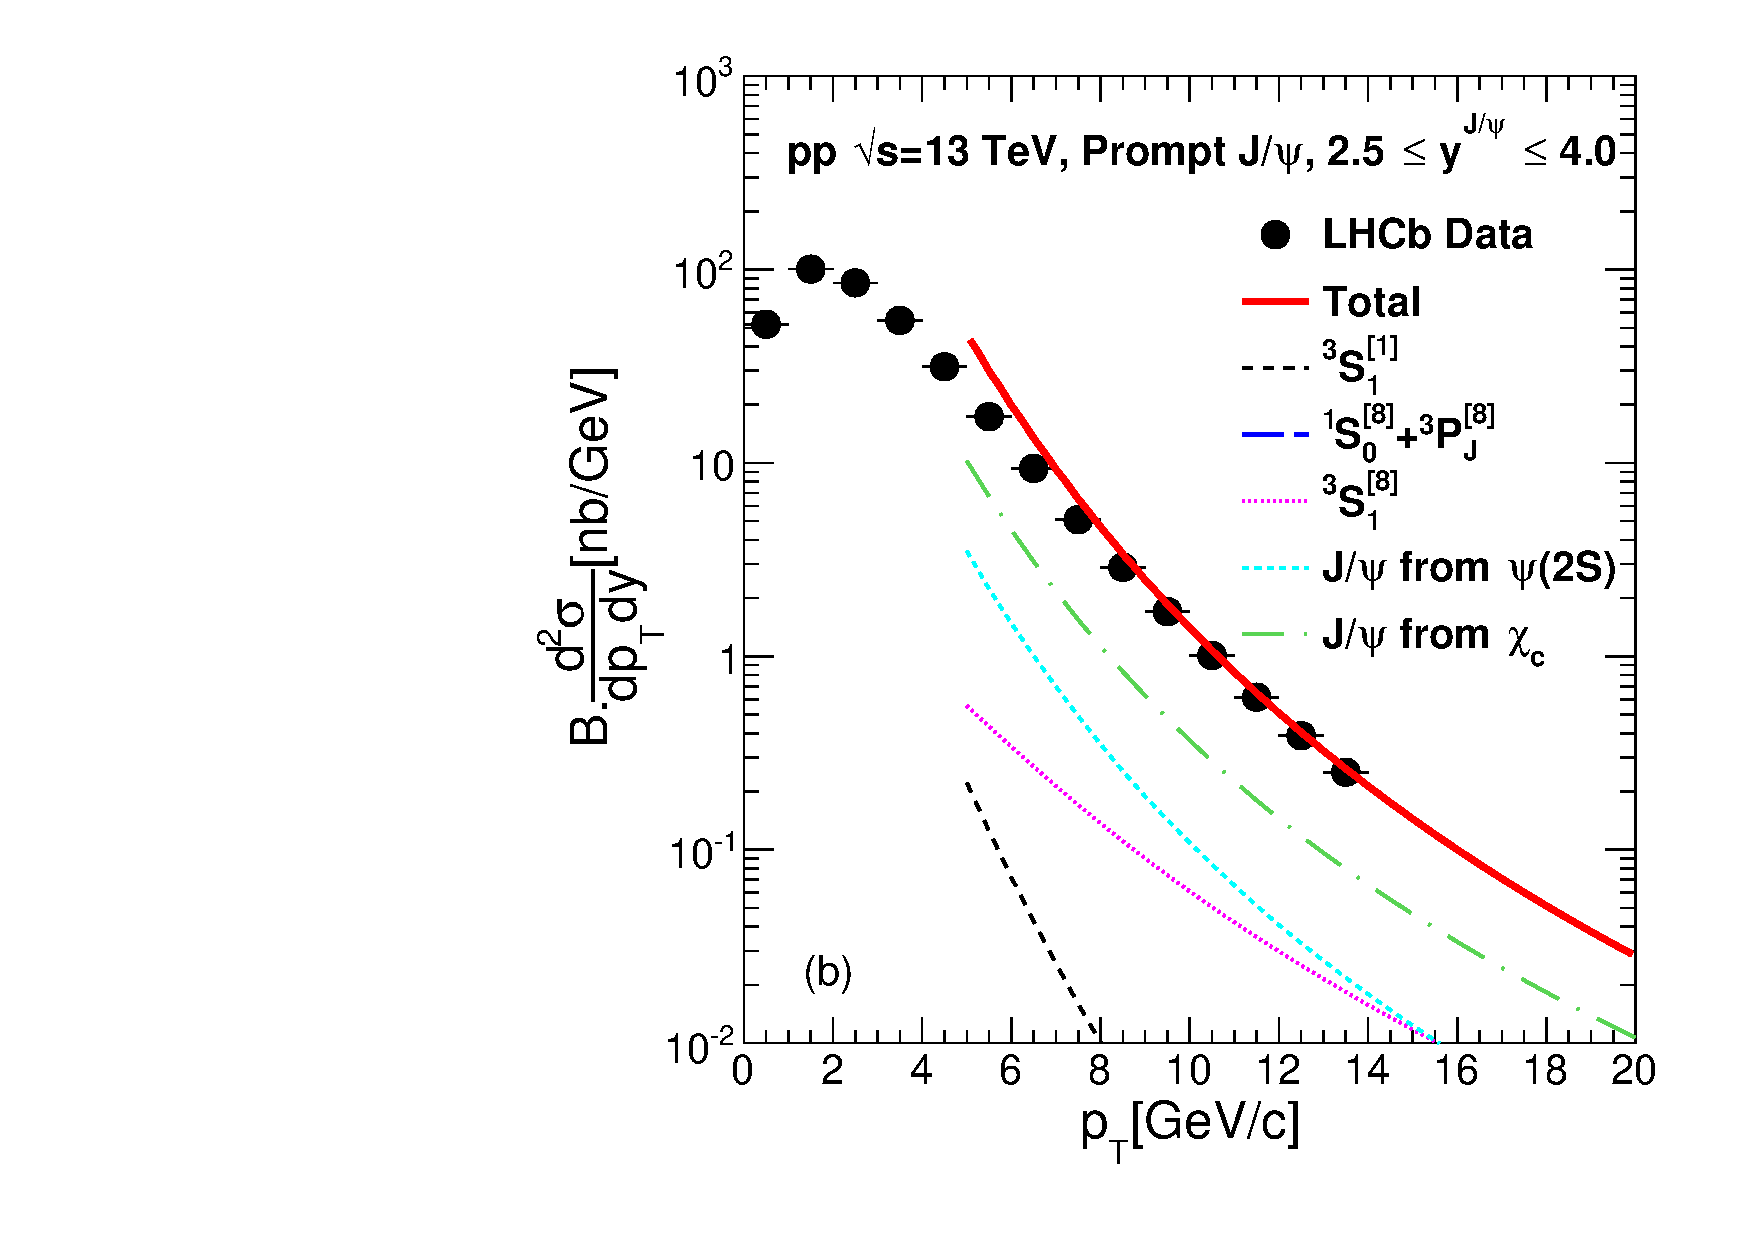
\includegraphics[width=0.49\textwidth]{LHCb_RootS13TeV_D2NDPtDy_PromptJPsi_Y2045_Pt.pdf}
\caption{(Color online) The NRQCD calculations of production cross section of $J/\psi$ in p+p collisions 
  as a function of transverse momentum compared with the measured data at LHC 
  (a) LHCb data at $\sqrt{s}$ = 7 TeV~\cite{Aaij:2011jh} and 
  (b) LHCb data at $\sqrt{s}$ = 13 TeV~\cite{Aaij:2015rla}. 
  The LDMEs are obtained by a combined fit of the LHC and Tevatron data.
}
\label{Fig:LDMEJPsiLHCb}
\end{figure}



%%%%%%%%%%%%%%%%%%%%%%%%%%%%%%%%%%%%%%%%%%%%%%%%%%%%%%%%%%%%%%%%%%%%%%%%%%%%%%%%






%%%%%%%%%%%%%%%%%%%%%%%%%%%%%%%%%%%%%%%%%%%%%%%%%%%%%%%%%%%%%%%%
\begin{figure}
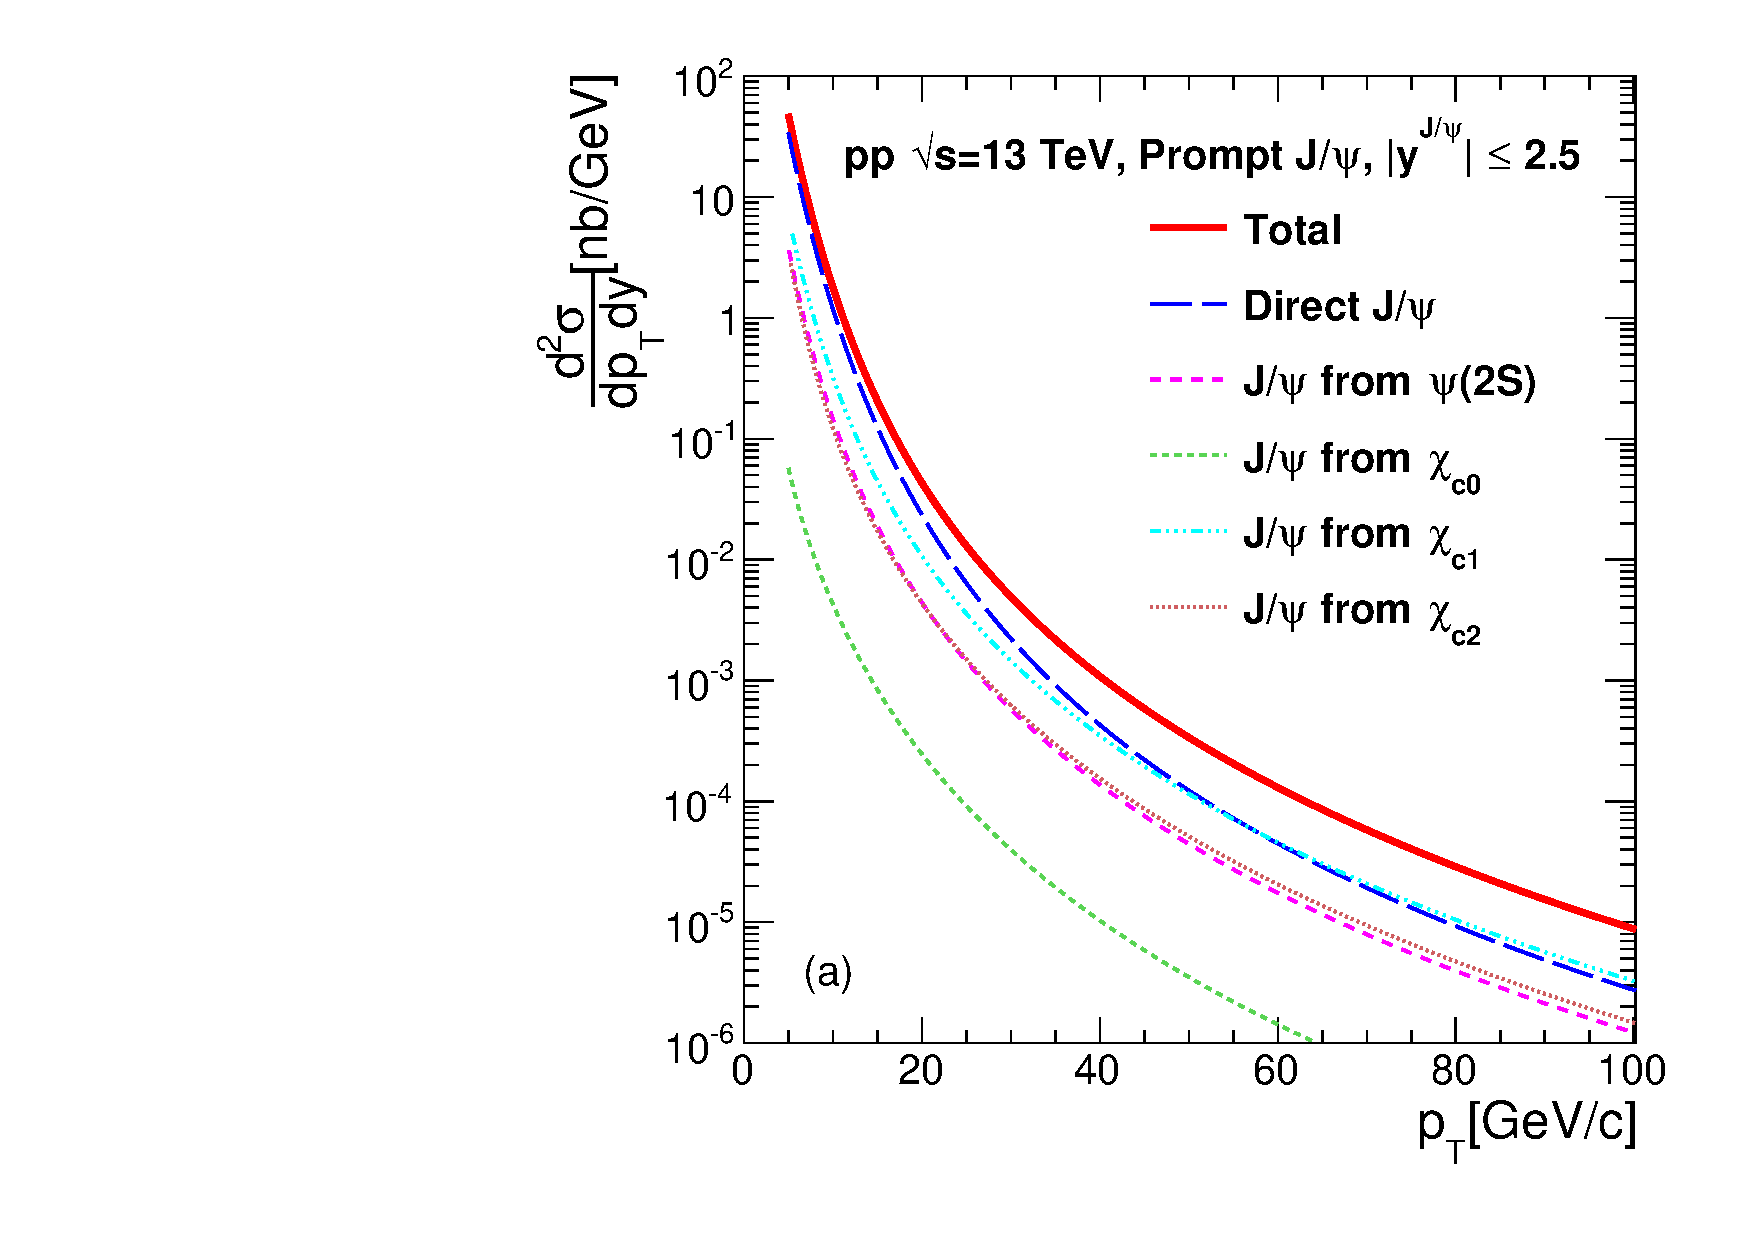
\includegraphics[width=0.49\textwidth]{Fig_ATLAS_D2NDPtDy_RootS13TeV_PromptJPsi_Y2525.pdf}
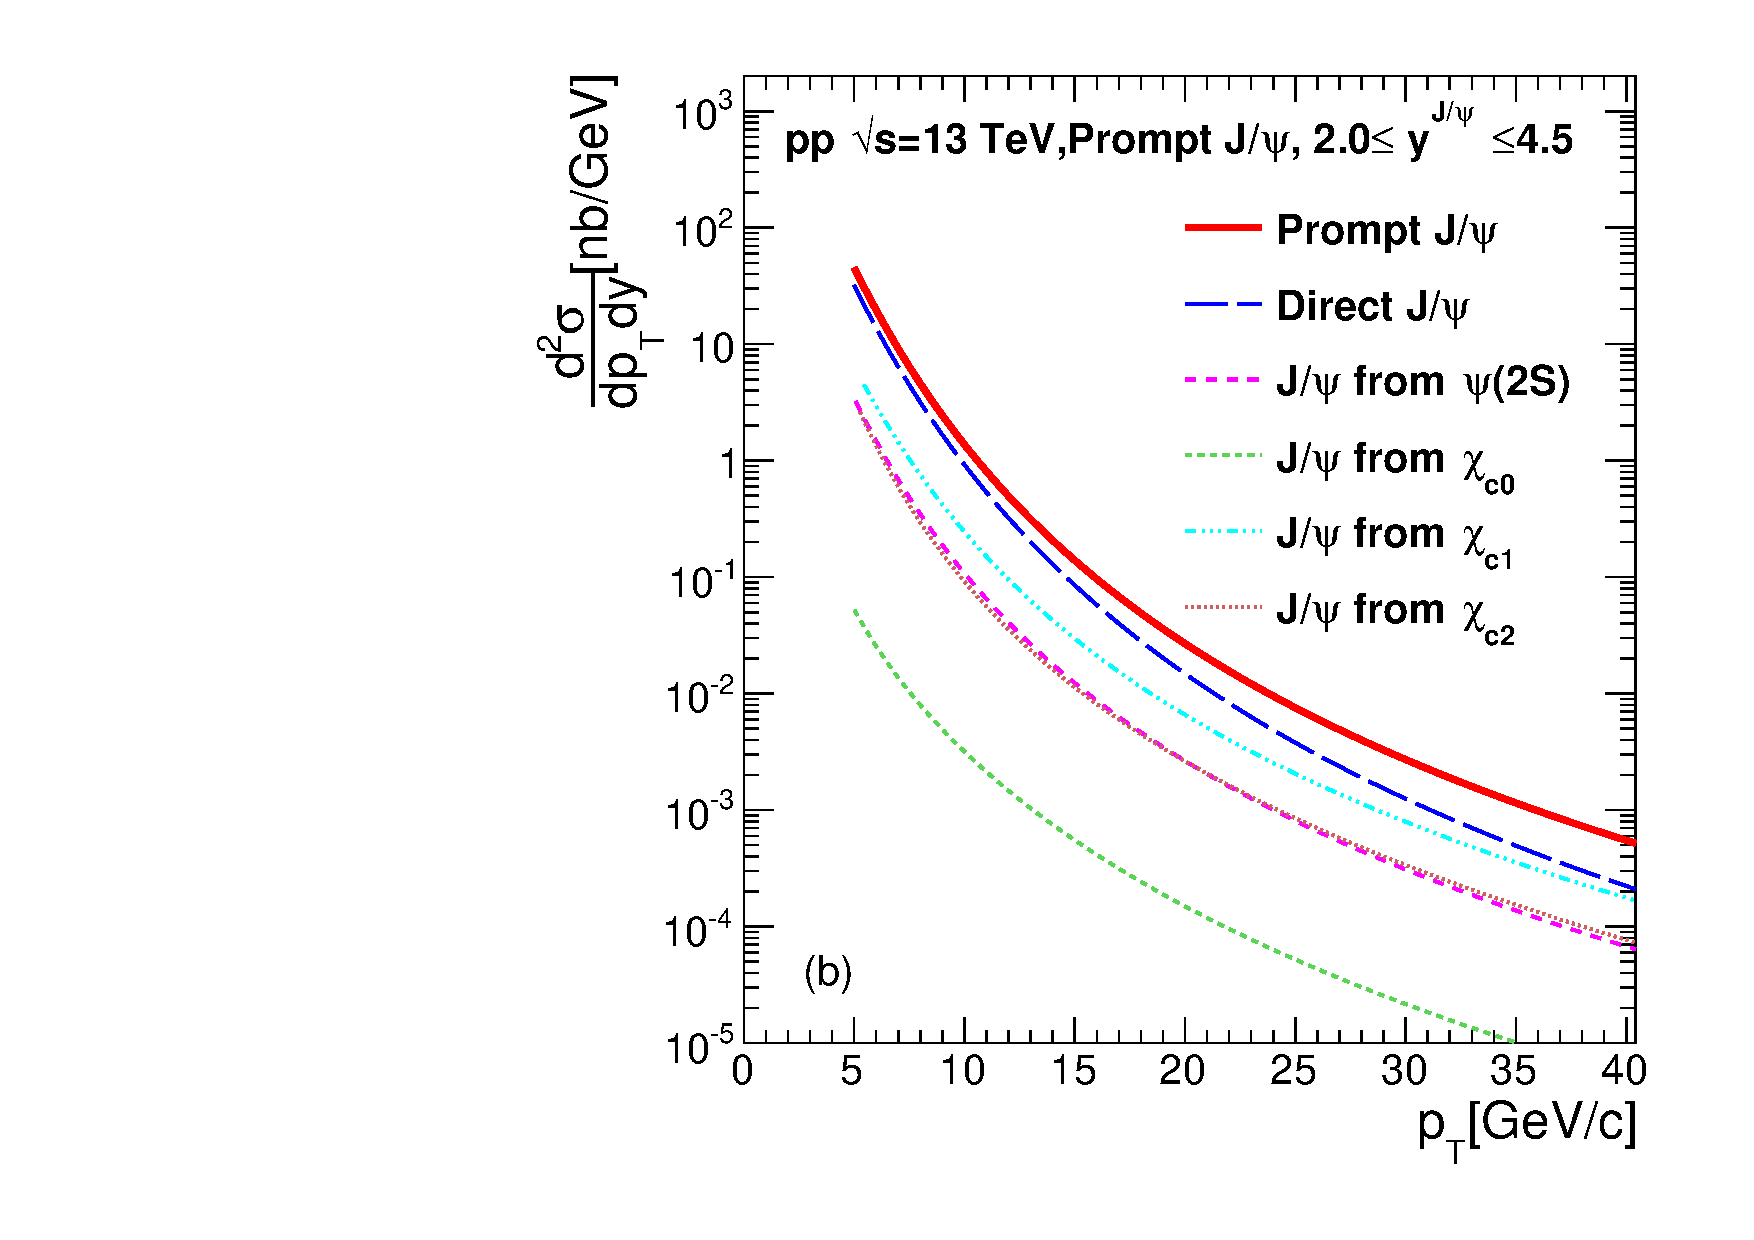
\includegraphics[width=0.49\textwidth]{Fig_ALICE_D2NDPtDy_RootS13TeV_PromptJPsi_Y2045.pdf}
\caption{(Color online) The NRQCD calculations of production cross section of $J/\psi$ in p+p collisions 
  as a function of transverse momentum at $\sqrt{s}$ = 13 TeV. The calculations are shown in the kinematic
  bins relevant to (a) CMS, ATLAS and (b) ALICE, LHCb detectors at LHC. For the J/$\psi$ meson all the 
  relevant contributions from higher mass states are also shown.
}
\label{Fig:SigmaJPsi}
\end{figure}


\begin{figure}
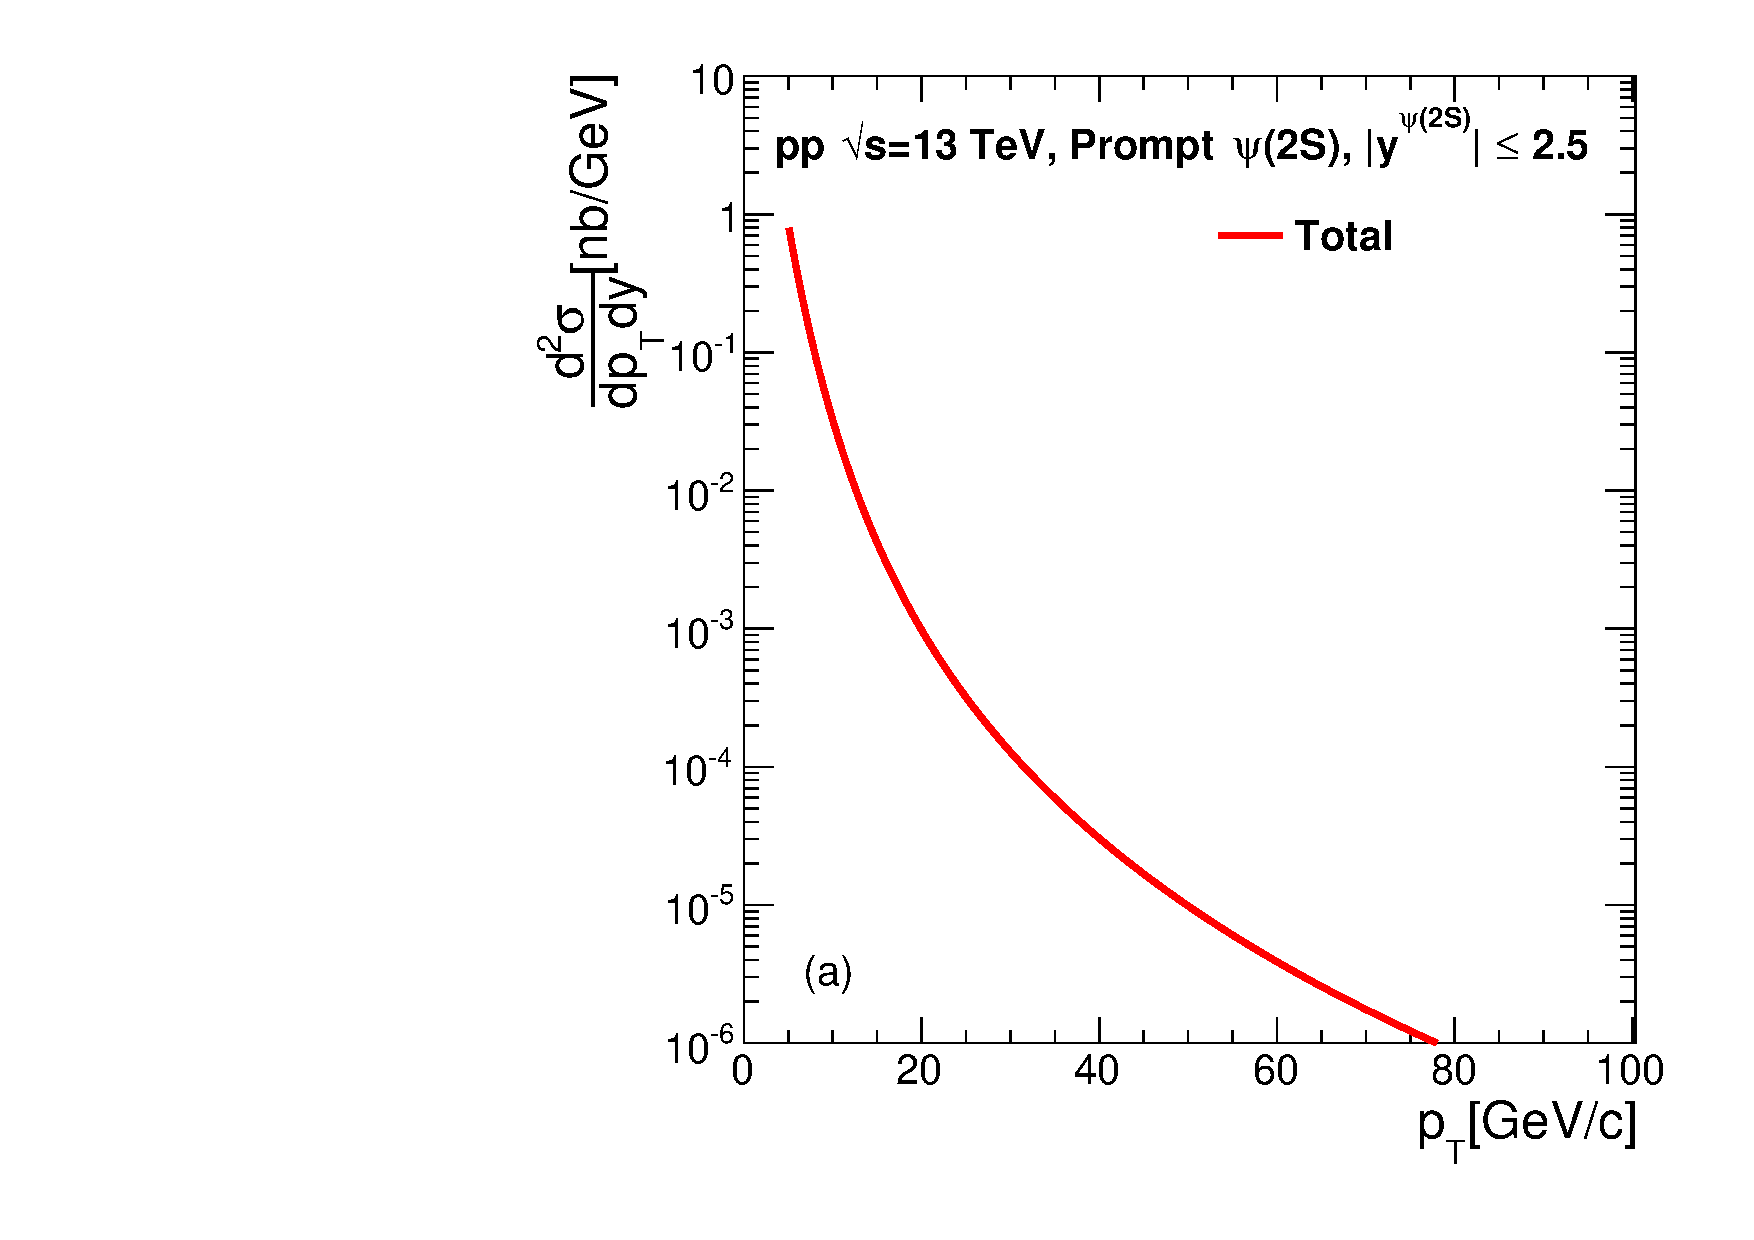
\includegraphics[width=0.49\textwidth]{Fig_ATLAS_D2NDPtDy_RootS13TeV_DirectPsi_Y2525.pdf}
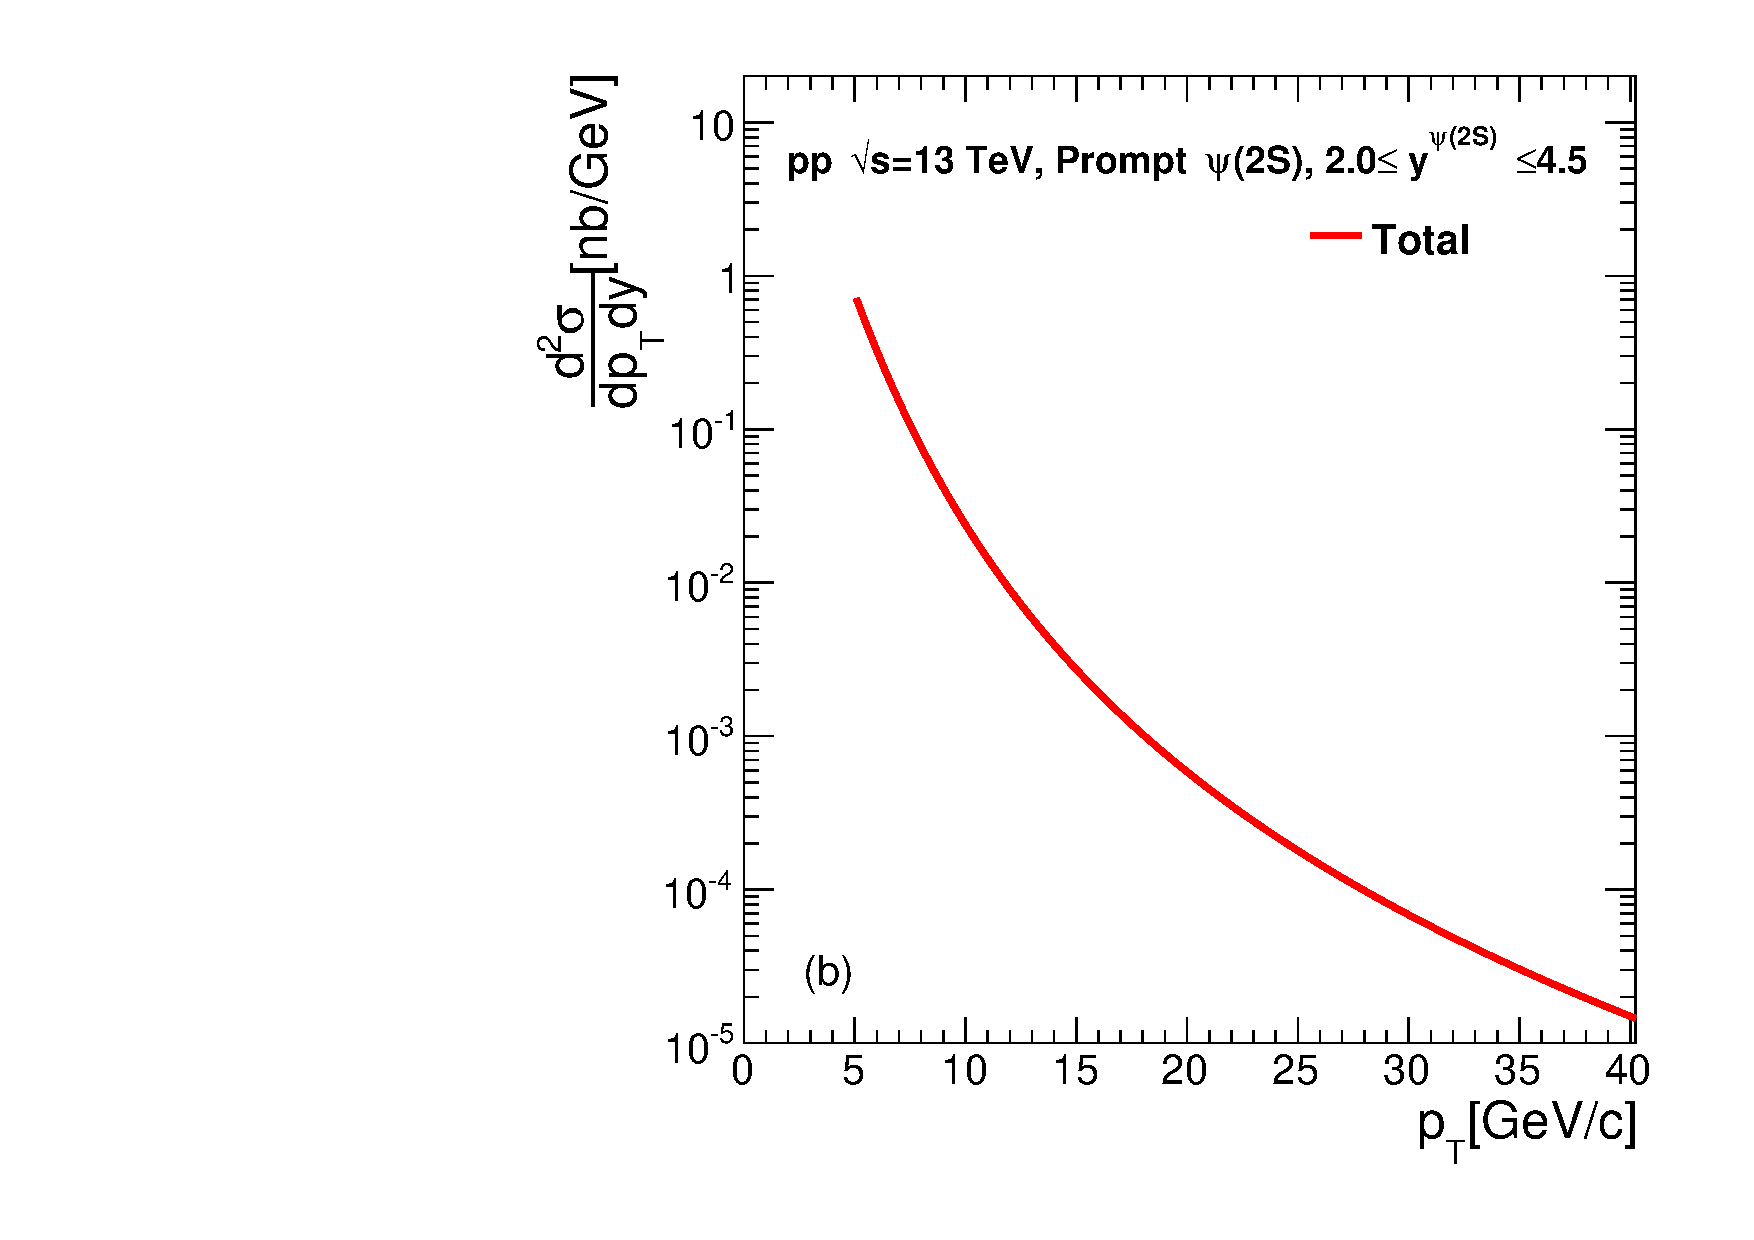
\includegraphics[width=0.49\textwidth]{Fig_ALICE_D2NDPtDy_RootS13TeV_DirectPsi_Y2045.pdf}
\caption{(Color online) The NRQCD calculations of production cross section of $\psi$(2S) in p+p collisions 
  as a function of transverse momentum at $\sqrt{s}$ = 13 TeV. The calculations are shown in the kinematic
  bins relevant to (a) CMS, ATLAS and (b) ALICE, LHCb detectors at LHC. 
}
\label{Fig:SigmaPsi}
\end{figure}


\begin{figure}
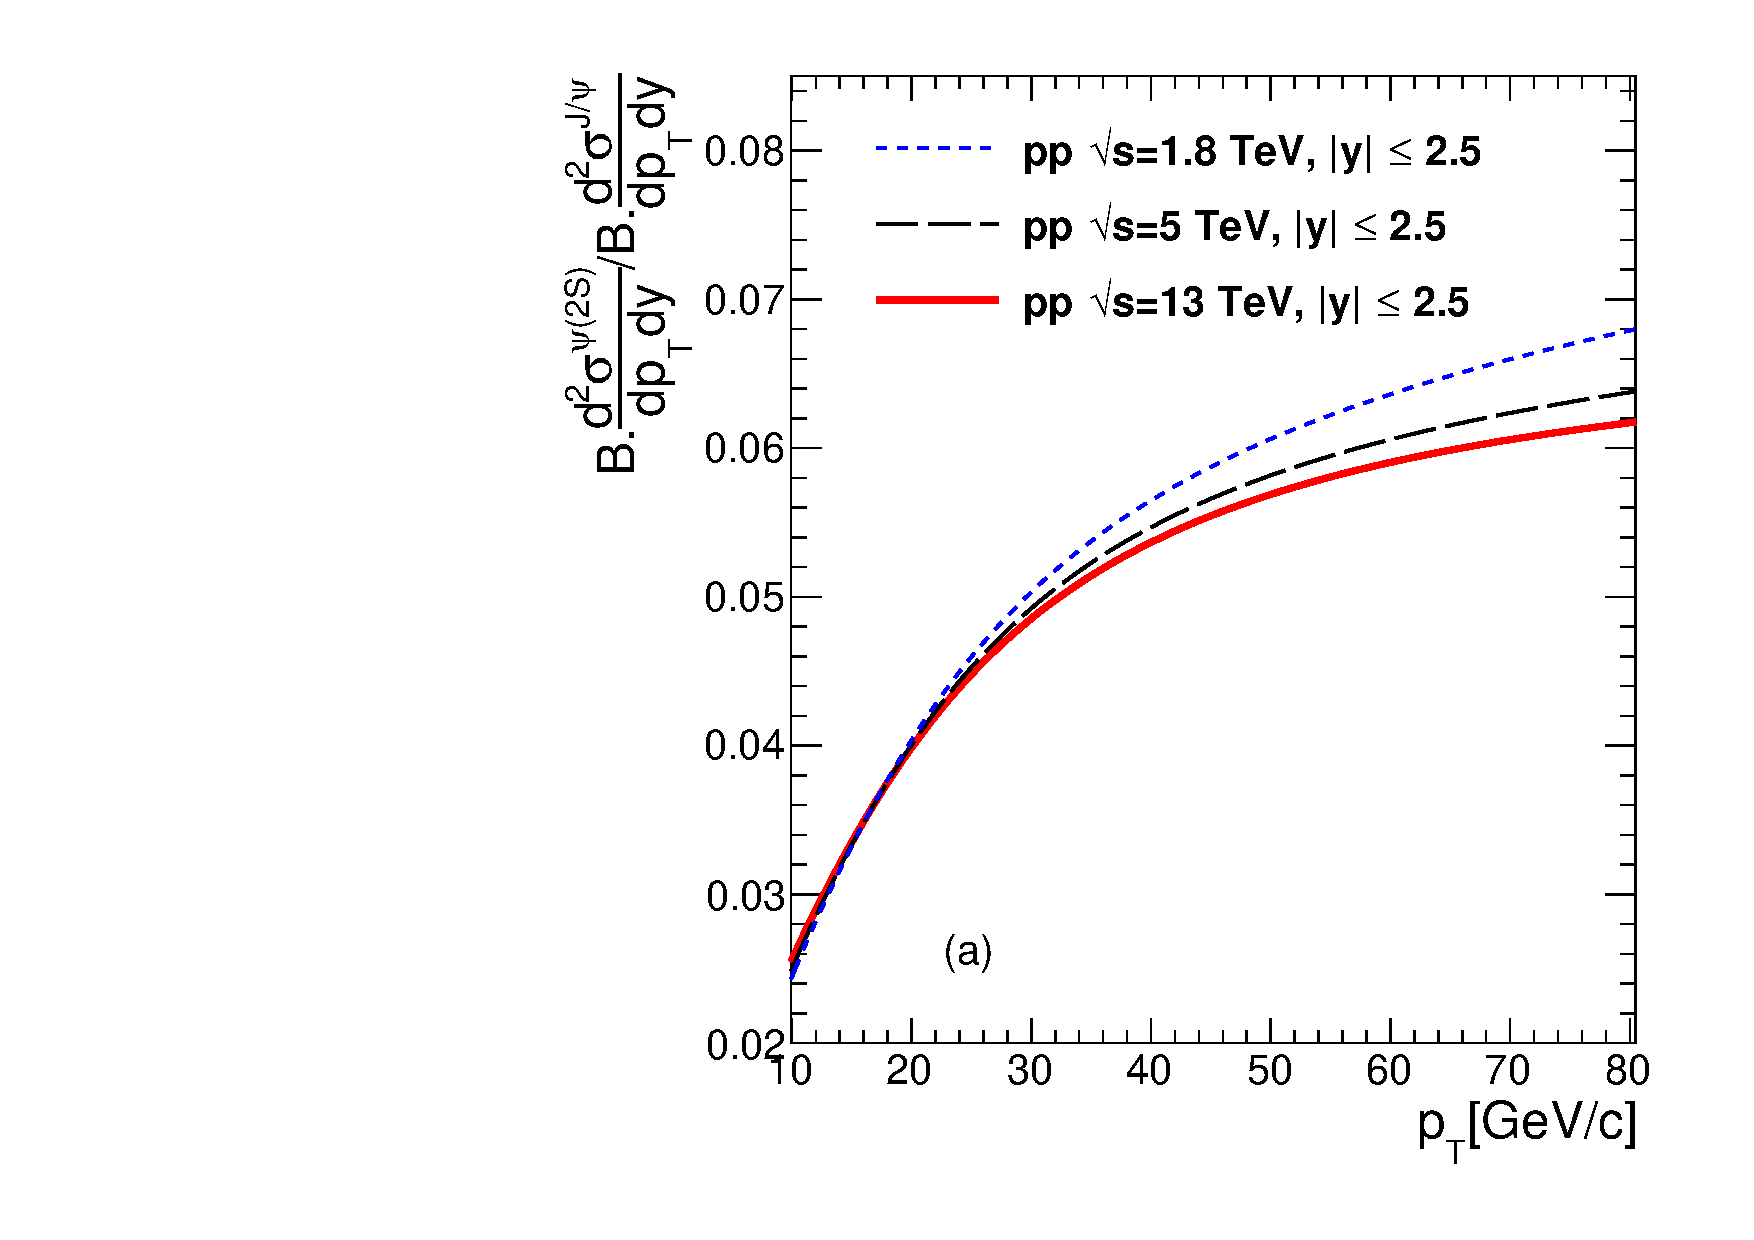
\includegraphics[width=0.49\textwidth]{Fig_ATLAS_D2NDPtDy_DirectPsi_DirectJPsi_Y2525.pdf}
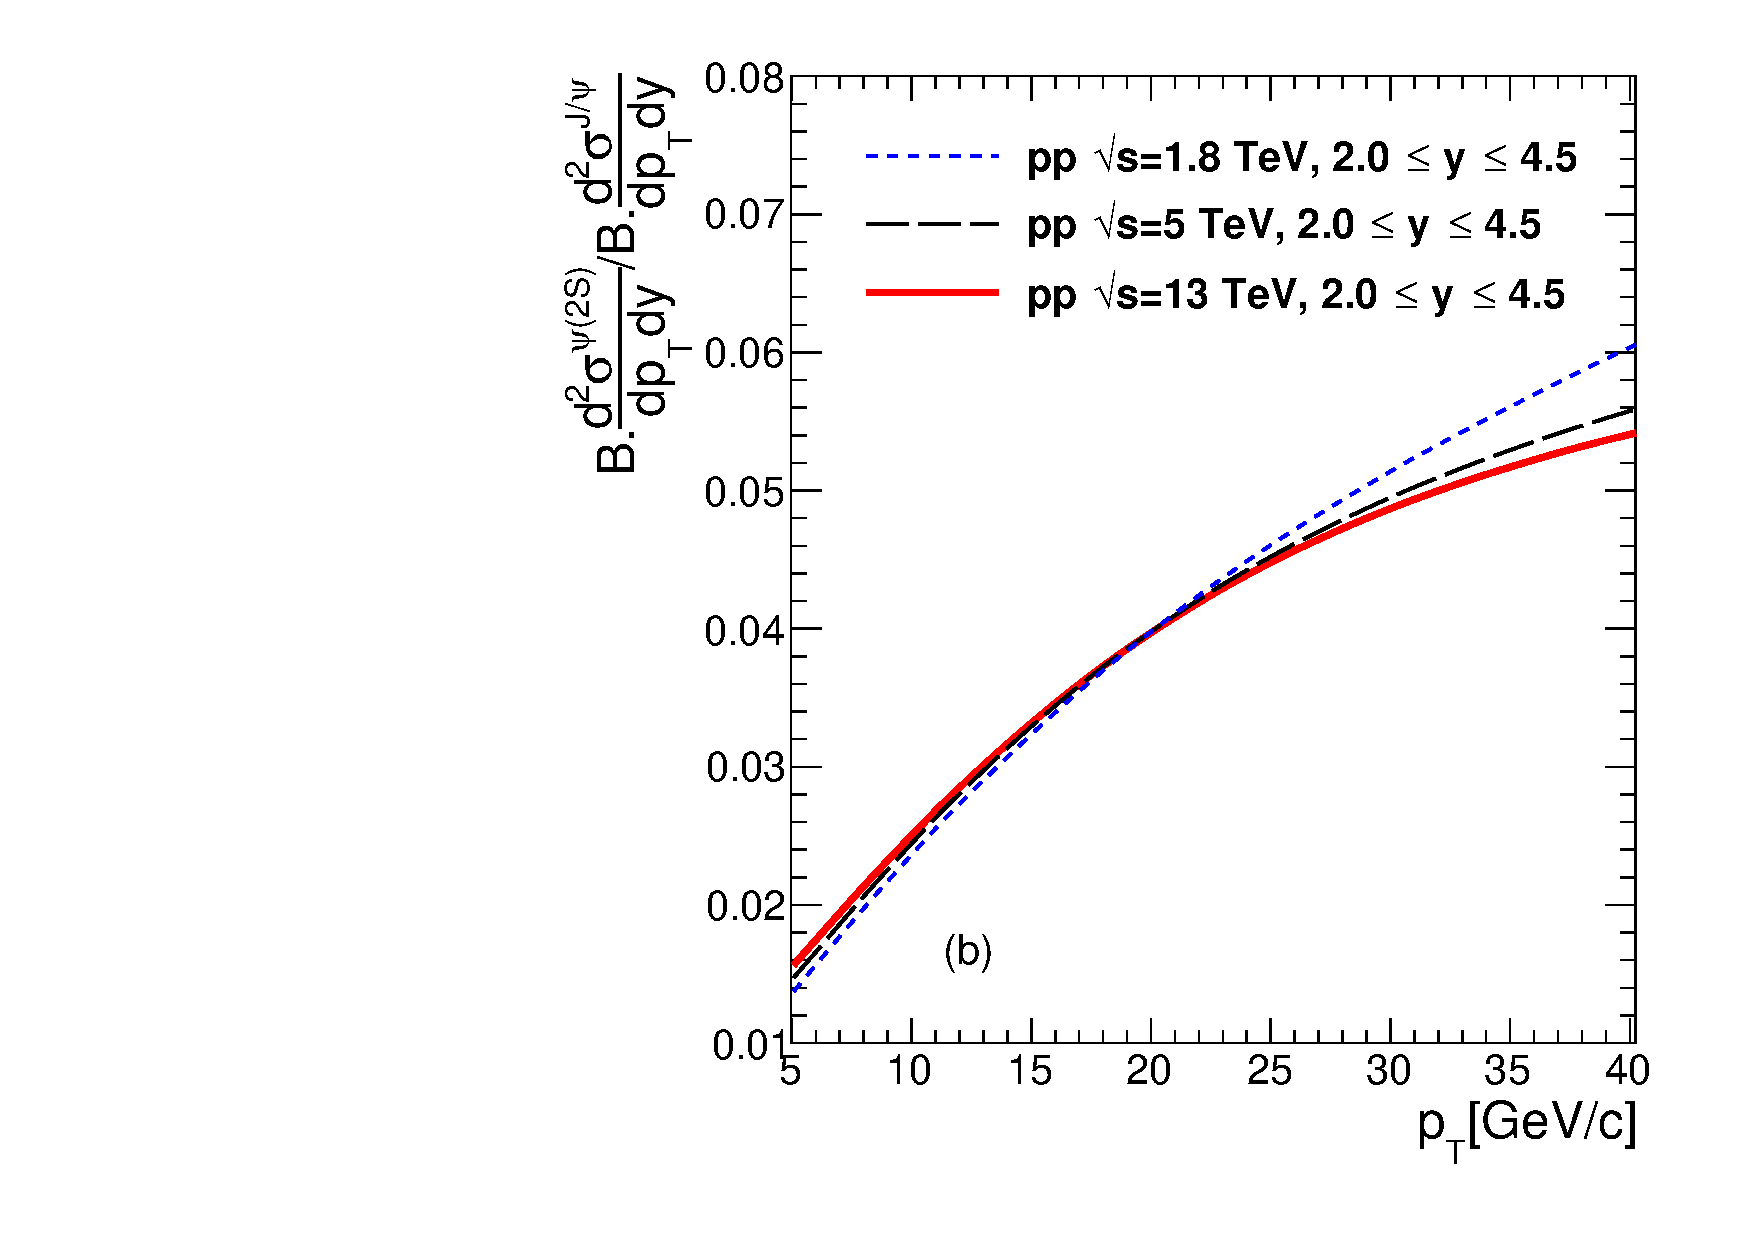
\includegraphics[width=0.49\textwidth]{Fig_ALICE_2045_RootS5TeV_Psi_JPsi_Pt.pdf}
\caption{(Color online) The NRQCD calculations of production cross section ratios of $\psi$(2S) and $J/\psi$
  in p+p collisions as a function of transverse momentum at $\sqrt{s}$ = 1.8, 5 and 13 TeV. 
The calculations are shown in  the kinematic bins relevant for (a) CMS, ATLAS and (b) ALICE, LHCb 
detectors at LHC. 
}
\label{Fig:RatioSigma_13TeV}
\end{figure}






%%%%%%%%%%%%%%%%%%%%%%%%%%%%%%%%%%%%%%%%%%%%%%%%%%%%%%%%%%%%%%%%%%%%%%%%%%%%%%%%%%%%%%%

\section{Results and Discussions}
   As discussed in the last section there are two free parameters for $J/\psi$, 
two for $\psi$(2S) and one for $\chi_{cJ}$ to be obtained from the experiments. 
CDF~\cite{Abe:1997yz} has measured the feed-down contribution from the
$\chi_{cJ}$ states to $J/\psi$, we use this data to obtain $\chi_{cJ}$
color octet LDME. Figure~\ref{Fig:LDMEChicCDF} shows NRQCD calculations 
of production cross section of  $J/\psi$ from $\chi_{c1}$ and $\chi_{c2}$ 
decays in p+{$\bar {\rm p}$} collisions at $\sqrt{s}$ = 1.8 TeV as a function 
of the $J/\psi$ transverse momentum. The calculations are compared 
with the data measured by CDF experiment at Tevatron~\cite{Abe:1997yz}. 
The $\chi_{c}$ color octet LDMEs are obtained by fitting this data and 
its value is 
\begin{equation}
\begin{split}
M_{L}(Q\barQ([^3S_1]_{8})\rightarrow \chi_{c0})/m_{\charm}^2 & 
     = (0.00157\pm {\color{black} 0.00159})\,{\rm GeV^3}\;,
\label{eq:Mchicn1CO_val}
\end{split}
\end{equation}
with a $\chi^2/dof=1.86$. 
 The measured yields of prompt $\psi(2S)$ from the following datasets
are used to obtain color-octet matrix elements for $\psi(2S)$ 
\begin{enumerate}
\item{CMS results at $\sqrt{S}=7$~TeV~\cite{Chatrchyan:2011kc,Khachatryan:2015rra}}.
\item{ATLAS results at $\sqrt{S}=7$ and 8 ~TeV~\cite{Aad:2015duc}}.
\item{CDF results at $\sqrt{S}=1.8$~TeV~\cite{Abe:1997jz}}.
\item{CDF results at $\sqrt{S}=1.96$~TeV~\cite{Acosta:2004yw}}.
\item{LHCb results at $\sqrt{S}=7$~TeV~\cite{Aaij:2012ag}}.
\end{enumerate}
Figure~\ref{Fig:LDMEPsi2S} shows the NRQCD calculations of production cross section of 
$\psi$(2S) in p+p collisions as a function of transverse momentum compared with the 
measured data at LHC in panels
(a) CMS data at $\sqrt{s}$ = 7 TeV~\cite{Chatrchyan:2011kc},
(b) CMS data at $\sqrt{s}$ = 7 TeV~\cite{Khachatryan:2015rra}, 
(c) ATLAS data at $\sqrt{s}$ = 7 TeV and, 
(d) ATLAS data at $\sqrt{s}$ = 8 TeV~\cite{Aad:2015duc}. 
%The LDMEs are obtained by a combined fit of this LHC data along with Tevatron data
%shown in Fig~\ref{Fig:LDMEPsi2SCDF}.
 Figure~\ref{Fig:LDMEPsi2SCDF} shows the NRQCD calculations of production cross section 
of $\psi$(2S) in p+{$\bar {\rm p}$} collisions as a function of transverse momentum compared 
with the measured data at Tevatron in panels (a) CDF data at $\sqrt{s}$ = 1.8 TeV~\cite{Abe:1997jz} 
and (b) CDF data at $\sqrt{s}$ = 1.96 TeV~\cite{Acosta:2004yw}. 
%The LDMEs are obtained by a combined fit of the Tevatron and LHC data
We obtain following values of $\psi(2S)$ color-octet matrix elements by a combined fit of 
the Tevatron and LHC data   
\begin{equation}
  \begin{split}
    M_{L}(c\barc([^3S_1]_{8})\rightarrow \psi(2S)) &= (0.00190\pm 0.00002 \pm 0.00001) \, {\rm GeV^3}\\
    M_{L}(c\barc([^1S_0]_{8})\rightarrow \psi(2S)) &= (0.0264\pm 0.0003 \pm 0.0004) \,{\rm GeV^3}\\
    &= M_{L}(c\barc([^3P_0]_{8})\rightarrow \psi(2S))/m_{\charm}^2\;,
    ~\label{eq:COLDME_Psi}
  \end{split}
\end{equation}
with a $\chi^2/dof=2.91$. Here the first error is due to fitting and the second error is 
obtained by enhancing the CS cross section 3 times. 
  It is due to the fact that NLO corrections enhance the color-singlet J/$\psi$ production 
by 2-3 order of magnitude ~\cite{Gong:2008sn}.
 The NLO corrections to J/$\psi$ production via S-wave color octet (CO) states 
($^1S_{0}^{[8]}\,^3S_{1}^{[8]}$) are found to be small Ref.~\cite{Gong:2008ft}.

  To fit the remaining 2 parameters of $J/\psi$ we use the combined fit for the
following datasets of prompt $J/\psi$ yields
\begin{enumerate}
\item{CMS results at $\sqrt{S}=7$~TeV~\cite{Chatrchyan:2011kc,Khachatryan:2015rra}}.
\item{ATLAS results at $\sqrt{S}=7$ and 8 ~TeV~\cite{Aad:2015duc}}.
\item{CDF results at $\sqrt{S}=1.8$~TeV~\cite{Abe:1997jz}}.
\item{CDF results at $\sqrt{S}=1.96$~TeV~\cite{Acosta:2004yw}}.
\item{LHCb results at $\sqrt{S}=7$~TeV~\cite{Aaij:2011jh}}.
\item{LHCb results at $\sqrt{S}=13$~TeV~\cite{Aaij:2015rla}}.
\end{enumerate}

 Figures~\ref{Fig:LDMEJPsi} shows the NRQCD calculations of production cross section of 
$J/\psi$ in p+p collisions as a function of transverse momentum compared with 
the measured data at LHC in panels (a) CMS data at $\sqrt{s}$ = 7 TeV~\cite{Chatrchyan:2011kc} 
and (b) CMS data at $\sqrt{s}$ = 7 TeV~\cite{Khachatryan:2015rra} (c) ATLAS data at $\sqrt{s}$ = 7 TeV 
and (d) ATLAS data at $\sqrt{s}$ = 8 TeV~\cite{Aad:2015duc}. 
   Figure~\ref{Fig:LDMEJPsiCDF} shows  the NRQCD calculations of production cross 
section of $J/\psi$ in p+{$\bar {\rm p}$}  collisions as compared with the measured data at 
Tevatron in panels 
(a) CDF data at $\sqrt{s}$ = 1.8 TeV~\cite{Abe:1997jz} and 
(b) CDF data at $\sqrt{s}$ = 1.96 TeV~\cite{Acosta:2004yw}. 
  Figure~\ref{Fig:LDMEJPsiLHCb} shows the the NRQCD calculations of production cross 
section of $J/\psi$ in p+p collisions compared with the forward rapidity data measured at LHC in panels
(a) LHCb data at $\sqrt{s}$ = 7 TeV~\cite{Aaij:2011jh} and (b) LHCb data at $\sqrt{s}$ = 13 TeV 
~\cite{Aaij:2015rla}. 
 We obtain following values of $J/\psi$ color-octet matrix elements by a combined fit of 
the Tevatron and the LHC data
\begin{equation}
\begin{split}
M_{L}(c\barc([^3S_1]_{8})\rightarrow J/\psi)&= (0.00352\pm 0.00006 \pm 0.00001) \,{\rm GeV^3}\\
M_{L}(c\barc([^1S_0]_{8})\rightarrow J/\psi)&= (0.05115\pm 0.00117 \pm 0.0005) \,{\rm GeV^3} \\
                                          &=M_{L}(c\barc([^3P_0]_{8})\rightarrow J/\psi)/m_{\charm}^2\;,
~\label{eq:COLDME_JPsi}
\end{split}
\end{equation}
with a $\chi^2/dof=4.81$.

 We use our newly constrained CO LDMEs shown in equation~\ref{eq:COLDME_JPsi} to 
predict the J/$\psi$ cross-section at 13 TeV for the kinematical bins relevant to 
LHC detectors.     
 Figure~\ref{Fig:SigmaJPsi} shows The NRQCD calculations of production 
cross section of $J/\psi$ in p+p collisions  as a function of transverse momentum 
at $\sqrt{s}$ = 13 TeV. The calculations are shown in the kinematic
bins relevant for (a) CMS, ATLAS and (b) ALICE, LHCb detectors at LHC. 
 For the J/$\psi$ meson all the relevant contributions from higher mass states 
are also shown.
  Figure~\ref{Fig:SigmaPsi} shows the NRQCD calculations of production cross 
section of $\psi$(2S) in p+p collisions as a function of transverse momentum 
at $\sqrt{s}$ = 13 TeV. The calculations are shown in the kinematic
bins relevant for (a) CMS, ATLAS and (b) ALICE, LHCb detectors at LHC. 

  Figure.~\ref{Fig:RatioSigma_13TeV} shows the
NRQCD calculations of production cross section ratios of $\psi$(2S) and $J/\psi$
in p+p collisions as a function of transverse momentum at $\sqrt{s}$ = 1.8, 5 and 13 TeV. 
The calculations are shown in  the kinematic bins relevant for (a) CMS, ATLAS and 
(b) ALICE, LHCb detectors at LHC. 


\section{Summary}
  We have presented NRQCD calculations for the differential production 
cross sections of prompt J/$\psi$ and prompt $\psi$(2S) in  p+p collisions.
For the J/$\psi$ meson, all the relevant contributions from higher mass states 
are estimated. 
 Measured transverse momentum distributions of $\psi$(2S), $\chi_{\rm c}$ and J/$\psi$ 
in p +{$\bar {\rm p}$} collisions at $\sqrt{s}=$ 1.8, 1.96 TeV and in p+p collisions at 
7, 8 and 13 TeV are used to constrain LDMEs. 
 The calculations for  prompt J/$\psi$ and prompt $\psi$(2S) are compared with the measured 
data at Tevatron and LHC. 
  The formalism provides a very good description of the data in wide energy range. 
The values of LDMEs are used to predict the charmonia cross sections in p+p collisions 
at 13 TeV in kinematic bins relevant for LHC detectors. We also predict the ratios
of $\psi$(2S) and $J/\psi$ for $\sqrt{s}$ = 1.8, 5 and 13 TeV. 



\section*{Acknowledgement}
 We acknowledge the fruitful discussions on this topic with Rishi Sharma.

\newpage
\appendix
%\begin{appendices}

\section{Short distance pQCD cross sections for quarkonia production}
\label{section:pqcd}
  Here we list the lowest order QCD cross sections for the resonance production used 
in our calculations. We write the formulas in terms of the invariants $\cs$, $\ct$, $\cu$.
 To order $\alpha_{s}^{2}$ one only has the gluon fusion processes, 
g g $\rightarrow ^{(2S+1)}L_{J}$ which gives resonance with very small $\pT$, 
and hence are not used in our calculations.
  To order $\alpha_{s}^{3}$, on the other hand, one has typically two-by-two 
scattering processes. The relevant cross sections are given below:



\subsection{\bf Color Singlet PQCD cross sections}
\begin{itemize}
\item g q $\rightarrow {\rm ^{(2S+1)}L_{J}}$ q or (q$\rightarrow \bar{\rm q})$
\begin{equation}
\begin{split}
\frac{d\sigma}{d\ct}(^1S_0) = &\frac{2\pi\alphas^{3} (R_{0})^{2}}{9M\cs^2}\cdot\frac{(\ct-M^2)^{2}-2\cs\cu}{(-\ct)(\ct-M^2)^{2}}\\
\frac{d\sigma}{d\ct}(^3P_0) = &\frac{8\pi\alphas^3 (R_{1}^\prime)^{2}}{9M^{3}\cs^2}\cdot\frac{(\ct-3M^2)^{2}(\cs^2+\cu^2)}{(-\ct)(\ct-M^2)^{4}}\\
\frac{d\sigma}{d\ct}(^3P_1) = &\frac{16\pi\alphas^3 (R_{1}^\prime)^{2}}{3M^{3}\cs^2}\cdot\frac{-\ct(\cs^2+\cu^2)-4M^2\cs\cu}{(\ct-M^2)^{4}}\\
\frac{d\sigma}{d\ct}(^3P_2) = &\frac{16\pi\alphas^3 (R_{1}^\prime)^{2}}{9M^{3}\cs^2} \cdot \\
                              &\frac{(\ct-M^2)^2(\ct^2+6M^4)-2\cs\cu(\ct^2-6M^2(\ct-M^2))}{(-\ct)(\ct-M^2)^4}
\end{split}  
\end{equation}
\item q $\bar{\rm q}$ $\rightarrow {\rm ^{(2S+1)}L_{J}}$ g
\begin{equation}
\frac{d\sigma}{d\ct}({\rm ^{(2S+1)}L_{J}})=-\frac{8}{3}\frac{\ct^2}{\cs^2}\frac{d\sigma}{d\ct}({\rm g q \rightarrow ^{(2S+1)}L_{J} q})|_{\ct\leftrightarrow\cu}
\end{equation}
%\item g g $\rightarrow {\rm ^{(2S+1)}L_{J}}$ g
%\begin{equation}
%\begin{split}
%\frac{d\sigma}{d\ct}(^3S_1) = &\frac{5\pi\alphas^{3} (R_{0})^{2}}{9M\cs^2}\cdot \frac{M^2}{(\cs-M^2)^2 (\ct-M^2)^2 (\cu-M^2)^2}\\
%                             &\cdot \{[\cs^2(\cs-M^2)^2]+[\cs\rightarrow\ct]+[\cs\rightarrow\cu] \}\\
%\end{split}  
%\end{equation}
%\begin{equation}
%\begin{split}
%\frac{d\sigma}{d\ct}(^1S_0) = &\frac{\pi\alphas^{3} (R_{0})^{2}}{2M\cs^2}\frac{1}{\cs\ct\cu(\cs-M^2)^2(\ct-M^2)^2(\cu-M^2)^2}\\
%                              &\cdot\{[\cs^4(\cs-M^2)^2((\cs-M^2)^2+2M^4)\\
%                              &-\frac{4}{3}\cs\ct\cu(\cs^2+\ct^2+\cu^2)(\cs-M^2)(\ct-M^2)(\cu-M^2)\\
%                              &+\frac{16}{3}M^2\cs\ct\cu(\cs^2\ct^2+\cs^2\cu^2+\ct^2\cu^2)\\
%                              &+\frac{28}{3}M^4\cs^2\ct^2\cu^2]+[\cs\leftrightarrow\ct]+[\cs\leftrightarrow\cu]\}\\
%\end{split}  
%\end{equation}
We define two new variables as a combination of $\cs$, $\ct$ and $\cu$ which 
can be used to define the g g $\rightarrow {\rm ^{(2S+1)}L_{J}}$ g cross sections.
\begin{equation}
\begin{split}
  P = & \,\cs\ct + \ct\cu + \cu\cs \\
  Q = & \,\cs\ct\cu\\
\end{split} 
\end{equation}
\begin{equation}
\begin{split}
\frac{d\sigma}{d\ct}(^1S_0) = ~&\frac{\pi \alphas^3 (R_{0})^{2}}{M\cs^2}\frac{P^2(M^8-2M^4P+P^2+2M^2Q)}{Q(Q-M^2P)^2}\\
\frac{d\sigma}{d\ct}(^3S_1) = ~&\frac{10\pi \alphas^3 (R_{0})^{2}}{9\cs^2}\frac{M(P^2-M^2Q)}{(Q-M^2P)^2}\\
\end{split}  
\end{equation}
\begin{equation}
\begin{split}
\frac{d\sigma}{d\ct}(^1P_1) = ~&\frac{40\pi \alphas^3 (R_{1}^\prime)^{2}}{3M\cs^2}\frac{[-M^{10}P + M^6P^2 + Q(5M^8-7M^4P+2P^2)+4M^2Q^2]}{(Q-M^2P)^3}\\
\frac{d\sigma}{d\ct}(^3P_0) = ~&\frac{4\pi \alphas^3 (R_{1}^\prime)^{2}}{M^3\cs^2}\frac{1}{Q(Q-M^2P)^4}[9M^4P^4(M^8-2M^4P+P^2)\\
                              ~&-6M^2P^3Q(2M^8-5M^4P+P^2)\\
                              ~&-P^2Q^2(M^8+2M^4P-P^2)\\
                              ~&+2M^2PQ^3(M^4-P)+6M^4Q^4]
\end{split}  
\end{equation}
\begin{equation}
\begin{split}
\frac{d\sigma}{d\ct}(^3P_1) = ~&\frac{12\pi \alphas^3 (R_{1}^\prime)^{2}}{M^3\cs^2}\frac{P^2\{M^2P^2(M^4-4P)-2Q(M^8-5M^4P-P^2)-15M^2Q^2\}}{(Q-M^2P)^4}\\
\frac{d\sigma}{d\ct}(^3P_2) = ~&\frac{4\pi \alphas^3 (R_{1}^\prime)^{2}}{M^3\cs^2}\frac{1}{Q(Q-M^2P)^4}\\
                             ~&\{12M^4P^4(M^8-2M^4P+P^2) - 3M^2P^3Q(8M^8-M^4P+4P^2)\\
                             ~&-2P^2Q^2(7M^8-43M^4P-P^2)+M^2PQ^3(16M^4-61P)\\
                             ~&+12M^4Q^4\}
\end{split}  
\end{equation}
\end{itemize}


\subsection{\bf Color Octet PQCD cross sections}
 We list below short distance squared amplitudes for $2 \to 2$ scattering 
processes which mediate color-octet quarkonia production. 
These expressions are averaged over initial spins and colors of the two 
incident partons.  The helicity levels of outgoing $J=1$ and $J=2$ pairs 
are labeled by the subscript $h$.  
\begin{itemize}
\item q $\bar{\rm q}$ $\rightarrow Q\barQ[{\rm ^{(2S+1)}L_{J}^{(8)}}]$ g
\begin{equation}
\begin{split}
%{\overline{\sum}} | \CA(q\barq \to \QQbaroctetsingS g) |^2 &= {5 (4\pi \alphas)^3 \over 27 M} {\ct^2+\cu^2 \over \cs (\cs-M^2)^2}\\
\mathop{{\bar{\sum}}} | \CA(q\barq \to \QQbaroctetsingS g) |^2 &= {5 (4\pi \alphas)^3 \over 27 M} {\ct^2+\cu^2 \over \cs (\cs-M^2)^2}\\
\mathop{{\bar{\sum_{h=0}}}} | \CA(q\barq \to \QQbaroctettripS g) |^2 &= {8 (4\pi \alphas)^3 \over 81 M^3} {M^2 \shat \over (\shat-M^2)^4} 
 \bigl[4(\that^2+\uhat^2)-\that\uhat \bigr]\\
\mathop{{\bar{\sum_{|h|=1}}}} | \CA(q\barq \to \QQbaroctettripS g) |^2 &= {2 (4\pi \alphas)^3 \over 81 M^3} {\shat^2+M^4 \over (\shat-M^2)^4} 
 {\that^2+\uhat^2 \over \that\uhat} \bigl[4(\that^2+\uhat^2)-\that\uhat \bigr] 
\end{split}  
\end{equation}
\begin{equation}
\begin{split}
\mathop{{\bar{\sum}}} | \CA(q\barq \to \QQbaroctetPzero g) |^2 &= {20 (4\pi \alphas)^3 \over 81 M^3} {(\shat-3 M^2)^2 
(\that^2+\uhat^2) \over \shat(\shat-M^2)^4}\\
\mathop{{\bar{\sum_{h=0}}}} | \CA(q\barq \to \QQbaroctetPone g) |^2 &={40 (4\pi \alphas)^3 \over 81 M^3} {\shat(\that^2+\uhat^2)
\over (\shat-M^2)^4} \\
\mathop{{\bar{\sum_{|h|=1}}}} | \CA(q\barq \to \QQbaroctetPone g) |^2 &= {160 (4\pi \alphas)^3 \over 81 M^3} {M^2 \that \uhat\over (\shat-M^2)^4} 
\end{split}  
\end{equation}
\begin{equation}
\begin{split}
\mathop{{\bar{\sum_{h=0}}}} | \CA(q\barq \to \QQbaroctetPtwo g) |^2 &= {8 (4\pi \alphas)^3 \over 81 M^3} {\shat(\that^2+\uhat^2)\over (\shat-M^2)^4}\\ 
\mathop{{\bar{\sum_{|h|=1}}}} | \CA(q\barq \to \QQbaroctetPtwo g) |^2 &={32 (4\pi \alphas)^3 \over 27 M^3} {M^2 \that\uhat\over (\shat-M^2)^4}\\ 
\mathop{{\bar{\sum_{|h|=2}}}} | \CA(q\barq \to \QQbaroctetPtwo g) |^2 &={16 (4\pi \alphas)^3 \over 27 M^3} {M^4 (\that^2+\uhat^2)\over \shat(\shat-M^2)^4}
\end{split}  
\end{equation}

\item g q $\rightarrow Q\barQ[{\rm ^{(2S+1)}L_{J}^{(8)}}]$ q
\begin{equation}
\begin{split}
\mathop{{\bar{\sum}}} | \CA(gq \to \QQbaroctetsingS q) |^2 &=-{5 (4\pi \alphas)^3 \over 72 M} {\shat^2+\uhat^2 \over \that (\that-M^2)^2}\\
\mathop{{\bar{\sum_{h=0}}}} | \CA(gq \to \QQbaroctettripS q) |^2 &=-{(4\pi \alphas)^3 \over 54 M^3} {M^2 \that\bigl[4(\shat^2+\uhat^2)-\shat\uhat\bigr] \over 
  \bigl[(\shat-M^2)(\that-M^2)\bigr]^2}\\
\mathop{{\bar{\sum_{|h|=1}}}} | \CA(gq \to \QQbaroctettripS q) |^2 &=-{(4\pi \alphas)^3 \over 108 M^3} \\
                                   &\times {(\shat^2+\uhat^2+2 M^2 \that)(\shat-M^2)^2- 2 M^2 \shat\that\uhat \over \shat\uhat\bigl[(\shat-M^2)(\that-M^2)\bigr]^2} \\
                                   & \times \bigl[4(\shat^2+\uhat^2)-\shat\uhat\bigr]
\end{split}  
\end{equation}

\begin{equation}
\begin{split}
\mathop{{\bar{\sum}}} | \CA(gq \to \QQbaroctetPzero q) |^2 &=-{5 (4\pi \alphas)^3 \over 54 M^3} {(\that-3 M^2)^2(\shat^2+\uhat^2) \over \that(\that-M^2)^4}\\ 
\mathop{{\bar{\sum_{h=0}}}} | \CA(gq \to \QQbaroctetPone q) |^2 &=-{5 (4\pi \alphas)^3 \over 27 M^3} 
       {\that \bigl[\shat^2(\shat-M^2)^2 + \uhat^2(\shat+M^2)^2 \bigr] \over(\that-M^2)^4 (\shat-M^2)^2}\\
\mathop{{\bar{\sum_{|h|=1}}}} | \CA(gq \to \QQbaroctetPone q) |^2 &=-{20 (4\pi \alphas)^3 \over 27 M^3} 
       {M^2 \shat \uhat(\that^2+\that\uhat+\uhat^2) \over (\that-M^2)^4 (\shat-M^2)^2}
\end{split}  
\end{equation}

\begin{equation}
\begin{split}
\mathop{{\bar{\sum_{h=0}}}} | \CA(gq \to \QQbaroctetPtwo q) |^2 &=-{(4\pi \alphas)^3 \over 27 M^3} {\that \over (\that-M^2)^4}\\
                                 & \times \bigl[ \shat^2+\uhat^2+12 M^2 \shat \uhat^2{\shat^2+M^2 \shat + M^4 \over(\shat-M^2)^4} \bigr]\\
\mathop{{\bar{\sum_{|h|=1}}}} | \CA(gq \to \QQbaroctetPtwo q) |^2 &=-{4 (4\pi \alphas)^3 \over 9 M^3} {M^2 \shat\uhat\over (\that-M^2)^4} \\
                                                                & \times {(\shat-M^2)^2 (\shat^2+M^4) - (\shat+M^2)^2 \that\uhat \over (\shat-M^2)^4}\\
\mathop{{\bar{\sum_{|h|=2}}}} | \CA(gq \to \QQbaroctetPtwo q) |^2 &=-{2 (4\pi \alphas)^3 \over 9 M^3} {M^4\over \that(\that-M^2)^4} \\
                                        & \times \bigl[ \shat^2+\uhat^2 + 2 \shat^2 \that \uhat{(\shat-M^2)(2 \that+\uhat) - \uhat^2 \over (\shat-M^2)^4} \bigr] 
\end{split}  
\end{equation}

\item g g $\rightarrow Q\barQ[{\rm ^{(2S+1)}L_{J}^{(8)}}]$ g ( The $gg \to \QQbaroctettripP\ g$ squared amplitudes are expressed in 
  terms of the variables $\shat$ and $\zhat \equiv \sqrt{\that\uhat}$.)
\begin{equation}
\begin{split}
\mathop{{\bar{\sum}}} | \CA(gg \to \QQbaroctetsingS g) |^2 &=
       {5 (4\pi \alphas)^3 \over 16 M} \bigl[ \shat^2 (\shat-M^2)^2 + \shat \that\uhat(M^2-2\shat) + (\that\uhat)^2 \bigr] \\
       &\times { (\shat^2-M^2 \shat + M^4)^2-\that\uhat (2 \that^2 + 3 \that\uhat + 2 \uhat^2) \over \shat\that\uhat \bigl[ (\shat-M^2) (\that-M^2) (\uhat-M^2) \bigr]^2}\\ 
\mathop{{\bar{\sum_{h=0}}}} | \CA(g g \to \QQbaroctettripS g) |^2 &= -{(4\pi \alphas)^3 \over 144 M^3}{2 M^2 \shat \over (\shat-M^2)^2} (\that^2+\uhat^2) \that\uhat \\
                                                              & \times {27(\shat\that+\that\uhat+\uhat\shat)-19M^4 \over \bigl[(\shat-M^2)(\that-M^2)(\uhat-M^2)\bigr]^2}
\end{split}  
\end{equation}

\begin{equation}
\begin{split}
\mathop{{\bar{\sum_{|h|=1}}}} | \CA(g g \to \QQbaroctettripS g) |^2 &= -{(4\pi \alphas)^3 \over 144 M^3} {\shat^2 \over (\shat-M^2)^2}\\ 
                                                                  &\times \bigl[(\shat-M^2)^4+\that^4+\uhat^4+2 M^4 \bigl({\that\uhat \over \shat}\bigr)^2 \bigr]\\ 
                                                                & \times {27(\shat\that+\that\uhat+\uhat\shat)-19M^4 \over \bigl[(\shat-M^2)(\that-M^2)(\uhat-M^2)\bigr]^2}
\end{split}  
\end{equation}

\begin{equation}
\begin{split}
\mathop{{\bar{\sum}}} | \CA(gg & \to \QQbaroctetPzero g) |^2 = {5 (4\pi \alphas)^3 \over 12 M^3} \frac{1}{\bigl[\shat \zhat^2 (\shat-M^2)^4 (\shat M^2 + \zhat^2)^4 \bigr]}\\
                                                           & \times \Bigl\{\shat^2 \zhat^4 (\shat^2-\zhat^2)^4+ M^2 \shat \zhat^2 (\shat^2-\zhat^2)^2 (3\shat^2-2\zhat^2)(2\shat^4 - 6 \shat^2 \zhat^2 + 3 \zhat^4)\\
                                                           & + M^4 \bigl[ 9\shat^{12} - 84 \shat^{10} \zhat^2 + 265 \shat^8 \zhat^4  - 382 \shat^6 \zhat^6 + 276 \shat^4 \zhat^8  - 88 \shat^2 \zhat^{10}+ 9 \zhat^{12} \bigr]\\ 
                                                           & - M^6 \shat \bigl[ 54 \shat^{10} - 357 \shat^8 \zhat^2  + 844 \shat^6 \zhat^4 - 898 \shat^4 \zhat^6 + 439 \shat^2 \zhat^8- 81 \zhat^{10} \bigr] \\
                                                           & + M^8 \bigl[ 153 \shat^{10} - 798 \shat^8 \zhat^2 + 1415 \shat^6 \zhat^4 - 1041 \shat^4 \zhat^6 + 301 \shat^2 \zhat^8 - 18 \zhat^{10} \bigr] \\
                                                           & -M^{10} \shat \bigl[ 270 \shat^8 - 1089 \shat^6 \zhat^2 + 1365 \shat^4 \zhat^4 - 616 \shat^2 \zhat^6 + 87 \zhat^8 \bigr] \\
                                                           & + M^{12} \bigl[ 324 \shat^8 - 951 \shat^6 \zhat^2 + 769 \shat^4 \zhat^4 - 189 \shat^2 \zhat^6 + 9 \zhat^8 \bigr] \\
                                                           & - 9 M^{14} \shat \bigl[ (6 \shat^2 - \zhat^2) (5 \shat^4 - 9 \shat^2 \zhat^2 + 3 \zhat^4) \bigr]\\
                                                           & + 3 M^{16} \shat^2 \bigl[51 \shat^4 - 59 \shat^2 \zhat^2 + 12 \zhat^4\bigr]\\
                                                           & - 27 M^{18} \shat^3 \bigl[2\shat^2 - \zhat^2 \bigr]\\
                                                           & + 9 M^{20} \shat^4 \Bigr\} 
\end{split}  
\end{equation}

\begin{equation}
\begin{split}
\mathop{{\bar{\sum_{h=0}}}} | \CA(gg \to \QQbaroctetPone g) |^2 &={5 (4\pi \alphas)^3 \over 6 M^3} \frac{1}{\bigl[(\shat-M^2)^4 (\shat M^2 + \zhat^2)^4  \bigr]}\\
                                                              & \times \shat \zhat^2 \bigl[(\shat^2-\zhat^2)^2 - 2 M^2 \shat \zhat^2 - M^4 (\shat^2+2 \zhat^2) + M^8 \bigr] \\
                                                             & \times \bigl[(\shat^2-\zhat^2)^2 - M^2 \shat (2\shat^2 - \zhat^2) + M^4 \shat^2 \bigr] 
\end{split}  
\end{equation}

\begin{equation}
\begin{split}
\mathop{{\bar{\sum_{|h|=1}}}} | \CA(gg \to \QQbaroctetPone g) |^2 &={5 (4\pi \alphas)^3 \over 6 M^3} \frac{1}{\bigl[(\shat-M^2)^4 (\shat M^2 + \zhat^2)^4 \bigr]}\\
                                                                & \times M^2 \Bigl\{ 2(\shat^2-\zhat^2)^2 (\shat^6-4 \shat^4\zhat^2 + \shat^2 \zhat^4 - \zhat^6) \\
                                                                & - M^2 \shat (2 \shat^2-\zhat^2) (5 \shat^6 - 17 \shat^4\zhat^2 + 9 \shat^2 \zhat^4 - \zhat^6 ) \\
                                                                & + M^4 ( 21\shat^8 - 49 \shat^6 \zhat^2 + 21 \shat^4 \zhat^4 - 4 \shat^2 \zhat^6 + \zhat^8) \\
                                                                & - M^6 \shat (24 \shat^6 - 30 \shat^4 \zhat^2 + 6 \shat^2 \zhat^4 - \zhat^6) \\
                                                                & + M^8 \shat^2 (16 \shat^4 - 9 \shat^2 \zhat^2 + 2 \zhat^4)\\
                                                                & - M^{10} \shat^3 (6 \shat^2 - \zhat^2) \\
                                                                & + M^{12} \shat^4 \Bigr\} 
\end{split}  
\end{equation}

\begin{equation}
\begin{split}
\mathop{{\bar{\sum_{h=0}}}} | \CA(gg \to \QQbaroctetPtwo g) |^2  &={(4\pi \alphas)^3 \over 6 M^3} \frac{ \shat \zhat^2}{\bigl[(\shat-M^2)^6 (\shat M^2 + \zhat^2)^4 \bigr]}\\
                                                               & \Bigl\{ \shat^2 (\shat^2-\zhat^2)^4 - M^2 \shat \zhat^2 (\shat^2-\zhat^2)^2(11 \shat^2+2 \zhat^2) \\
                                                               & + M^4 \bigl[ \shat^8 - 12 \shat^6 \zhat^2 + 41 \shat^4 \zhat^4 - 20 \shat^2 \zhat^6 + \zhat^8 \bigr] \\
                                                               & - M^6 \shat \bigl[ 4\shat^6 - 26 \shat^4 \zhat^2 - \shat^2 \zhat^4 - 5 \zhat^6 \bigr] \\
                                                               & + M^8 \bigl[ 29 \shat^6 - 114 \shat^4 \zhat^2 + 108 \shat^2 \zhat^4 - 10 \zhat^6 \bigr] \\
                                                               & - M^{10} \shat \bigl[ 65 \shat^4 - 104 \shat^2 \zhat^2 -33 \zhat^4 \bigr] \\
                                                               & + M^{12} \bigl[ 54 \shat^4 - 20 \shat^2 \zhat^2 + 7 \zhat^4 \bigr] \\
                                                               & - M^{14} \shat \bigl[23 \shat^2 + 5 \zhat^2\bigr]\\ 
                                                               & + 7 M^{16} \shat^2 \Bigr\}
\end{split}  
\end{equation}


\begin{equation}
\begin{split}
\mathop{{\bar{\sum_{|h|=1}}}} | \CA(gg \to \QQbaroctetPtwo g) |^2 &={(4\pi \alphas)^3 \over 2 M^3} \frac{M^2}{\bigl[(\shat-M^2)^6 (\shat M^2+\zhat^2)^4 \bigr]}\\
                                                                 &  \times \Bigl\{2 \shat^2 (\shat^2-\zhat^2)^2 (\shat^6 - 4 \shat^4 \zhat^2 + \shat^2 \zhat^4 - \zhat^6) \\
                                                                 & - M^2 \shat \bigl[ 10 \shat^{10} - 37 \shat^8 \zhat^2  + 19 \shat^6 \zhat^4 + 11 \shat^4 \zhat^6 - \shat^2 \zhat^8 - 4 \zhat^{10} \bigr] \\
                                                                 & + M^4 \bigl[ 25 \shat^{10} - 61 \shat^8 \zhat^2  + 27 \shat^6  \zhat^4 - 34 \shat^4 \zhat^6 + 23 \shat^2 \zhat^8 - 2 \zhat^{10} \bigr] \\
                                                                 & - M^6 \shat \bigl[ 42 \shat^8 - 77 \shat^6 \zhat^2 + 41 \shat^4 \zhat^4 - 22 \shat^2 \zhat^6 + 17 \zhat^8 \bigr] \\
                                                                 & + M^8 \bigl[ 53 \shat^8 - 88 \shat^6 \zhat^2 + 69 \shat^4 \zhat^4 - 68 \shat^2 \zhat^6 + 3 \zhat^8 \bigr] \\
                                                                 & - M^{10} \shat \bigl[ 54 \shat^6 - 85 \shat^4 \zhat^2 + 60 \shat^2 \zhat^4 - 9 \zhat^6 \bigr] \\
                                                                 & + M^{12} \shat^2 \bigl[ 43 \shat^4 - 47 \shat^2 \zhat^2 + 20 \zhat^4 \bigr] \\
                                                                 & - M^{14} \shat^3 \bigl[22 \shat^2 - 9 \zhat^2\bigr]\\ 
                                                                 & + 5 M^{16} \shat^4 \Bigr\} 
\end{split}  
\end{equation}

\begin{equation}
\begin{split}
\mathop{{\bar{\sum_{|h|=2}}}} | \CA(gg \to & \QQbaroctetPtwo g) |^2 ={(4\pi \alphas)^3 \over 2 M^3}\frac{M^4}{\bigl[ \shat \zhat^2 (\shat-M^2)^6 (\shat M^2 + \zhat^2)^4 \bigr]}\\ 
                                     & \times  \Bigl\{ 2 \shat^2 \bigl[ \shat^{12} - 8 \shat^{10} \zhat^2 + 22 \shat^8 \zhat^4 - 24 \shat^6  \zhat^6 + 10 \shat^4 \zhat^8 - 3 \shat^2 \zhat^{10} + \zhat^{12} \bigr] \\
                                     & - M^2 \shat \bigl[ 16 \shat^{12} - 102 \shat^{10} \zhat^2  + 210 \shat^8 \zhat^4 - 153 \shat^6 \zhat^6 + 36 \shat^4 \zhat^8  - 6 \shat^2 \zhat^{10}  + 4 \zhat^{12} \bigr] \\
                                     & + M^4 \bigl[ 60 \shat^{12} - 306 \shat^{10} \zhat^2  + 482 \shat^8 \zhat^4 - 271 \shat^6 \zhat^6 + 77 \shat^4 \zhat^8 - 18 \shat^2 \zhat^{10}  + 2 \zhat^{12} \bigr] \\
                                     & - M^6 \shat \bigl[ 140 \shat^{10} - 573 \shat^8 \zhat^2 + 710 \shat^6 \zhat^4 - 344 \shat^4 \zhat^6 + 91 \shat^2 \zhat^8 - 18 \zhat^{10} \bigr] \\
                                     & + M^8 \bigl[ 226 \shat^{10} - 741 \shat^8 \zhat^2 + 737 \shat^6 \zhat^4 - 310 \shat^4 \zhat^6 + 77 \shat^2 \zhat^8 - 4 \zhat^{10} \bigr] \\
                                     & - M^{10} \shat \bigl[ 264 \shat^8 - 686 \shat^6 \zhat^2 + 541 \shat^4 \zhat^4 - 177 \shat^2 \zhat^6 + 25 \zhat^8 \bigr] \\
                                     & + M^{12} \bigl[ 226 \shat^8 - 452 \shat^6 \zhat^2 + 261 \shat^4 \zhat^4 - 55 \shat^2 \zhat^6 + 2 \zhat^8 \bigr] \\
                                     & - M^{14} \shat \bigl[ 140 \shat^6 - 201 \shat^4 \zhat^2 + 71 \shat^2 \zhat^4 - 6 \zhat^6 \bigr] \\
                                     & + M^{16} \shat^2 \bigl[ 60 \shat^4 - 53 \shat^2 \zhat^2 + 8 \zhat^4 \bigr] \\
                                     & - 2 M^{18} \shat^3 \bigl[ 8 \shat^2 - 3 \zhat^2 \bigr]\\
                                     & + 2 M^{20} \shat^4 \Bigr\} 
\end{split}  
\end{equation}
\end{itemize}







\noindent
\begin{thebibliography}{100}
\medskip

\bibitem{Augustin:1974xw} 
  J.~E.~Augustin {\it et al.} [SLAC-SP-017 Collaboration],
  ``Discovery of a Narrow Resonance in e+ e- Annihilation,''
  Phys.\ Rev.\ Lett.\  {\bf 33}, 1406 (1974)
  [Adv.\ Exp.\ Phys.\  {\bf 5}, 141 (1976)].

\bibitem{Aubert:1974js} 
  J.~J.~Aubert {\it et al.} [E598 Collaboration],
  ``Experimental Observation of a Heavy Particle J,''
  Phys.\ Rev.\ Lett.\  {\bf 33}, 1404 (1974).
  

%\cite{Kumar:2014kfa}
\bibitem{Kumar:2014kfa} 
  V.~Kumar, P.~Shukla and R.~Vogt,
  ``Quarkonia suppression in PbPb collisions at $\sqrt{s_{NN}}$ = 2.76 TeV,''
  Phys.\ Rev.\ C {\bf 92}, 024908 (2015).


%\cite{Chatrchyan:2012lxa}
\bibitem{Chatrchyan:2012lxa} 
  S.~Chatrchyan {\it et al.} [CMS Collaboration],
  ``Observation of sequential Upsilon suppression in PbPb collisions,''
  Phys.\ Rev.\ Lett.\  {\bf 109}, 222301 (2012).


%\cite{Khachatryan:2014bva}
\bibitem{Khachatryan:2014bva} 
  V.~Khachatryan {\it et al.} [CMS Collaboration],
  ``Measurement of Prompt $\psi(2S) \to J/\psi$ Yield Ratios in Pb-Pb and $p-p$ Collisions at $\sqrt {s_{NN}}=$ 2.76  TeV,''
  Phys.\ Rev.\ Lett.\  {\bf 113}, no. 26, 262301 (2014).


\bibitem{Nason:1987xz}
  P.~Nason, S.~Dawson and R.~K.~Ellis,
  ``The Total Cross-Section For The Production Of Heavy Quarks In Hadronic Collisions,''
  Nucl.\ Phys.\ B {\bf 303}, 607 (1988).
  
\bibitem{Nason:1989zy}
  P.~Nason, S.~Dawson and R.~K.~Ellis,
  ``The One Particle Inclusive Differential Cross-Section For Heavy Quark Production In Hadronic Collisions,''
  Nucl.\ Phys.\ B {\bf 327}, 49 (1989).
  [Erratum-ibid.\ B {\bf 335}, 260 (1990)].

\bibitem{Bodwin:1994jh}
G.~T.~Bodwin, E.~Braaten, and G.~P.~Lepage,
``Rigorous QCD analysis of inclusive annihilation and production of heavy
quarkonium,''
Phys.\ Rev.\ D {\bf 51} 1125 (1995), 
[Erratum-ibid.\ D {\bf 55} 5853 (1997)].
%arXiv:hep-ph/9407339.

\bibitem{Brambilla:2004wf}
  N.~Brambilla {\it et al.}, ``Heavy quarkonium physics,''
  CERN-2005-005, (CERN, Geneva, 2005),
%   arXiv:hep-ph/0412158.

\bibitem{Einhorn:1975ua}
  M.~B.~Einhorn and S.~D.~Ellis,
  ``Hadronic Production Of The New Resonances: Probing Gluon Distributions,''
  Phys.\ Rev.\  D {\bf 12} 2007 (1975).

\bibitem{Ellis:1976fj}
  S.~D.~Ellis, M.~B.~Einhorn, and C.~Quigg,
  ``Comment On Hadronic Production Of Psions,''
  Phys.\ Rev.\ Lett.\  {\bf 36} 1263 (1976).

\bibitem{Carlson:1976cd}
  C.~E.~Carlson and R.~Suaya,
  ``Hadronic Production Of Psi/J Mesons,''
  Phys.\ Rev.\  D {\bf 14} 3115 (1976).
  
\bibitem{Berger:1980ni} 
  E.~L.~Berger and D.~L.~Jones,
  ``Inelastic Photoproduction of J/psi and Upsilon by Gluons,''
  Phys.\ Rev.\ D {\bf 23}, 1521 (1981).

\bibitem{Schuler:1994hy}
  G.~A.~Schuler,        
  ``Quarkonium production and decays,''
  [arXiv:hep-ph/9403387].


\bibitem{Artoisenet:2007xi}
  P.~Artoisenet, J.~P.~Lansberg, and F.~Maltoni,
  ``Hadroproduction of $J/\psi$ and $\upsilon$ in association with a
  heavy-quark pair,''
  Phys.\ Lett.\  B {\bf 653} 60 (2007).
%  [arXiv:hep-ph/0703129]


\bibitem{Campbell:2007ws}
  J.~M.~Campbell, F.~Maltoni, and F.~Tramontano,
  ``QCD corrections to J/psi and Upsilon production at hadron colliders,''
  Phys.\ Rev.\ Lett.\  {\bf 98} 252002 (2007).
%  [arXiv:hep-ph/0703113]


\bibitem{Artoisenet:2008fc}
  P.~Artoisenet, J.~M.~Campbell, J.~P.~Lansberg, F.~Maltoni, and F.~Tramontano,
  ``$\Upsilon$ Production at Fermilab Tevatron and LHC Energies,''
  Phys.\ Rev.\ Lett.\  {\bf 101} 152001 (2008).
%  [arXiv:0806.3282 [hep-ph]].
  

\bibitem{Fritzsch:1977ay} 
  H.~Fritzsch,
  ``Producing Heavy Quark Flavors in Hadronic Collisions: A Test of Quantum Chromodynamics,''
  Phys.\ Lett.\ B {\bf 67}, 217 (1977).
  
\bibitem{Amundson:1995em} 
  J.~F.~Amundson, O.~J.~P.~Eboli, E.~M.~Gregores and F.~Halzen,
  ``Colorless states in perturbative QCD: Charmonium and rapidity gaps,''
  Phys.\ Lett.\ B {\bf 372}, 127 (1996).
%  [hep-ph/9512248].


\bibitem{Amundson:1996qr} 
  J.~F.~Amundson, O.~J.~P.~Eboli, E.~M.~Gregores and F.~Halzen,
  ``Quantitative tests of color evaporation: Charmonium production,''
  Phys.\ Lett.\ B {\bf 390}, 323 (1997).
%  [hep-ph/9605295].



\bibitem{Sharma:2012dy} 
  R.~Sharma and I.~Vitev,
  ``High transverse momentum quarkonium production and dissociation in heavy ion collisions,''
  Phys.\ Rev.\ C {\bf 87}, no. 4, 044905 (2013).
%  [arXiv:1203.0329 [hep-ph]].


\bibitem{Gong:2008sn} 
  B.~Gong and J.~X.~Wang,
  ``Next-to-leading-order QCD corrections to $J/\psi$ polarization at Tevatron and Large-Hadron-Collider energies,''
  Phys.\ Rev.\ Lett.\  {\bf 100}, 232001 (2008).
%  [arXiv:0802.3727 [hep-ph]].
  

\bibitem{Gong:2008ft} 
  B.~Gong, X.~Q.~Li and J.~X.~Wang,
  ``QCD corrections to J/$\psi$ production via color octet states at Tevatron and LHC,''
  Phys.\ Lett.\ B {\bf 673}, 197 (2009),
  [Phys.\ Lett.\  {\bf 693}, 612 (2010)].
%  [arXiv:0805.4751 [hep-ph]].
  
\bibitem{Ma:2010vd} 
  Y.~Q.~Ma, K.~Wang and K.~T.~Chao,
  ``QCD radiative corrections to $\chi_{cJ}$ production at hadron colliders,''
  Phys.\ Rev.\ D {\bf 83}, 111503 (2011).
%  [arXiv:1002.3987 [hep-ph]].


\bibitem{Butenschoen:2012px} 
  M.~Butenschoen and B.~A.~Kniehl,
  ``J/psi polarization at Tevatron and LHC: Nonrelativistic-QCD factorization at the crossroads,''
  Phys.\ Rev.\ Lett.\  {\bf 108}, 172002 (2012).
%  [arXiv:1201.1872 [hep-ph]].
  
\bibitem{Chao:2012iv} 
  K.~T.~Chao, Y.~Q.~Ma, H.~S.~Shao, K.~Wang and Y.~J.~Zhang,
  ``$J/\psi$ Polarization at Hadron Colliders in Nonrelativistic QCD,''
  Phys.\ Rev.\ Lett.\  {\bf 108}, 242004 (2012).
%  [arXiv:1201.2675 [hep-ph]].
  
\bibitem{Gong:2012ug} 
  B.~Gong, L.~P.~Wan, J.~X.~Wang and H.~F.~Zhang,
  ``Polarization for Prompt J/$\psi$ and $\psi$(2S) Production at the Tevatron and LHC,''
  Phys.\ Rev.\ Lett.\  {\bf 110}, 042002 (2013).
%  [arXiv:1205.6682 [hep-ph]].
 
\bibitem{Butenschoen:2010rq} 
  M.~Butenschoen and B.~A.~Kniehl,
  ``Reconciling $J/\psi$ production at HERA, RHIC, Tevatron, and LHC with NRQCD factorization at next-to-leading order,''
  Phys.\ Rev.\ Lett.\  {\bf 106}, 022003 (2011). 
%[arXiv:1009.5662 [hep-ph]].
 

\bibitem{Ma:2010jj} 
  Y.~Q.~Ma, K.~Wang and K.~T.~Chao,
  ``A complete NLO calculation of the $J/\psi$ and $\psi'$ production at hadron colliders,''
  Phys.\ Rev.\ D {\bf 84}, 114001 (2011),
  [arXiv:1012.1030 [hep-ph]].


\bibitem{Shao:2014yta} 
  H.~S.~Shao, H.~Han, Y.~Q.~Ma, C.~Meng, Y.~J.~Zhang and K.~T.~Chao,
  ``Yields and polarizations of prompt $J/\psi$ and $\psi(2S)$ production in hadronic collisions,''
  JHEP {\bf 1505}, 103 (2015).
%  [arXiv:1411.3300 [hep-ph]].




\bibitem{Abe:1997yz} 
  F.~Abe {\it et al.} [CDF Collaboration],
  ``Production of $J/\psi$ mesons from $\chi_c$ meson decays in $p\bar{p}$ collisions at $\sqrt{s} = 1.8$ TeV,''
  Phys.\ Rev.\ Lett.\  {\bf 79}, 578 (1997).


\bibitem{Abulencia:2007bra} 
  A.~Abulencia {\it et al.} [CDF Collaboration],
  ``Measurement of $\sigma_{\chi_{c2}}{\cal B}(\chi_{c2} \to J/\psi \gamma)/\sigma_{\chi_{c1}} {\cal B}(\chi_{c1} \to J/\psi \gamma)$ 
  in $p \bar{p}$ collisions at $\sqrt{s}$ = 1.96-TeV,''
  Phys.\ Rev.\ Lett.\  {\bf 98}, 232001 (2007),[hep-ex/0703028 [HEP-EX]].


\bibitem{Abe:1997jz} 
  F.~Abe {\it et al.} [CDF Collaboration],
  ``$J/\psi$ and $\psi(2S)$ production in $p\bar{p}$ collisions at $\sqrt{s} = 1.8$ TeV,''
  Phys.\ Rev.\ Lett.\  {\bf 79}, 572 (1997).
  

\bibitem{Acosta:2004yw} 
  D.~Acosta {\it et al.}  [CDF Collaboration],
  ``Measurement of the J/$\psi$ meson and $b-$hadron production cross sections in $p\bar{p}$ collisions at $\sqrt{s} = 1960$ GeV,''
  Phys.\ Rev.\ D {\bf 71}, 032001 (2005).



\bibitem{Chatrchyan:2011kc} 
  S.~Chatrchyan {\it et al.} [CMS Collaboration],
  ``$J/\psi$ and $\psi_{2S}$ production in $pp$ collisions at $\sqrt{s}=7$ TeV,''
  JHEP {\bf 1202}, 011 (2012).
%  [arXiv:1111.1557 [hep-ex]].
  

\bibitem{Khachatryan:2015rra} 
  V.~Khachatryan {\it et al.} [CMS Collaboration],
  ``Measurement of J/$\psi$ and $\psi$(2S) Prompt Double-Differential Cross Sections in pp Collisions at $\sqrt{s}$=7  TeV,''
  Phys.\ Rev.\ Lett.\  {\bf 114}, no. 19, 191802 (2015).
%  [arXiv:1502.04155 [hep-ex]].

\bibitem{Chatrchyan:2012ub} 
  S.~Chatrchyan {\it et al.} [CMS Collaboration],
  ``Measurement of the relative prompt production rate of $\chi_{c2}$ and $\chi_{c1}$ 
  in $pp$ collisions at $\sqrt{s}=7$ TeV,''
  Eur.\ Phys.\ J.\ C {\bf 72}, 2251 (2012),[arXiv:1210.0875 [hep-ex]].


\bibitem{Aad:2015duc} 
  G.~Aad {\it et al.} [ATLAS Collaboration],
  ``Measurement of the differential cross-sections of prompt and non-prompt production of $J/\psi$ 
  and $\psi(2\mathrm{S})$ in $pp$ collisions at $\sqrt{s} = 7$ and $8$ TeV with the ATLAS detector,''
  arXiv:1512.03657 [hep-ex].


\bibitem{ATLAS:2014ala} 
  G.~Aad {\it et al.} [ATLAS Collaboration],
  ``Measurement of $\chi_{c1}$ and $\chi_{c2}$ production with $\sqrt{s}$ = 7 TeV $pp$ collisions at ATLAS,''
  JHEP {\bf 1407}, 154 (2014), [arXiv:1404.7035 [hep-ex]].


\bibitem{Aaij:2012ag} 
  R.~Aaij {\it et al.} [LHCb Collaboration],
  ``Measurement of $\psi(2S)$ meson production in pp collisions at $\sqrt{s}$=7 TeV,''
  Eur.\ Phys.\ J.\ C {\bf 72}, 2100 (2012).
%  [arXiv:1204.1258 [hep-ex]].


\bibitem{Aaij:2011jh} 
  R.~Aaij {\it et al.} [LHCb Collaboration],
  ``Measurement of $J/\psi$ production in $pp$ collisions at $\sqrt{s}=7~\rm{TeV}$,''
  Eur.\ Phys.\ J.\ C {\bf 71}, 1645 (2011).
%  [arXiv:1103.0423 [hep-ex]].

\bibitem{Aaij:2015rla} 
  R.~Aaij {\it et al.} [LHCb Collaboration],
  ``Measurement of forward $J/\psi$ production cross-sections in $pp$ collisions at $\sqrt{s}=13$ TeV,''
  JHEP {\bf 1510}, 172 (2015).
% [arXiv:1509.00771 [hep-ex]].


%\bibitem{LHCb:2012af} 
%  R.~Aaij {\it et al.} [LHCb Collaboration],
%  ``Measurement of the ratio of prompt $\chi_{c}$ to $J/\psi$ production in $pp$ collisions at $\sqrt{s}=7$ TeV,''
%  Phys.\ Lett.\ B {\bf 718}, 431 (2012),[arXiv:1204.1462 [hep-ex]].


 \bibitem{Aaij:2013dja} 
  R.~Aaij {\it et al.} [LHCb Collaboration],
  ``Measurement of the relative rate of prompt $\chi_{c0}$, $\chi_{c1}$ and $\chi_{c2}$ production at $\sqrt{s}=7$TeV,''
  JHEP {\bf 1310}, 115 (2013), [arXiv:1307.4285 [hep-ex]].
 




\bibitem{Baier:1983va} 
  R.~Baier and R.~Ruckl,
  ``Hadronic Collisions: A Quarkonium Factory,''
  Z.\ Phys.\ C {\bf 19}, 251 (1983).


\bibitem{Humpert:1986cy} 
  B.~Humpert,
  ``Narrow Heavy Resonance Production By Gluons,''
  Phys.\ Lett.\ B {\bf 184}, 105 (1987).


\bibitem{Gastmans:1987be} 
  R.~Gastmans, W.~Troost and T.~T.~Wu,
  ``Production of Heavy Quarkonia From Gluons,''
  Nucl.\ Phys.\ B {\bf 291}, 731 (1987).


\bibitem{Cho:1995vh} 
  P.~L.~Cho and A.~K.~Leibovich,
  ``Color octet quarkonia production,''
  Phys.\ Rev.\ D {\bf 53}, 150 (1996).
%  [hep-ph/9505329].


%\cite{Cho:1995ce}
\bibitem{Cho:1995ce} 
  P.~L.~Cho and A.~K.~Leibovich,
  ``Color octet quarkonia production. 2.,''
  Phys.\ Rev.\ D {\bf 53}, 6203 (1996).
%  [hep-ph/9511315].


\bibitem{Braaten:2000cm} 
  E.~Braaten, S.~Fleming and A.~K.~Leibovich,
  ``NRQCD analysis of bottomonium production at the Tevatron,''
  Phys.\ Rev.\ D {\bf 63}, 094006 (2001).
%  [hep-ph/0008091].


%\cite{Lai:2010vv}
\bibitem{Lai:2010vv} 
  H.~L.~Lai, M.~Guzzi, J.~Huston, Z.~Li, P.~M.~Nadolsky, J.~Pumplin and C.-P.~Yuan,
  ``New parton distributions for collider physics,''
  Phys.\ Rev.\ D {\bf 82}, 074024 (2010),
%  [arXiv:1007.2241 [hep-ph]].


\bibitem{Nakamura:2010zzi} 
  K.~Nakamura {\it et al.}  [Particle Data Group Collaboration],
  ``Review of particle physics,''
  J.\ Phys.\ G {\bf 37}, 075021 (2010).


\bibitem{Eichten:1994gt} 
  E.~J.~Eichten and C.~Quigg,
  ``Mesons with beauty and charm: Spectroscopy,''
  Phys.\ Rev.\ D {\bf 49}, 5845 (1994).
%  [hep-ph/9402210].




%\bibitem{Butenschoen:Long}
%  M.~Butenschoen and B.~A.~Kniehl,
%  ``World data of J/psi production consolidate NRQCD factorization at NLO,''
%  Phys.\ Rev.\  D {\bf 84}, 051501 (2011).
 
%\bibitem{Butenschoen:polarised}
%  M.~Butenschoen and B.~A.~Kniehl,
%  ``Probing nonrelativistic QCD factorization in polarized J/$\psi$ photoproduction at next-to-leading order,''
%  Phys.\ Rev.\ Lett.\  {\bf 107}, 232001 (2011).
 


\end{thebibliography}



\end{document}



 

